\chapter{Benchmarking}
\label{ch:chapter1}


\section{Datasets}

\subsection{Nault et al. 2022}

\begin{figure}[h]
    \centering
    \begin{subfigure}[t]{0.49\textwidth}
        \centering
        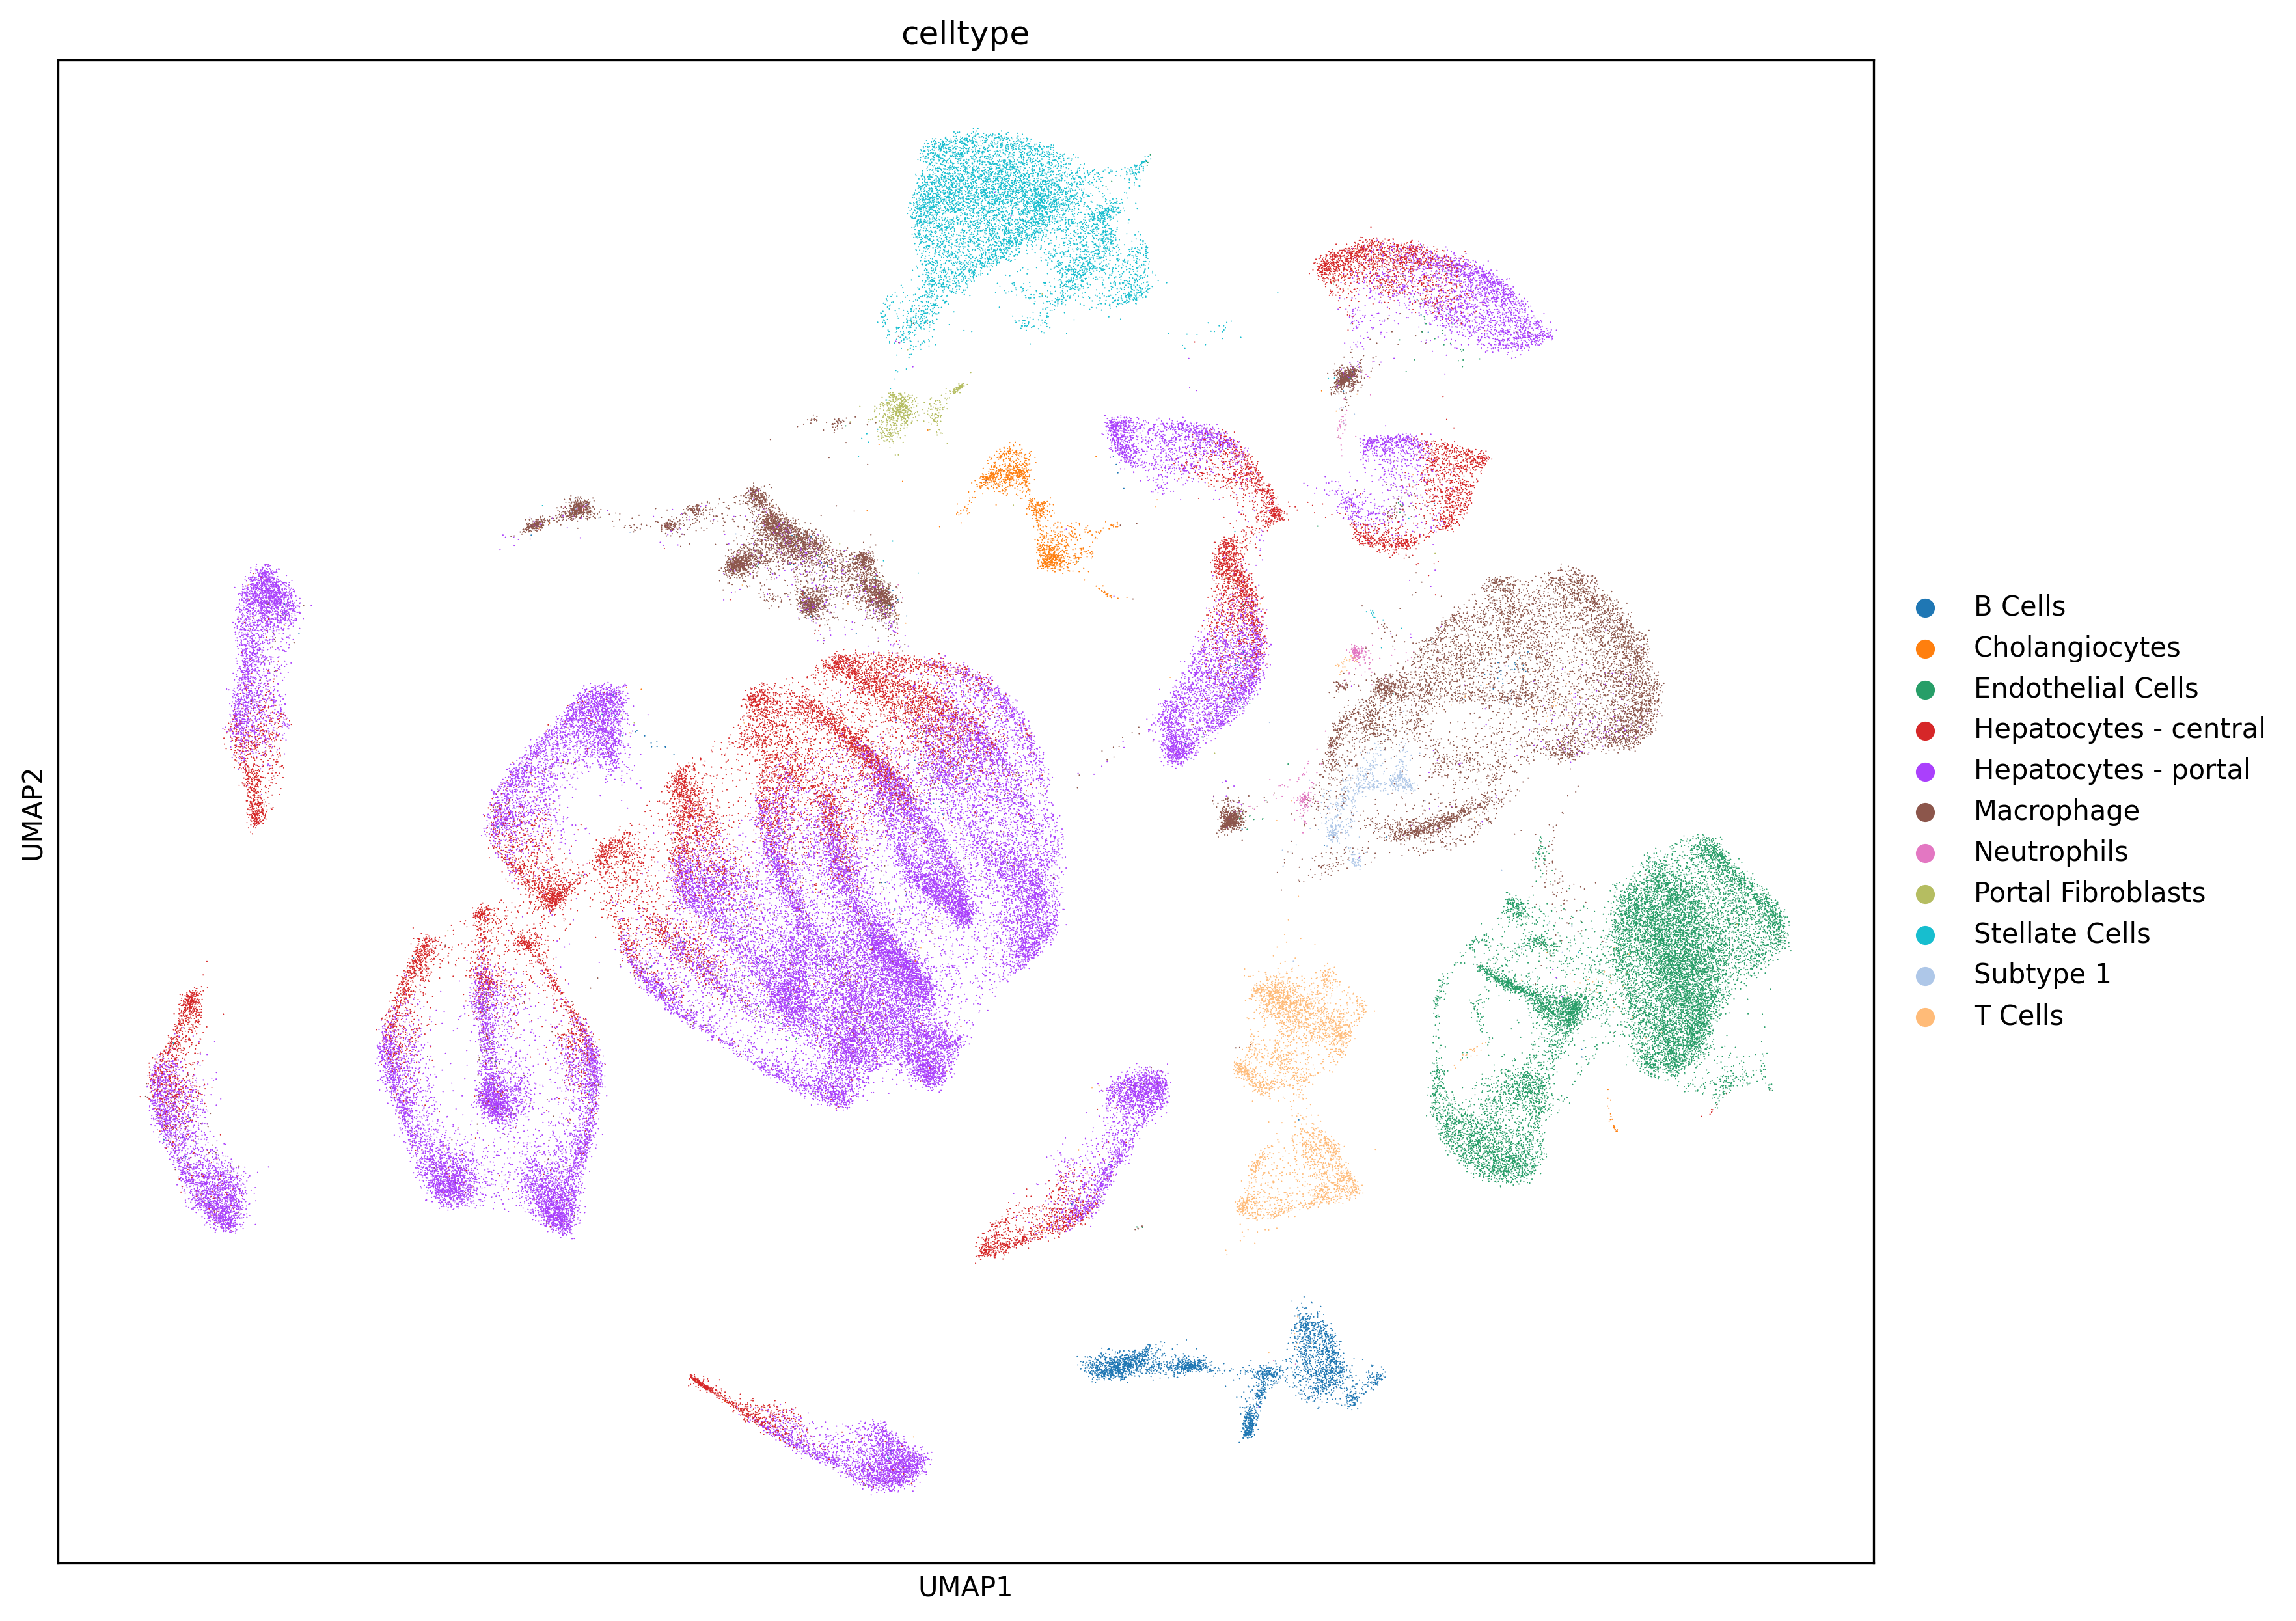
\includegraphics[width=\textwidth]{figures/nault_cell_umap.png}
        \caption{}
        \label{fig:figure1}
    \end{subfigure}%
    \hfill
    \begin{subfigure}[t]{0.49\textwidth}
        \centering
        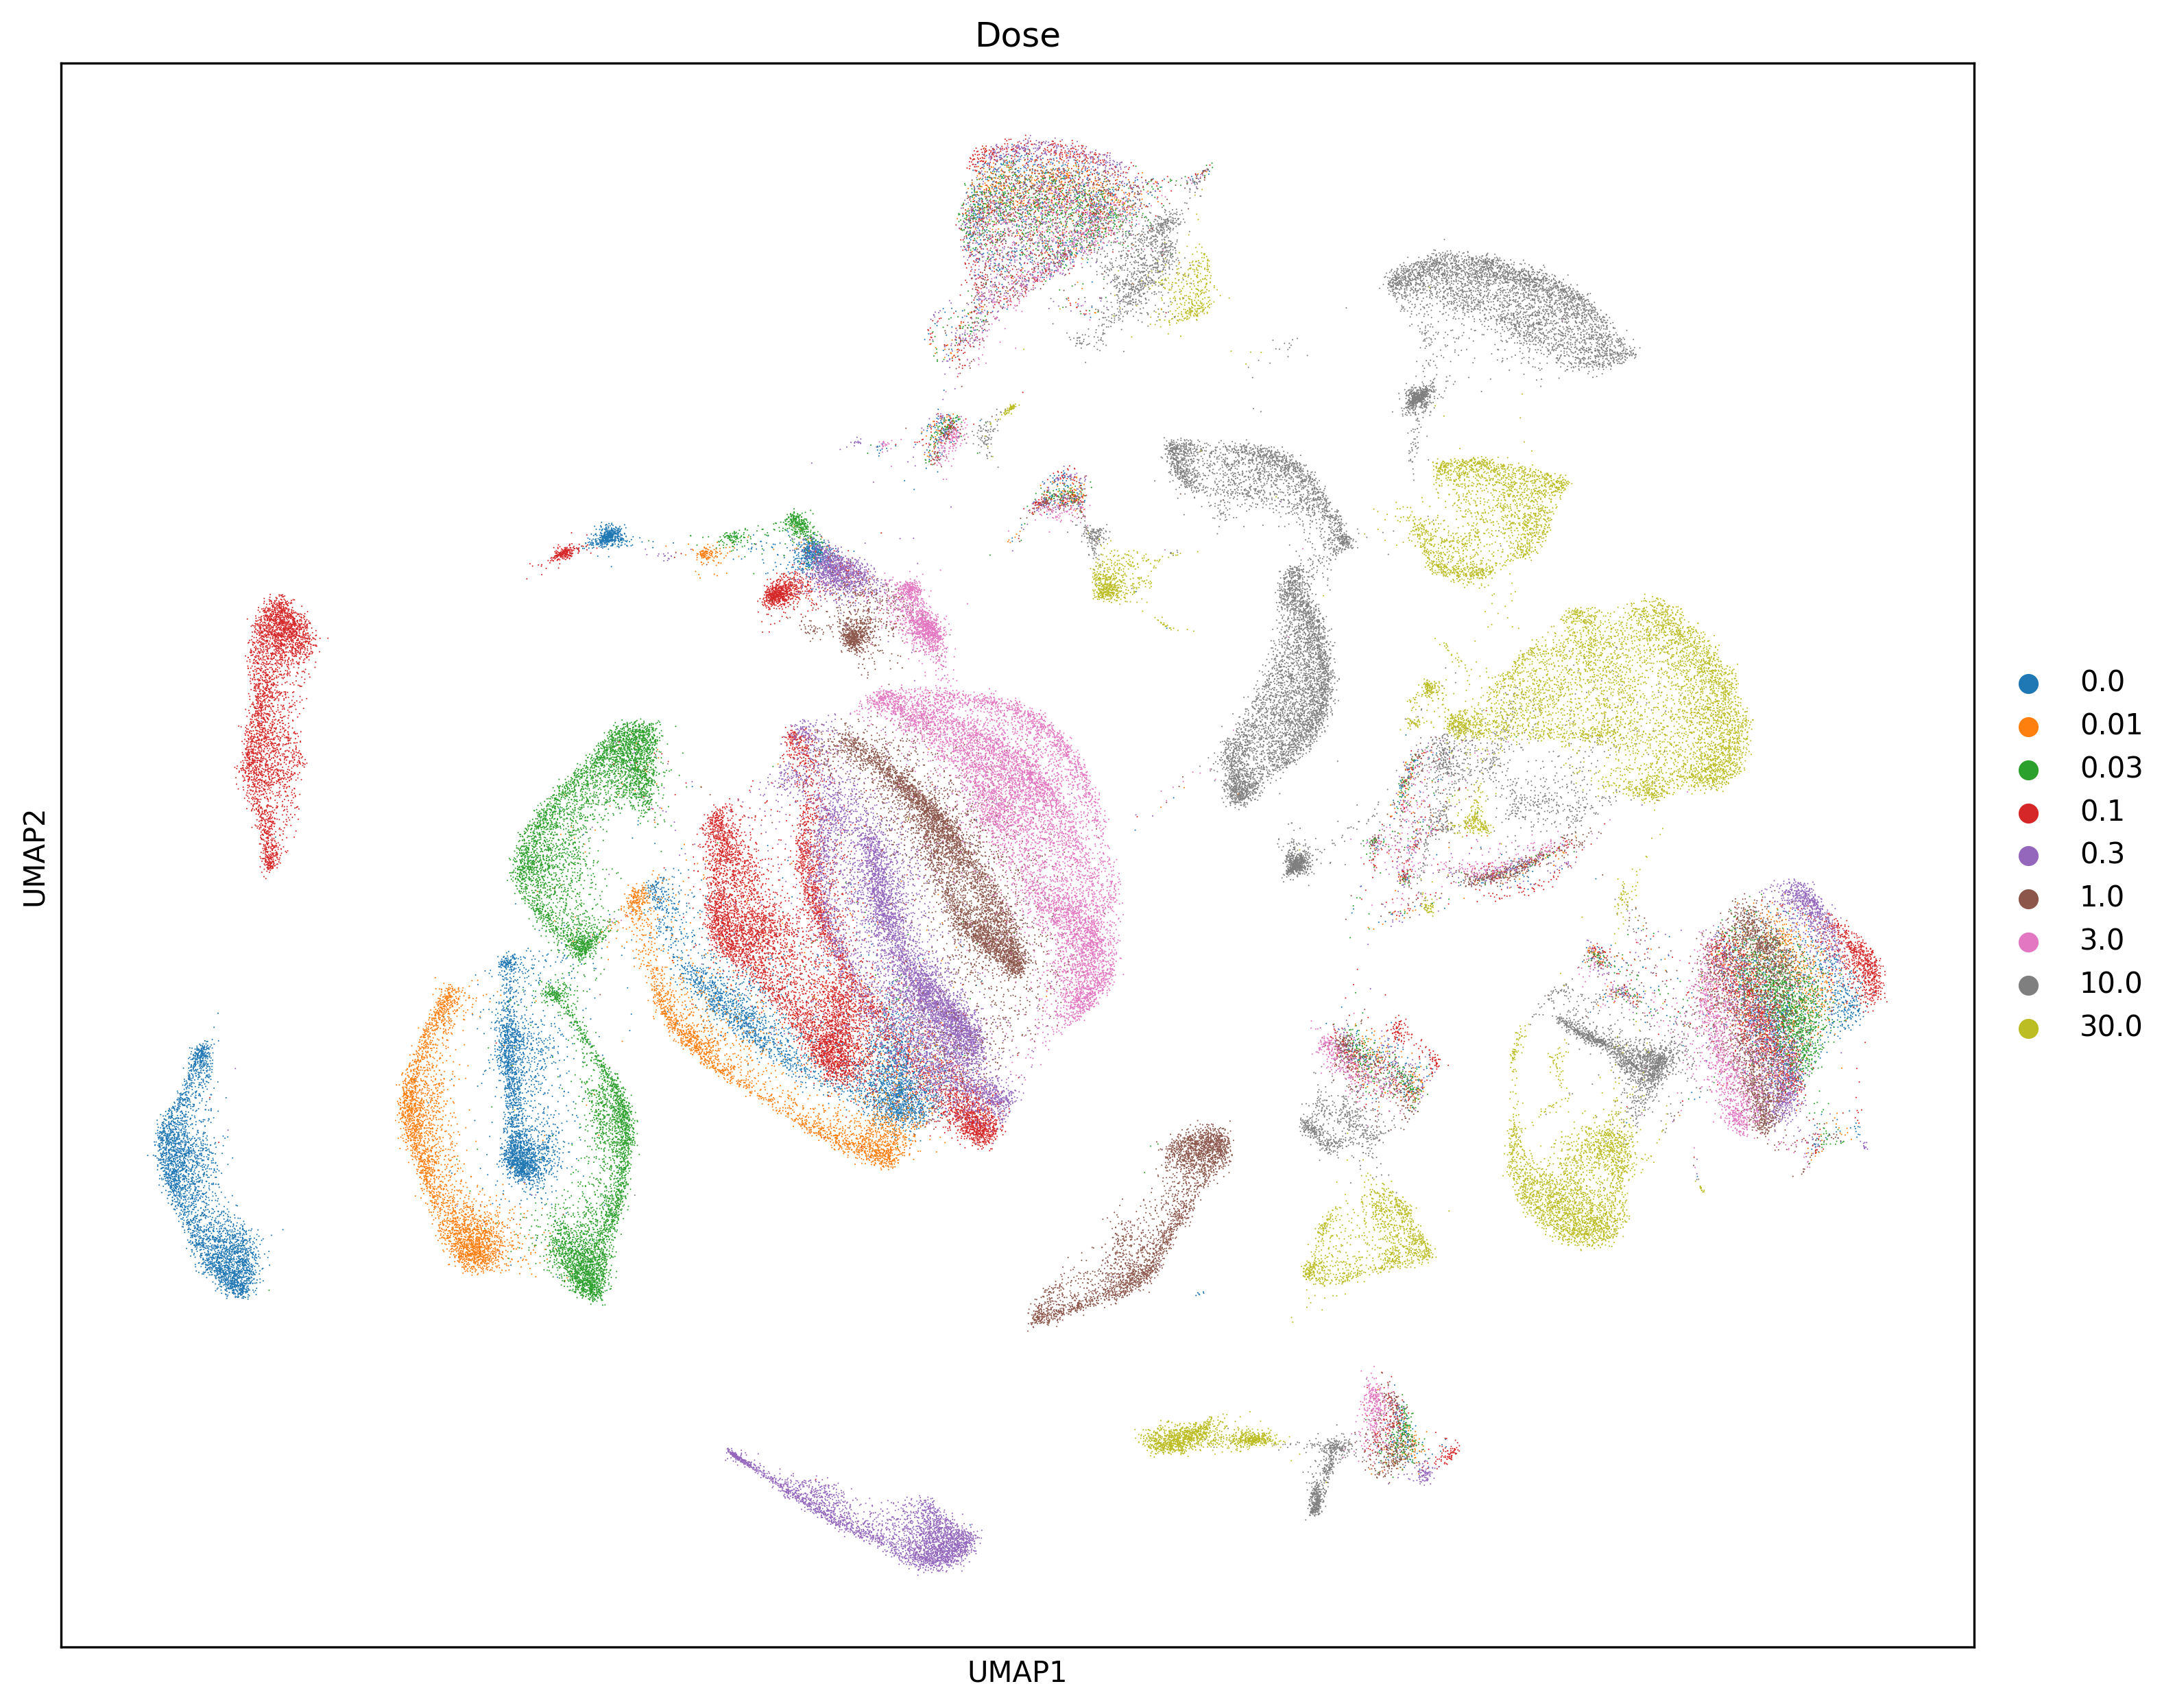
\includegraphics[width=.75\textwidth]{figures/nault_dose_umap.png}
        \caption{}
        \label{fig:figure2}
    \end{subfigure}%
    \hfill
    \begin{subfigure}[b]{\textwidth}
        \centering
        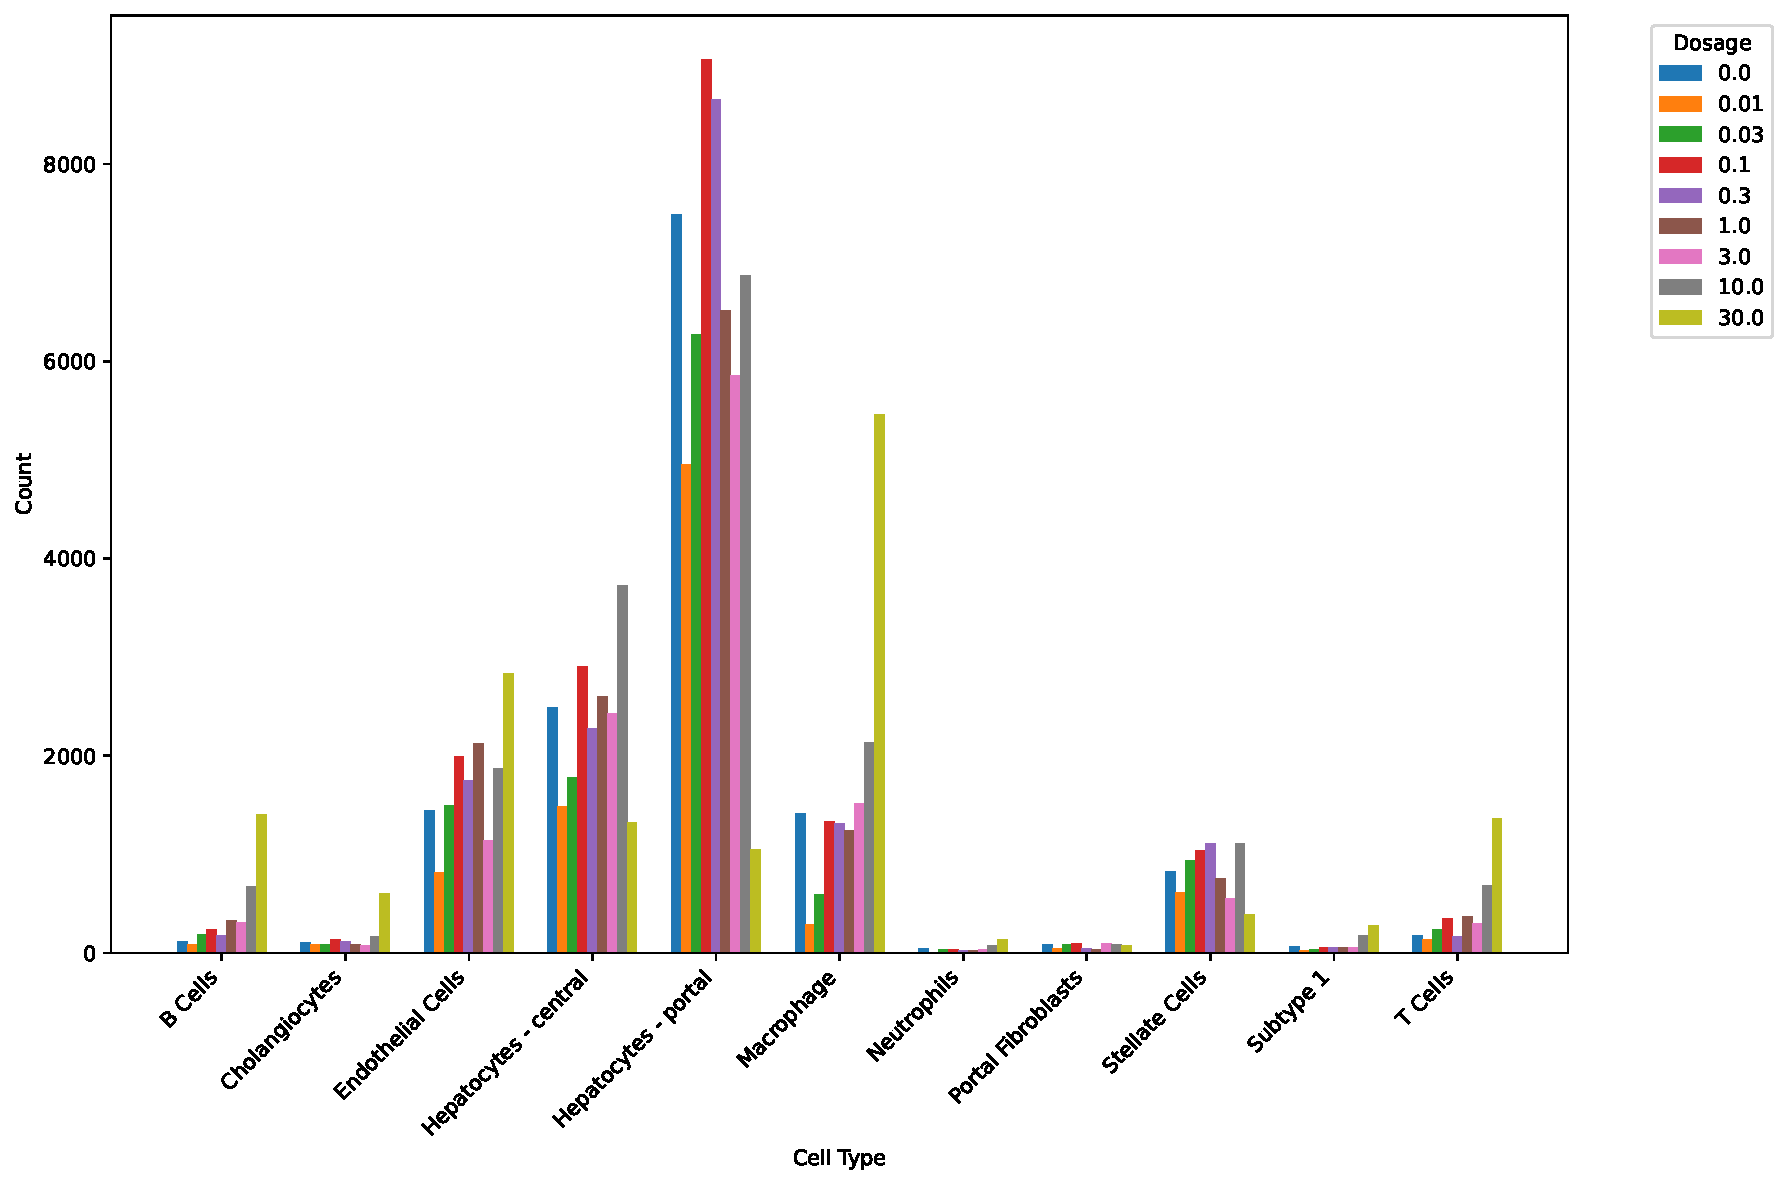
\includegraphics[width=.7\textwidth]{figures/nault_counts.pdf}
        \caption{}
        \label{fig:figure3}
    \end{subfigure}
    \caption{Nault overview}
    \label{fig:combined}
\end{figure}



\begin{figure}
    \centering
    \begin{minipage}{0.4\textwidth}
        \centering
        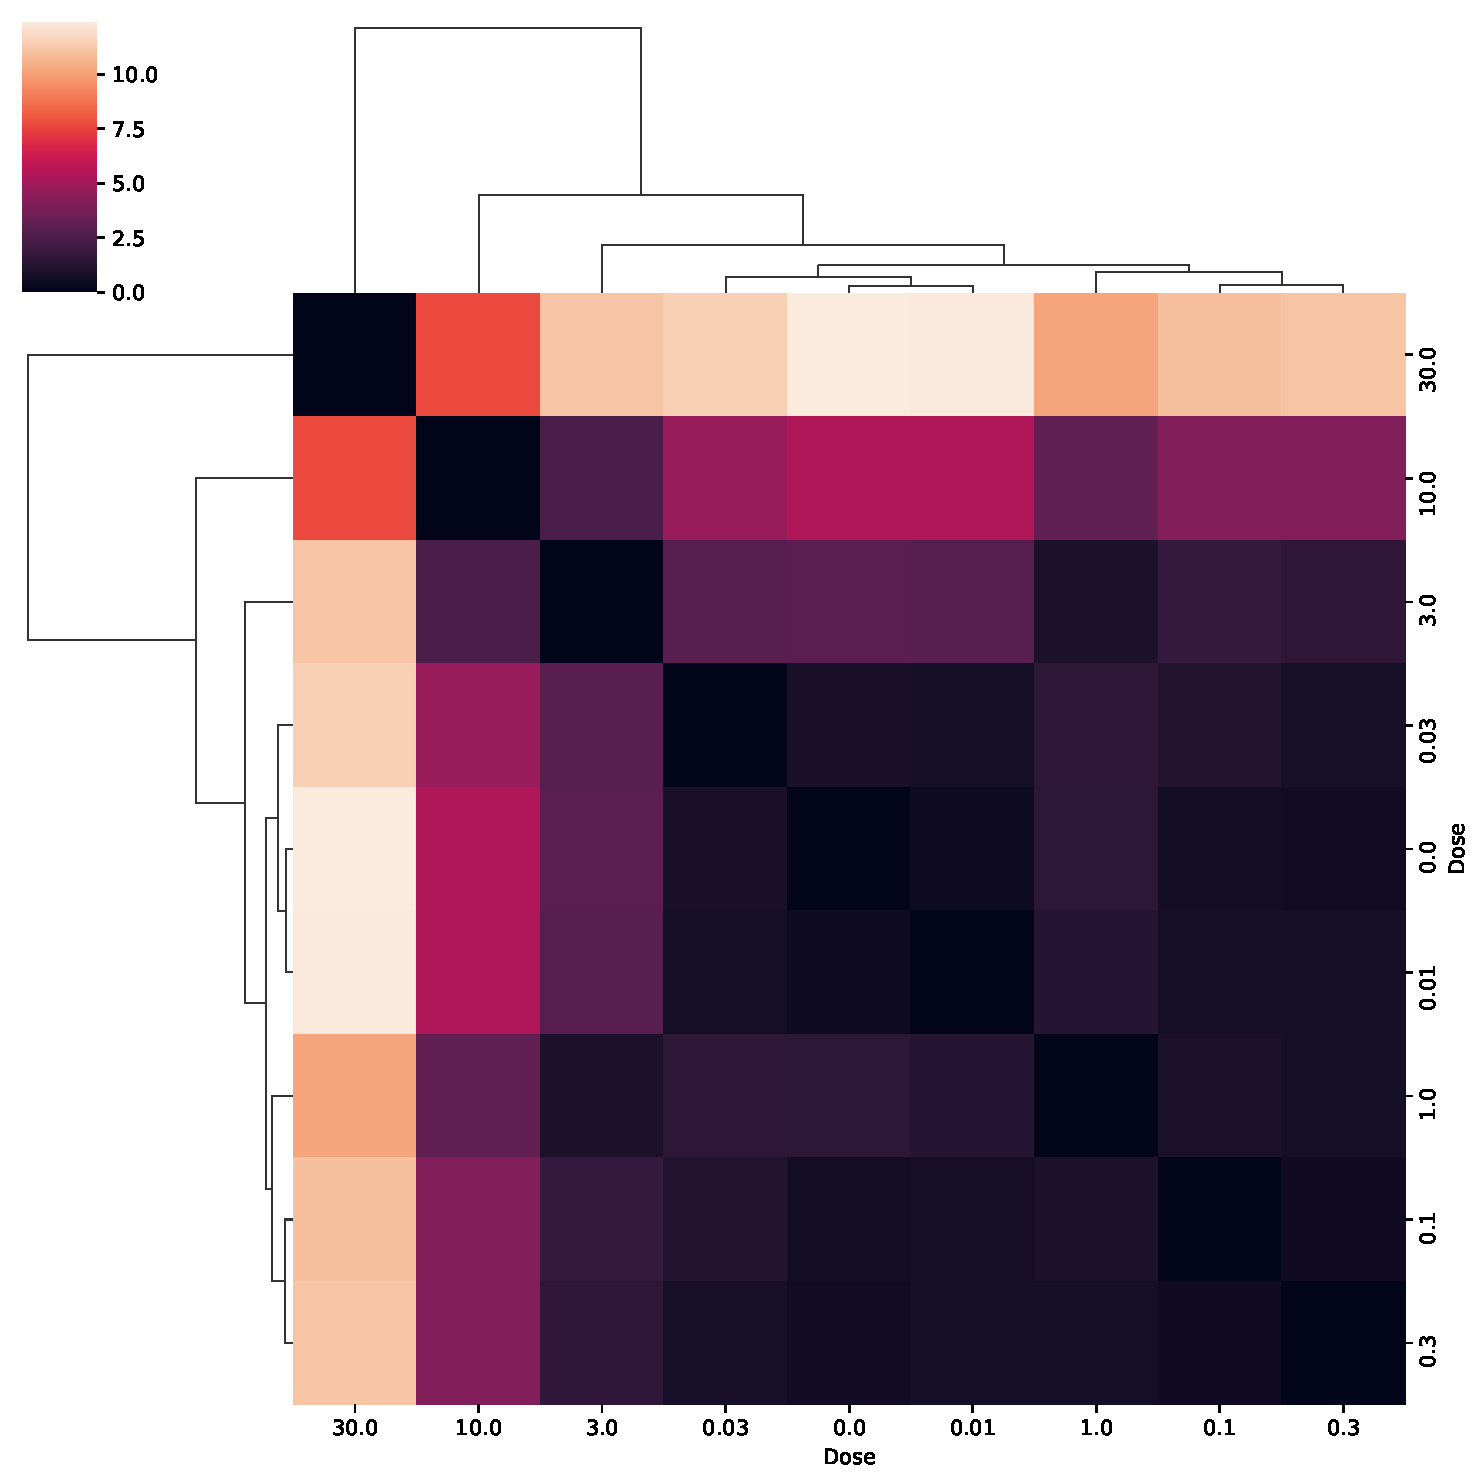
\includegraphics[width=\textwidth]{figures/nault_edistance_clustermap.pdf}
        \caption{E-distance}
    \end{minipage} \hfill
    \begin{minipage}{0.4\textwidth}
        \centering
        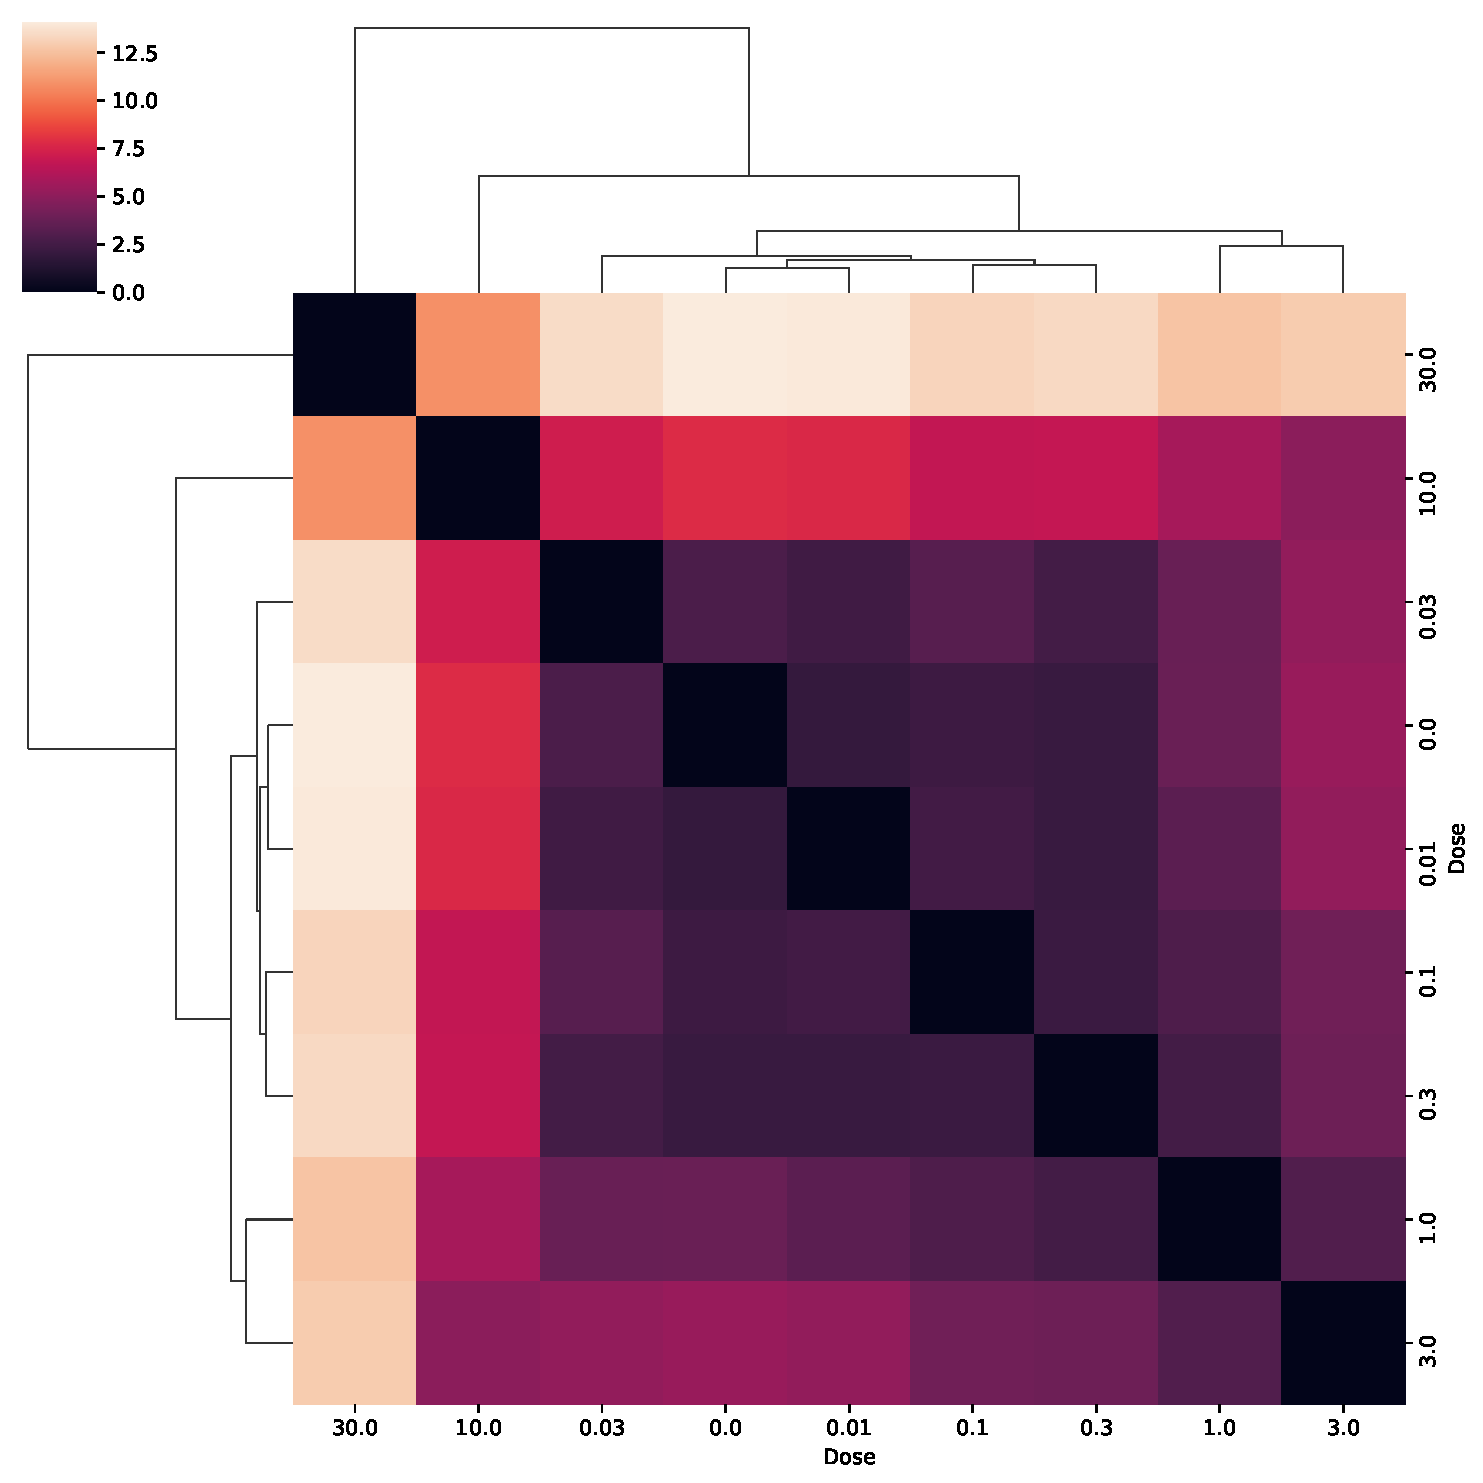
\includegraphics[width=\textwidth]{figures/nault_euclidean_clustermap.pdf}
        \caption{Euclidean}
    \end{minipage}
    \vskip\baselineskip

    \begin{minipage}{0.4\textwidth}
        \centering
        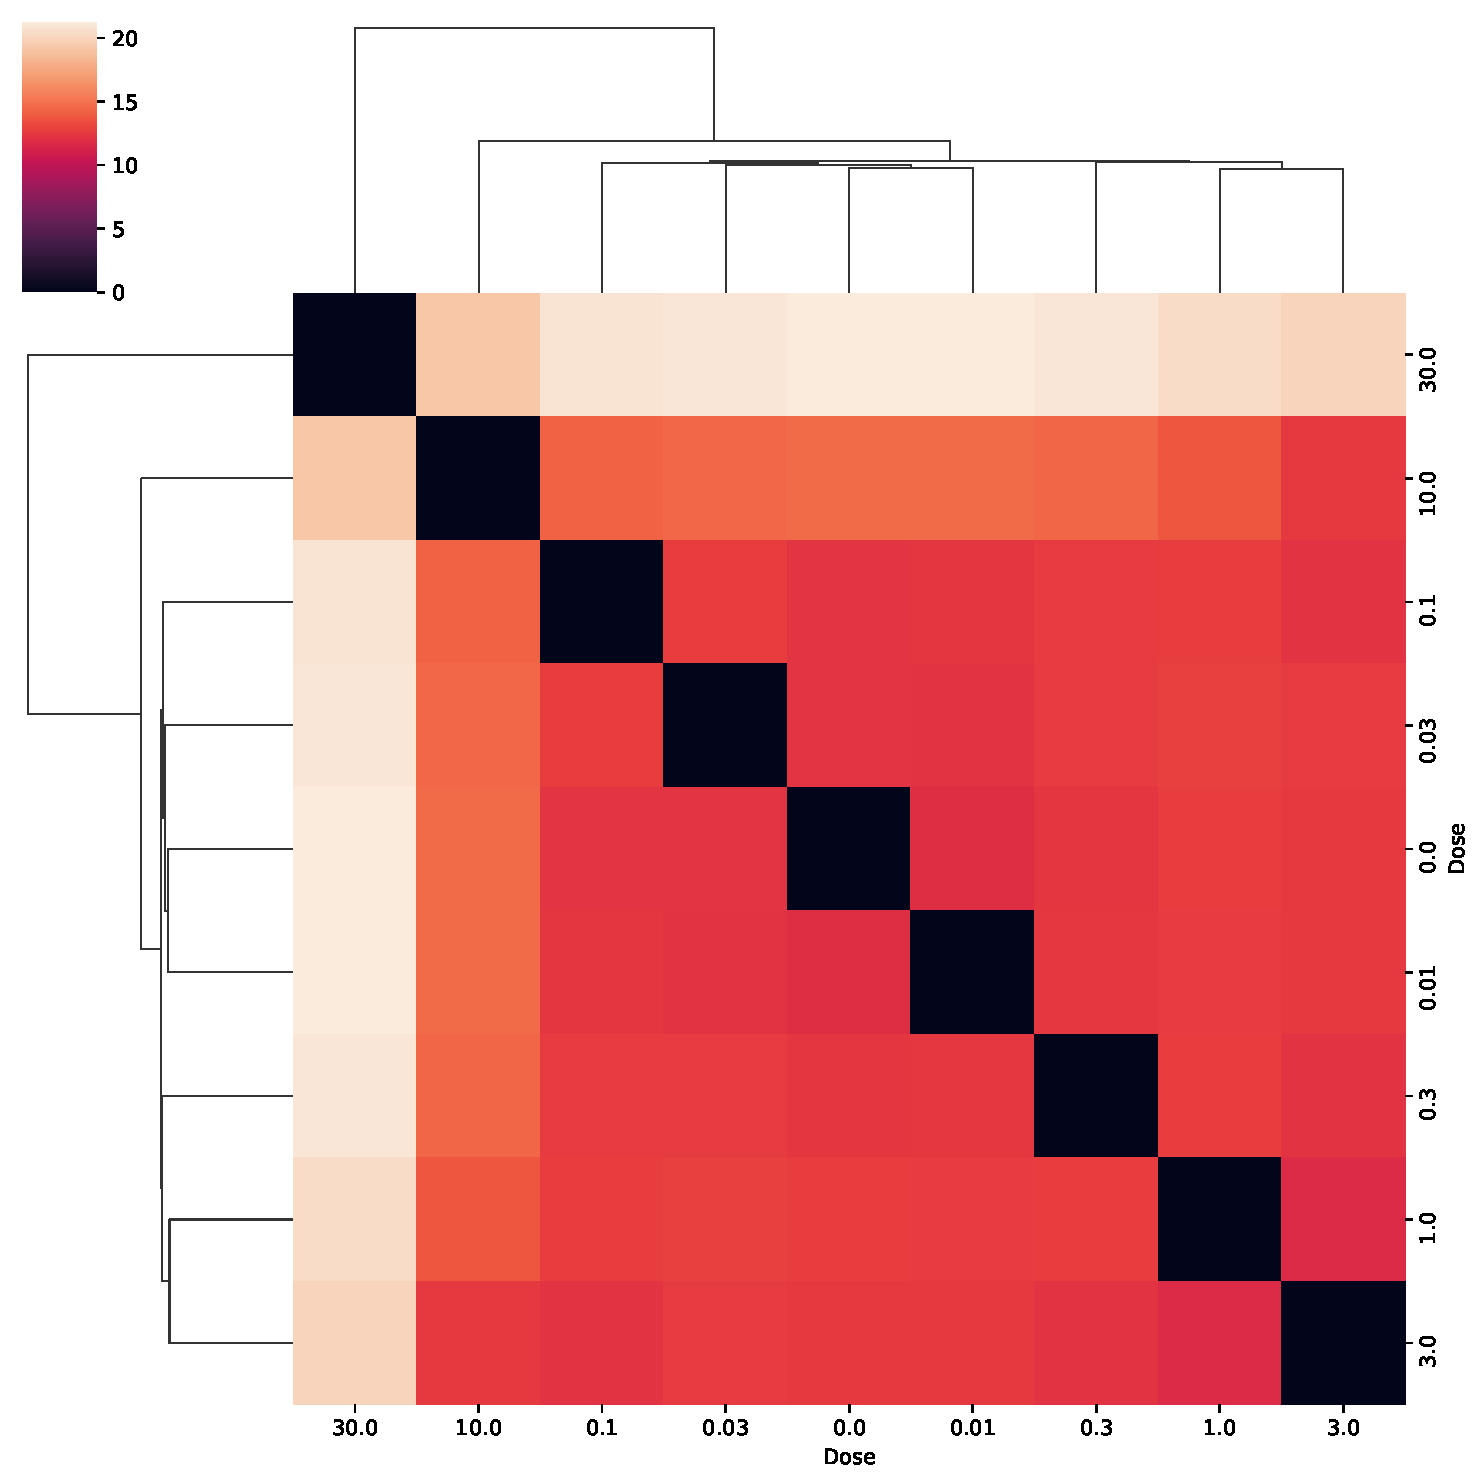
\includegraphics[width=\textwidth]{figures/nault_mean_pairwise_clustermap.pdf}
        \caption{Mean pairwise}
    \end{minipage} \hfill
    \begin{minipage}{0.4\textwidth}
        \centering
        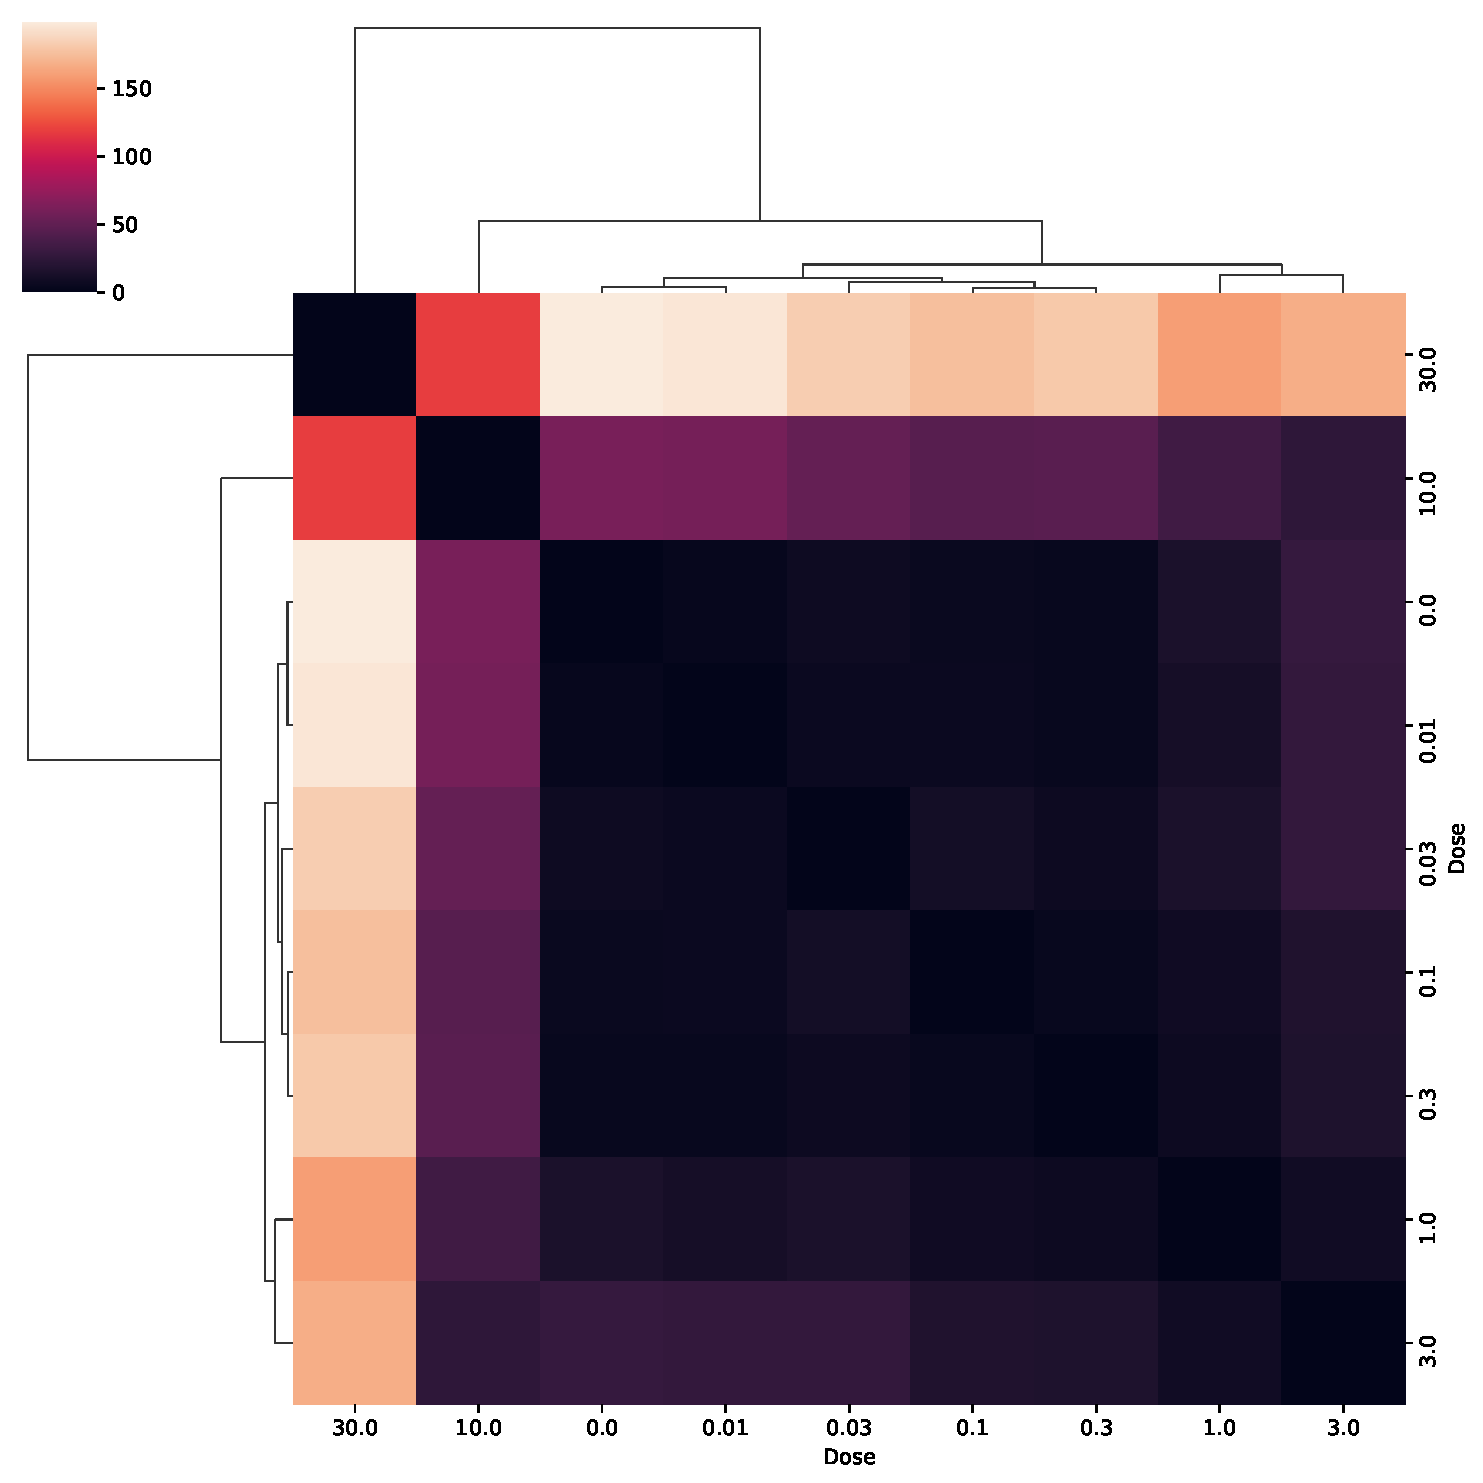
\includegraphics[width=\textwidth]{figures/nault_mmd_clustermap.pdf}
        \caption{MMD}
    \end{minipage}
    \vskip\baselineskip

    \begin{minipage}{0.4\textwidth}
        \centering
        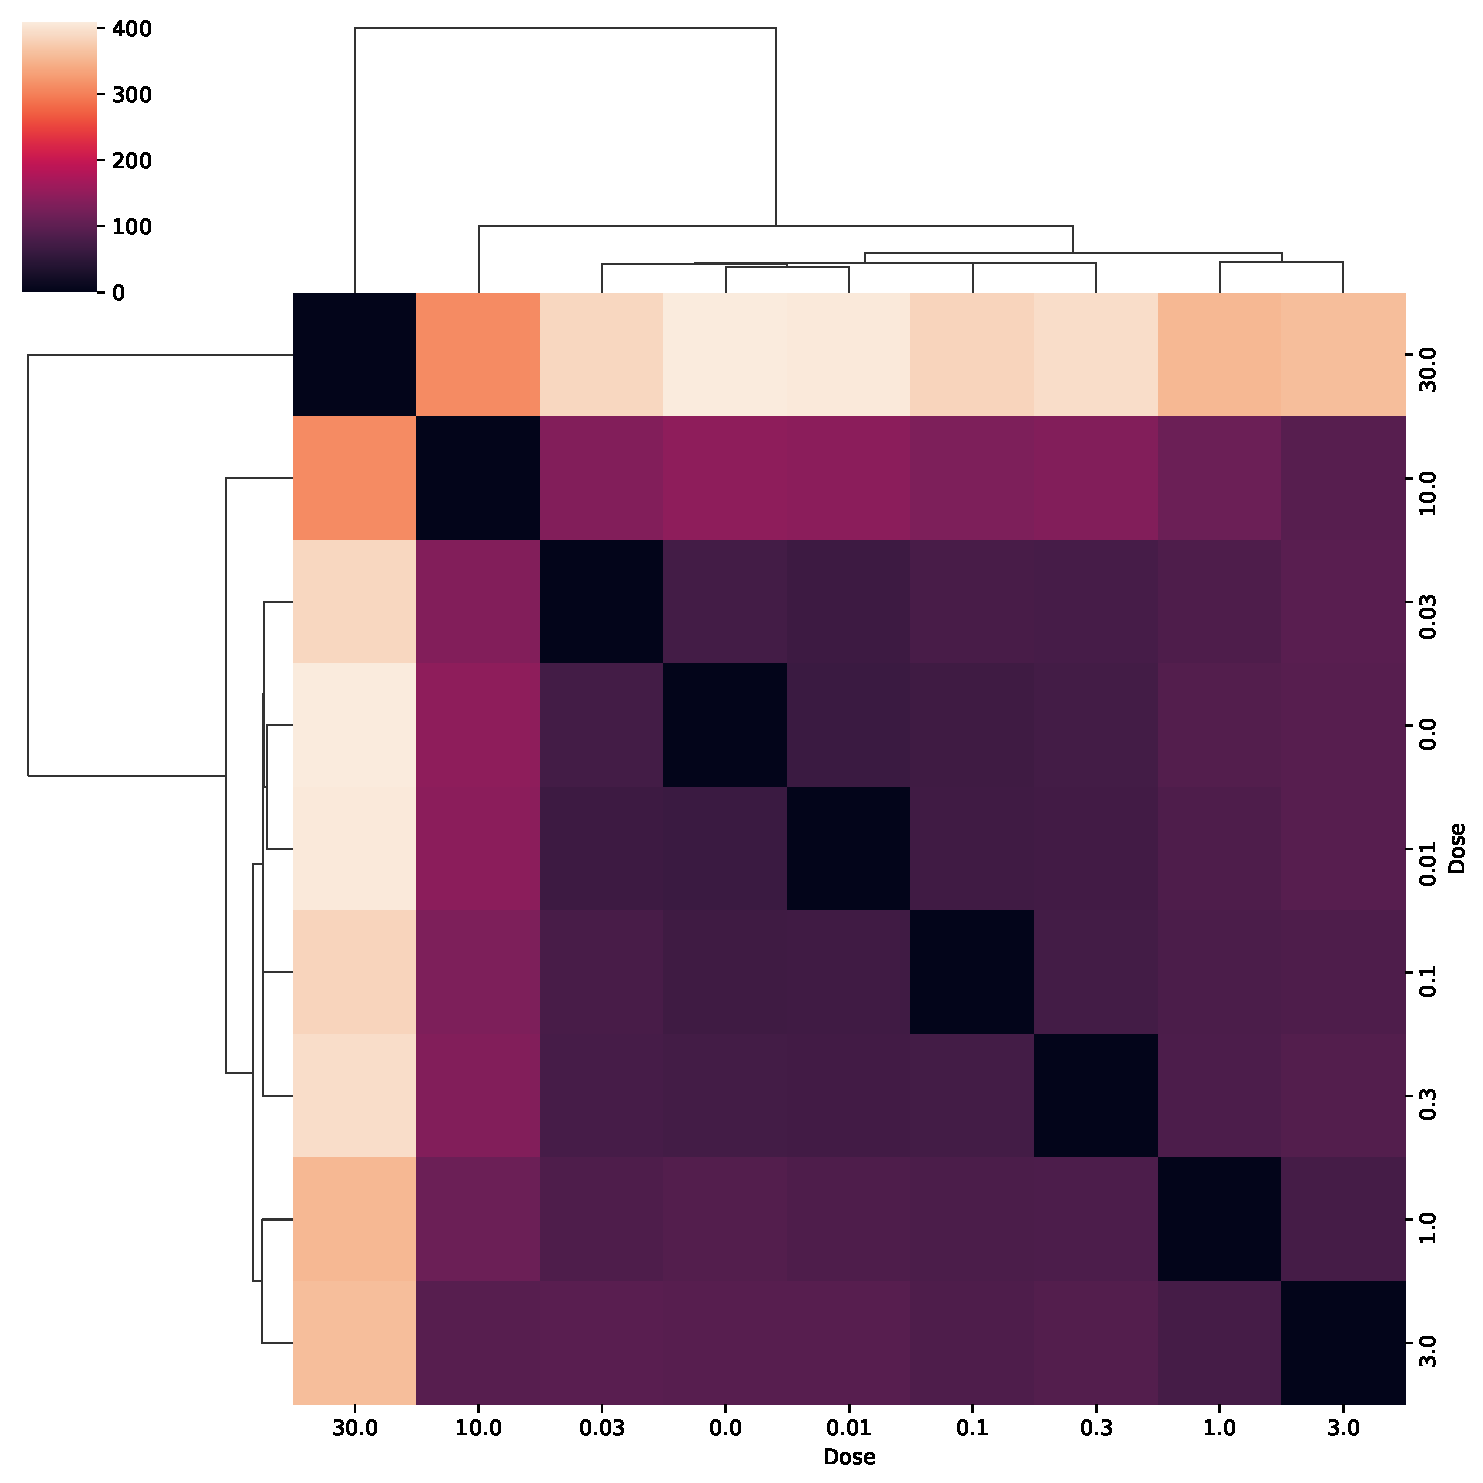
\includegraphics[width=\textwidth]{figures/nault_wasserstein_clustermap.pdf}
        \caption{Wasserstein}
    \end{minipage}
    \caption{Distance metrics across all cell types per dosage}
\end{figure}

\begin{figure}
    \centering
    \begin{minipage}{0.4\textwidth}
        \centering
        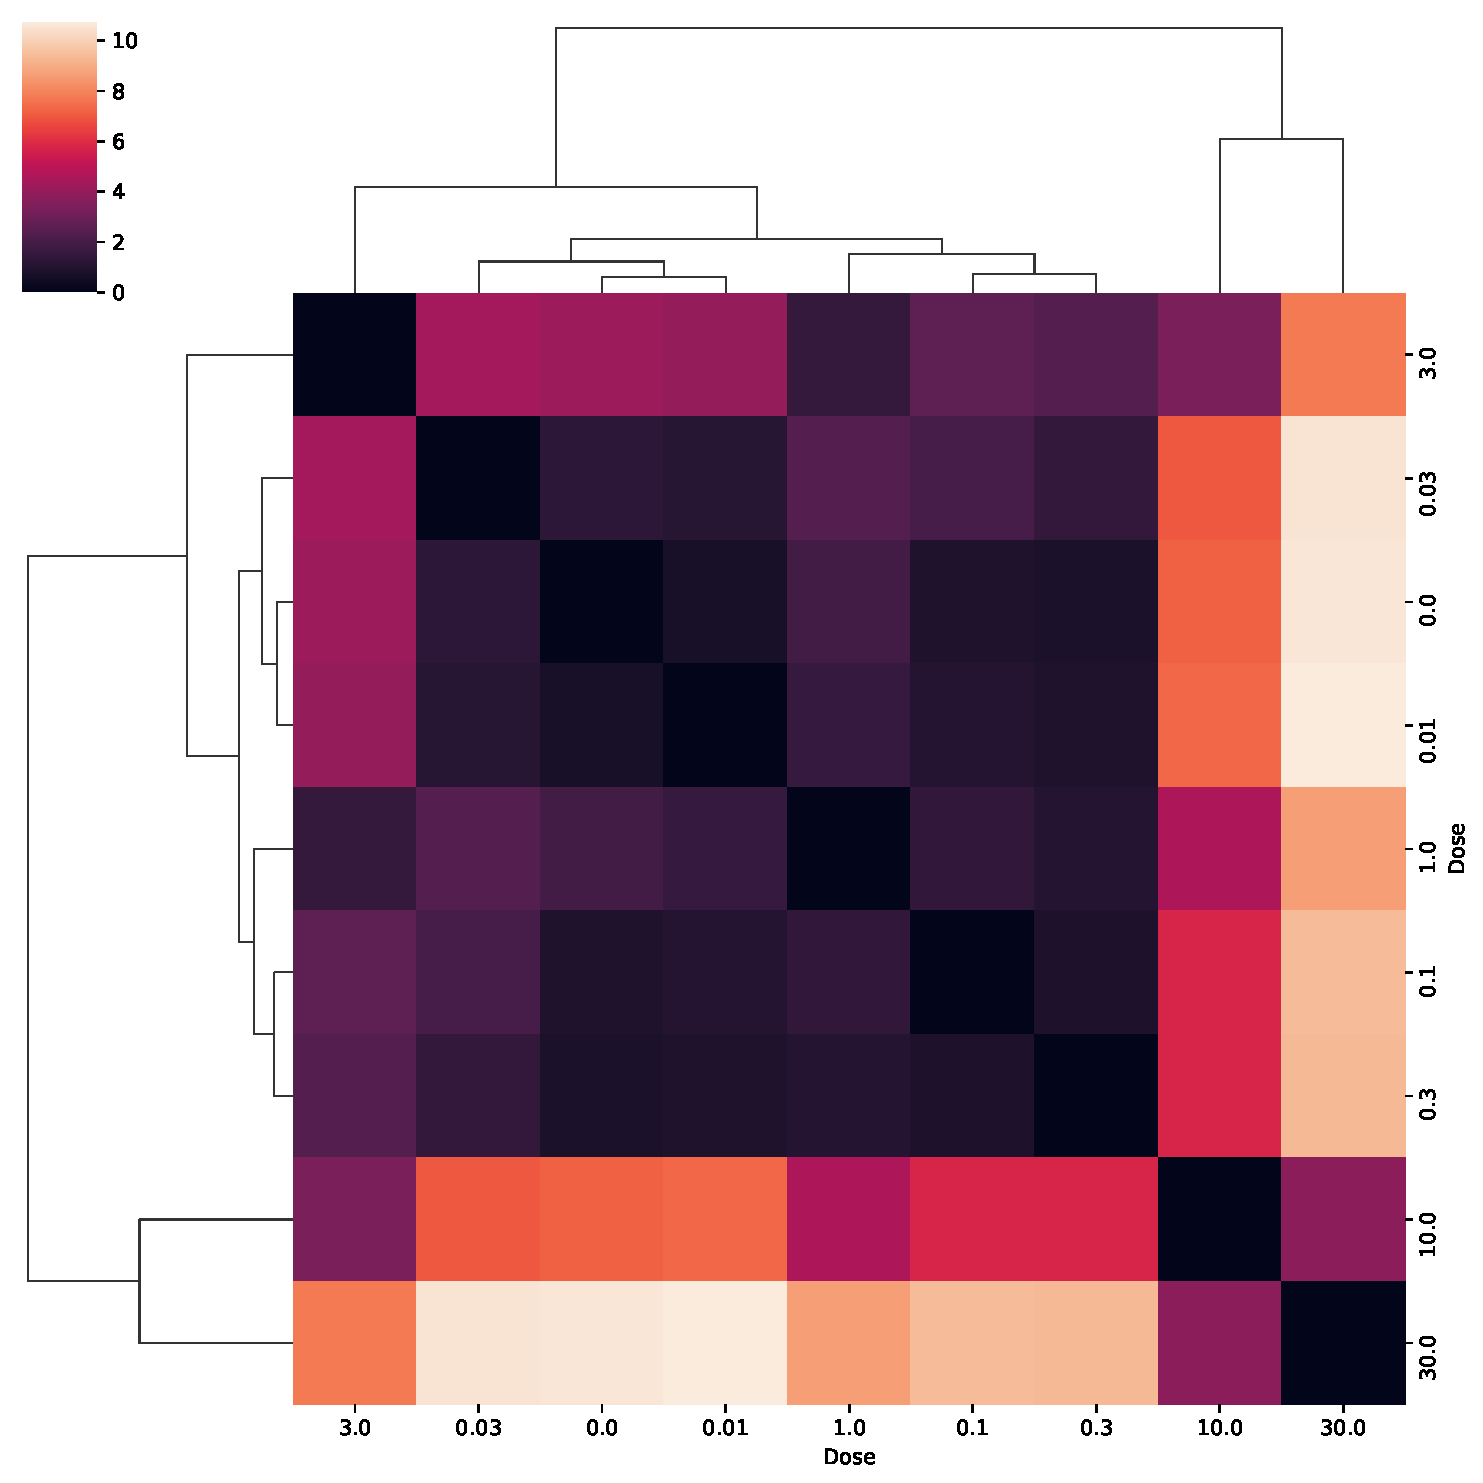
\includegraphics[width=\textwidth]{figures/hepatocytes_edistance_clustermap.pdf}
        \caption{E-distance}
    \end{minipage} \hfill
    \begin{minipage}{0.4\textwidth}
        \centering
        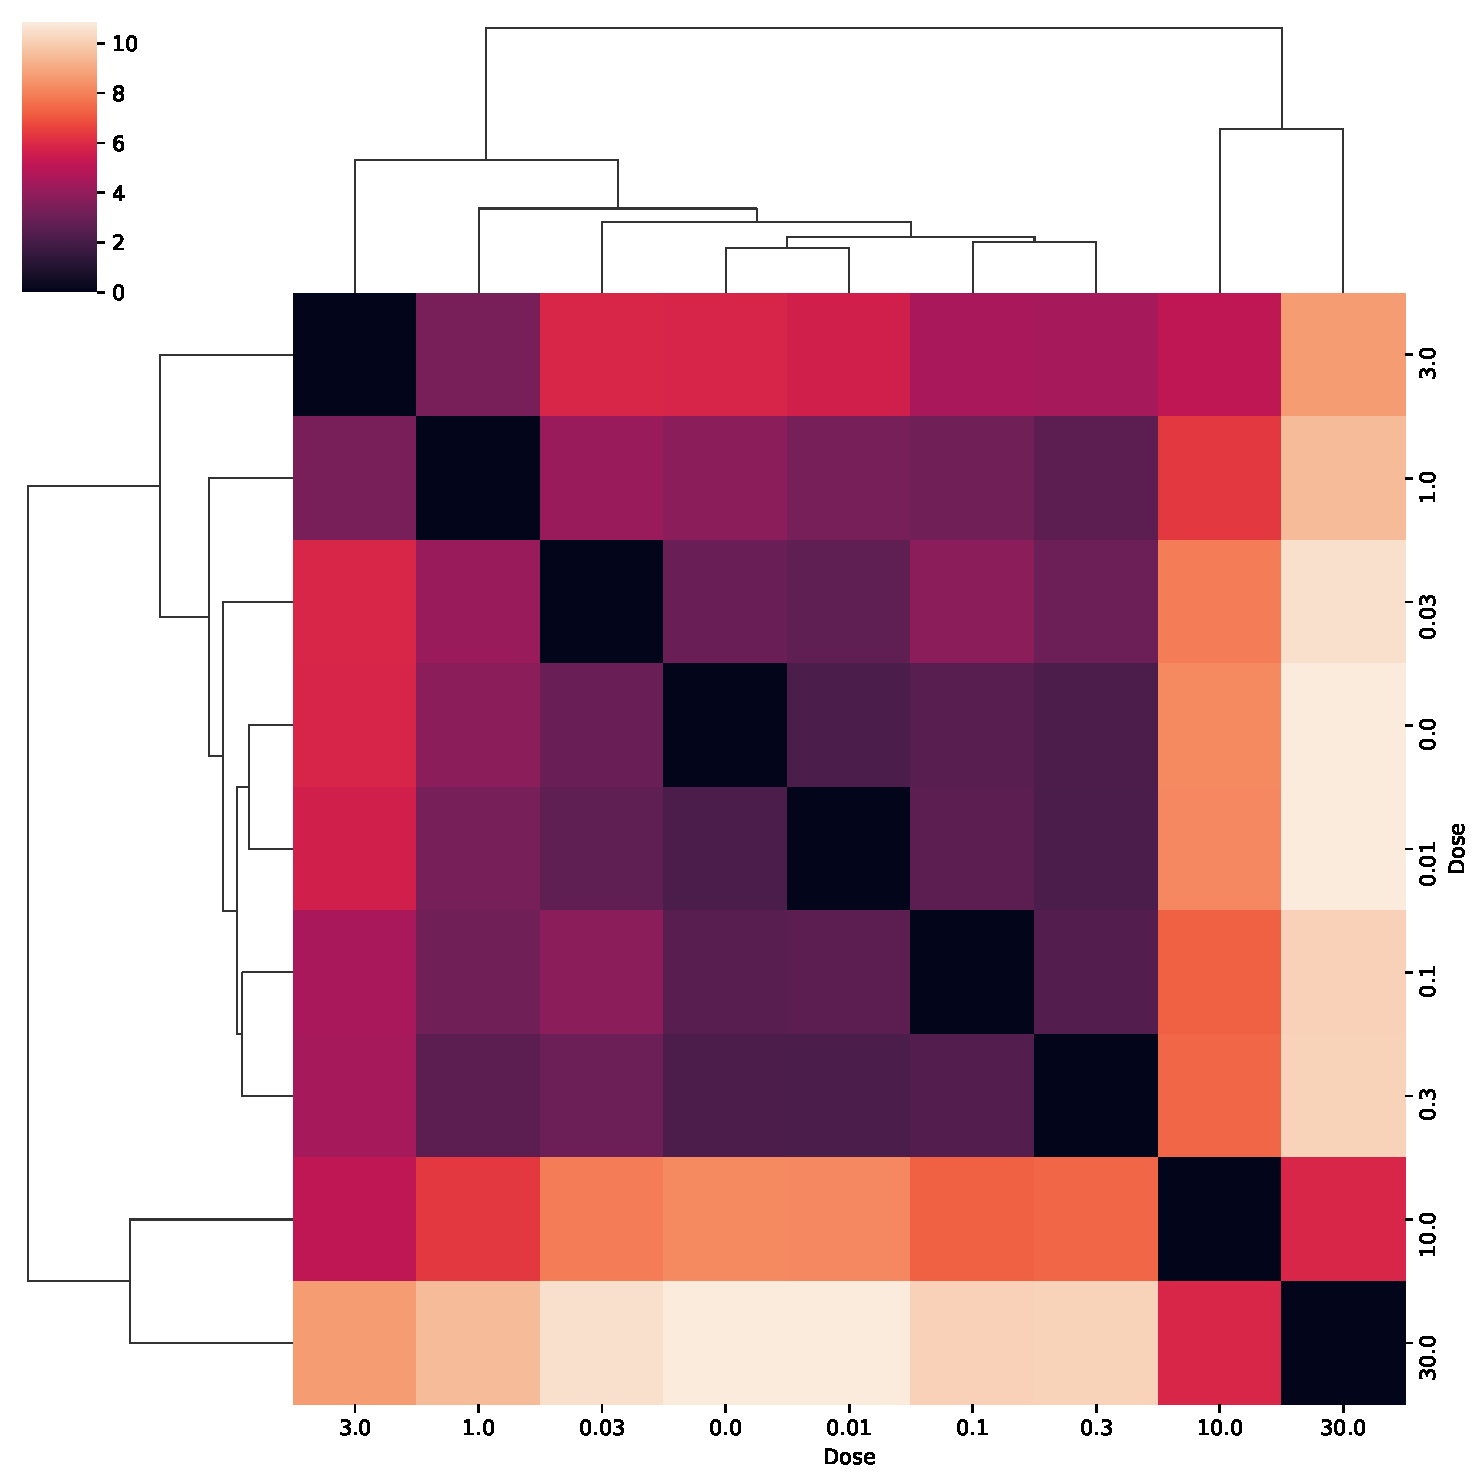
\includegraphics[width=\textwidth]{figures/hepatocytes_euclidean_clustermap.pdf}
        \caption{Euclidean}
    \end{minipage}
    \vskip\baselineskip

    \begin{minipage}{0.4\textwidth}
        \centering
        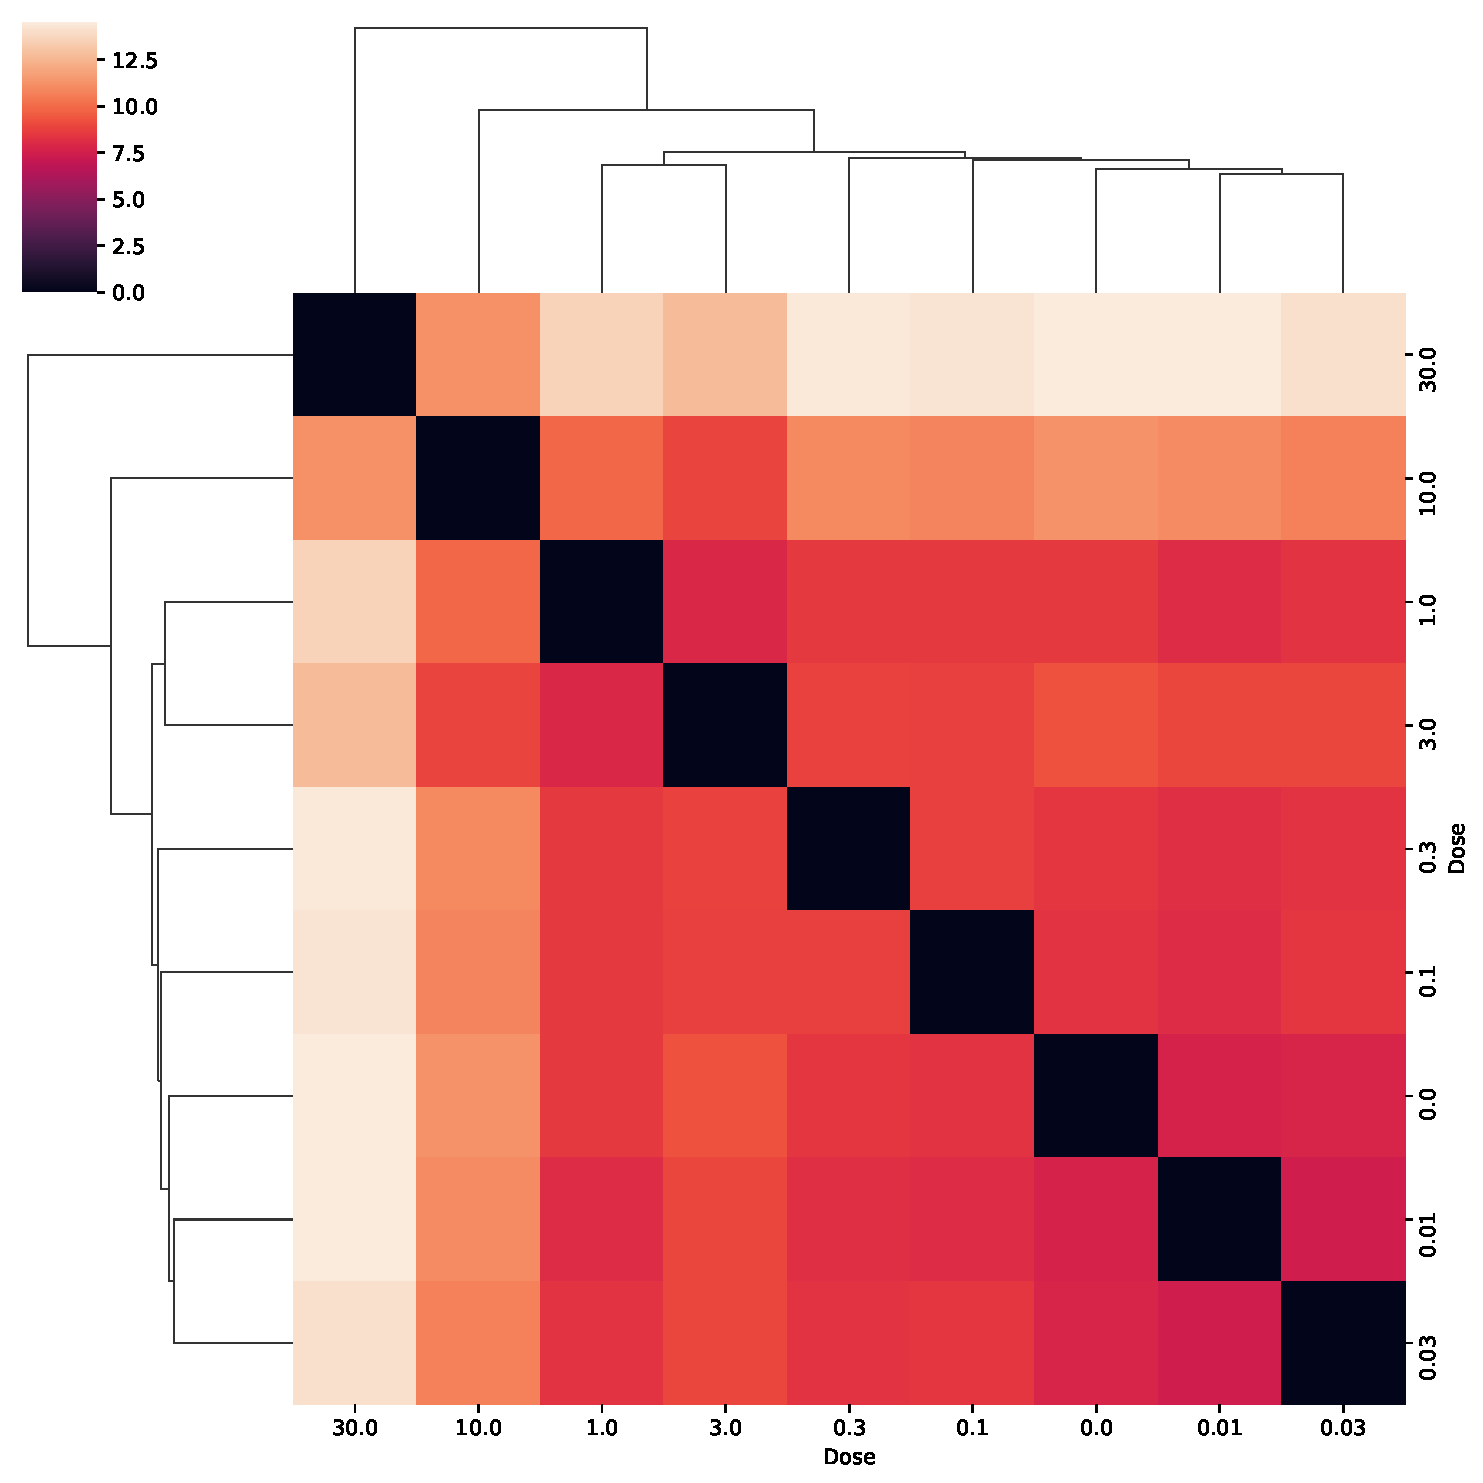
\includegraphics[width=\textwidth]{figures/hepatocytes_mean_pairwise_clustermap.pdf}
        \caption{Mean pairwise}
    \end{minipage} \hfill
    \begin{minipage}{0.4\textwidth}
        \centering
        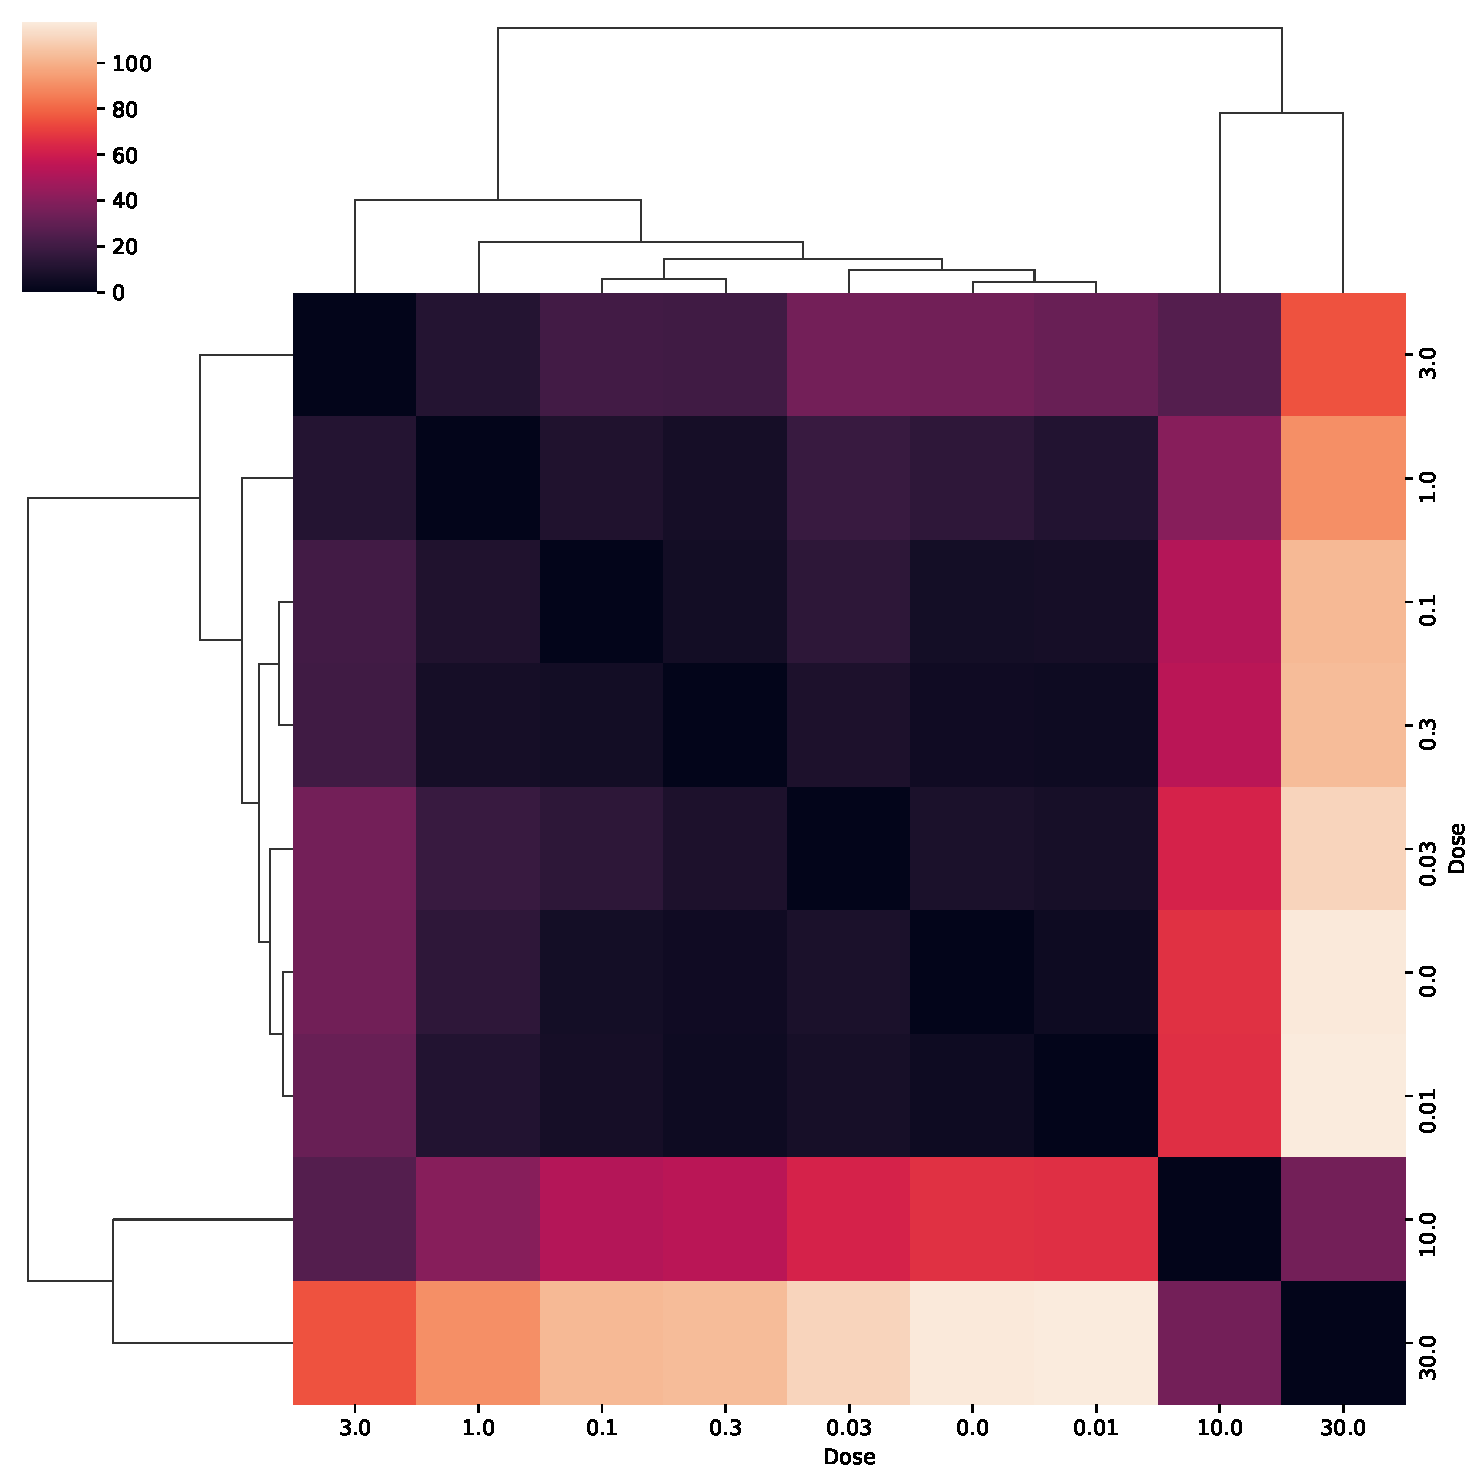
\includegraphics[width=\textwidth]{figures/hepatocytes_mmd_clustermap.pdf}
        \caption{MMD}
    \end{minipage}
    \vskip\baselineskip

    \begin{minipage}{0.4\textwidth}
        \centering
        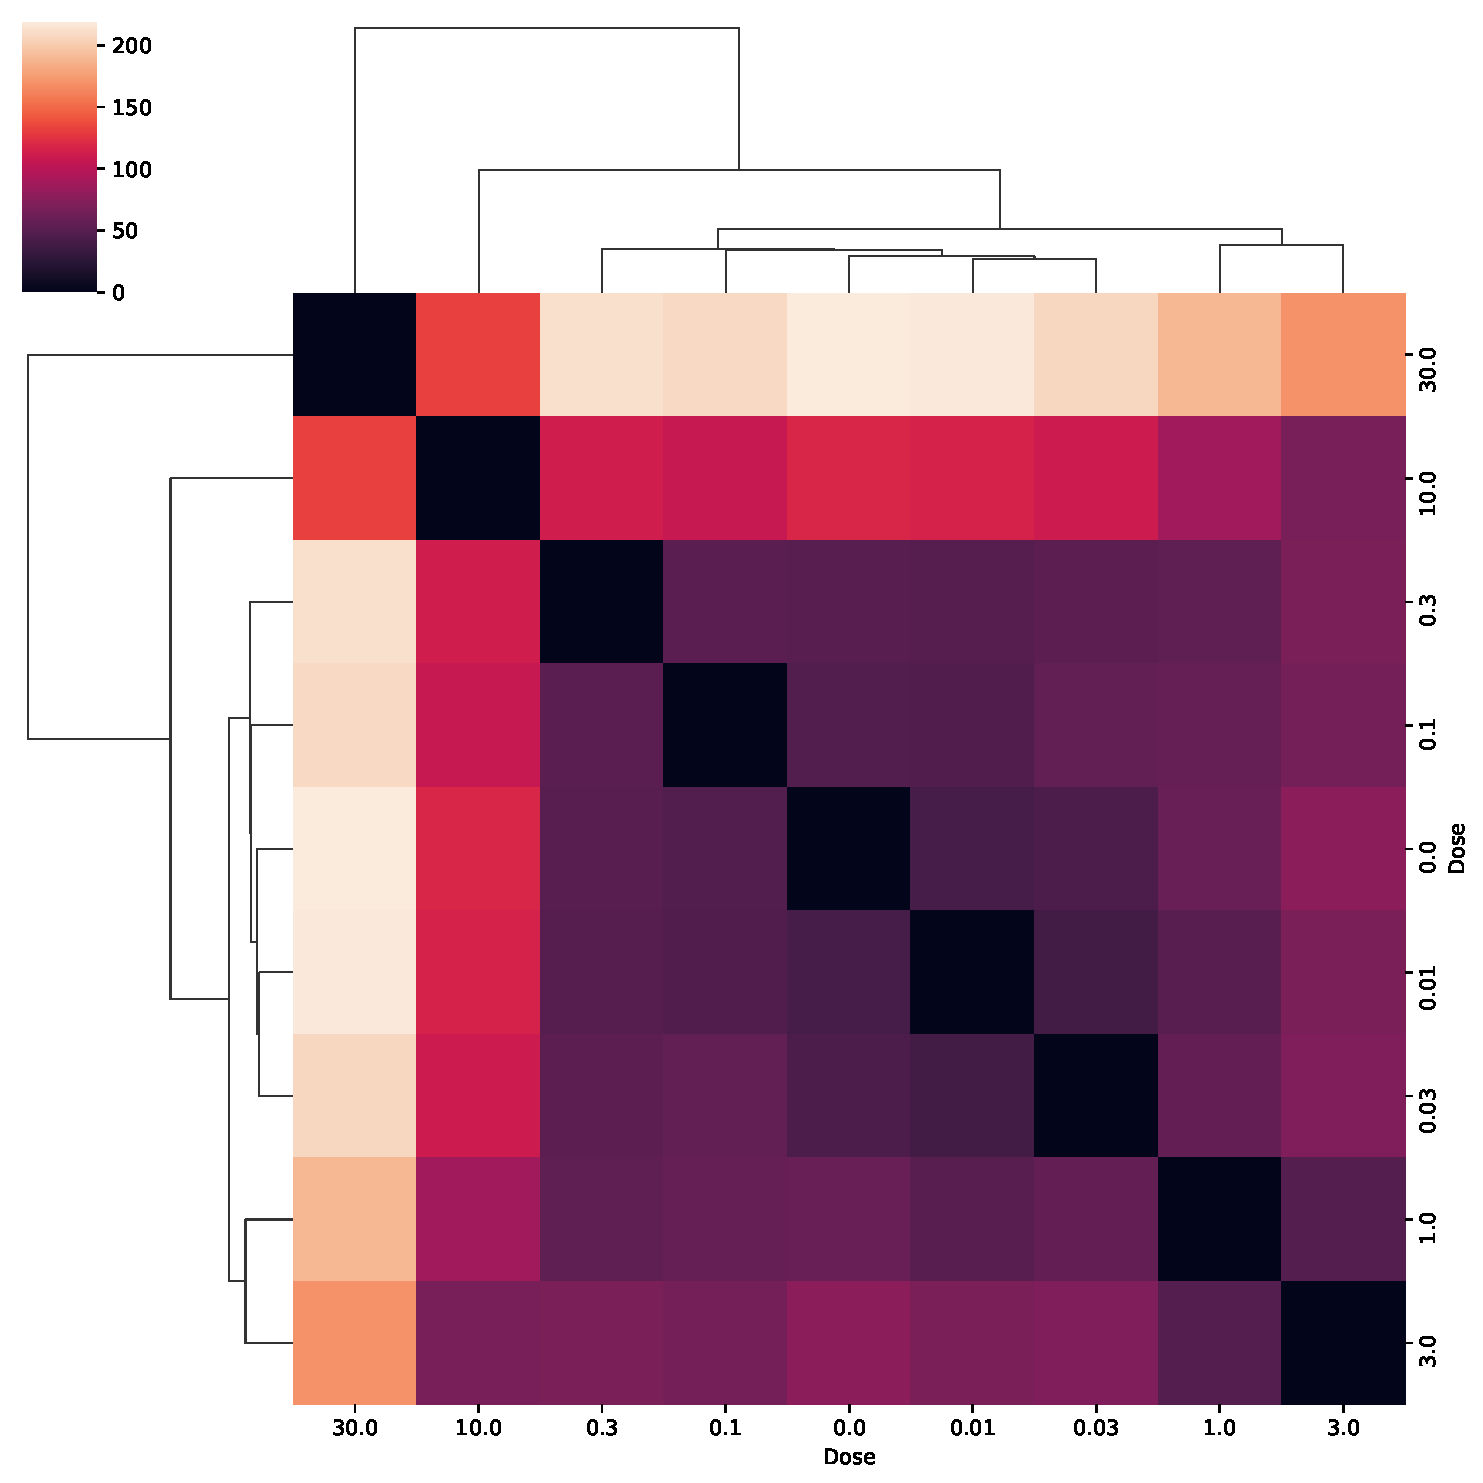
\includegraphics[width=\textwidth]{figures/hepatocytes_wasserstein_clustermap.pdf}
        \caption{Wasserstein}
    \end{minipage}
    \caption{Distance metrics for cell type Hepatocytes - portal per dosage}
\end{figure}

\begin{figure}
    \centering
    \begin{minipage}{0.4\textwidth}
        \centering
        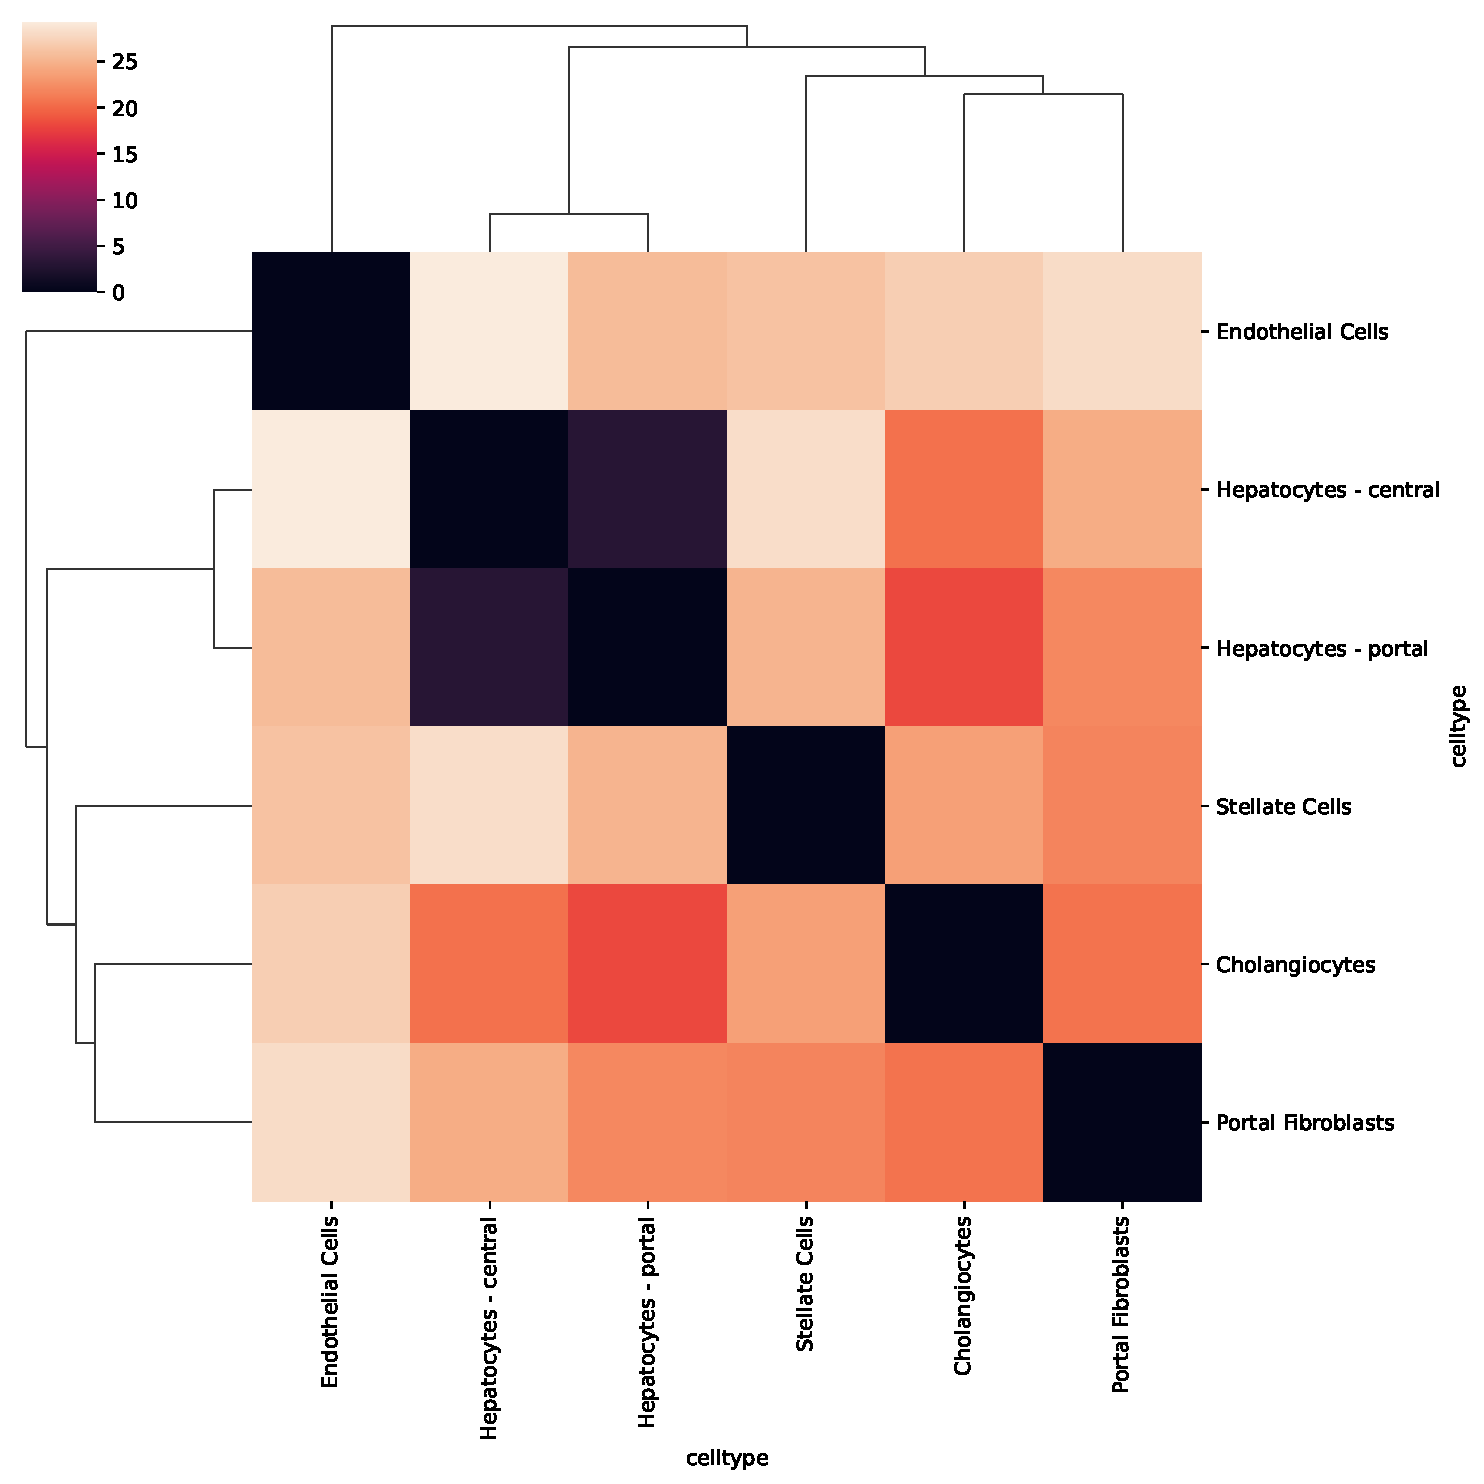
\includegraphics[width=\textwidth]{figures/dose_highest_edistance_clustermap.pdf}
        \caption{E-distance}
    \end{minipage} \hfill
    \begin{minipage}{0.4\textwidth}
        \centering
        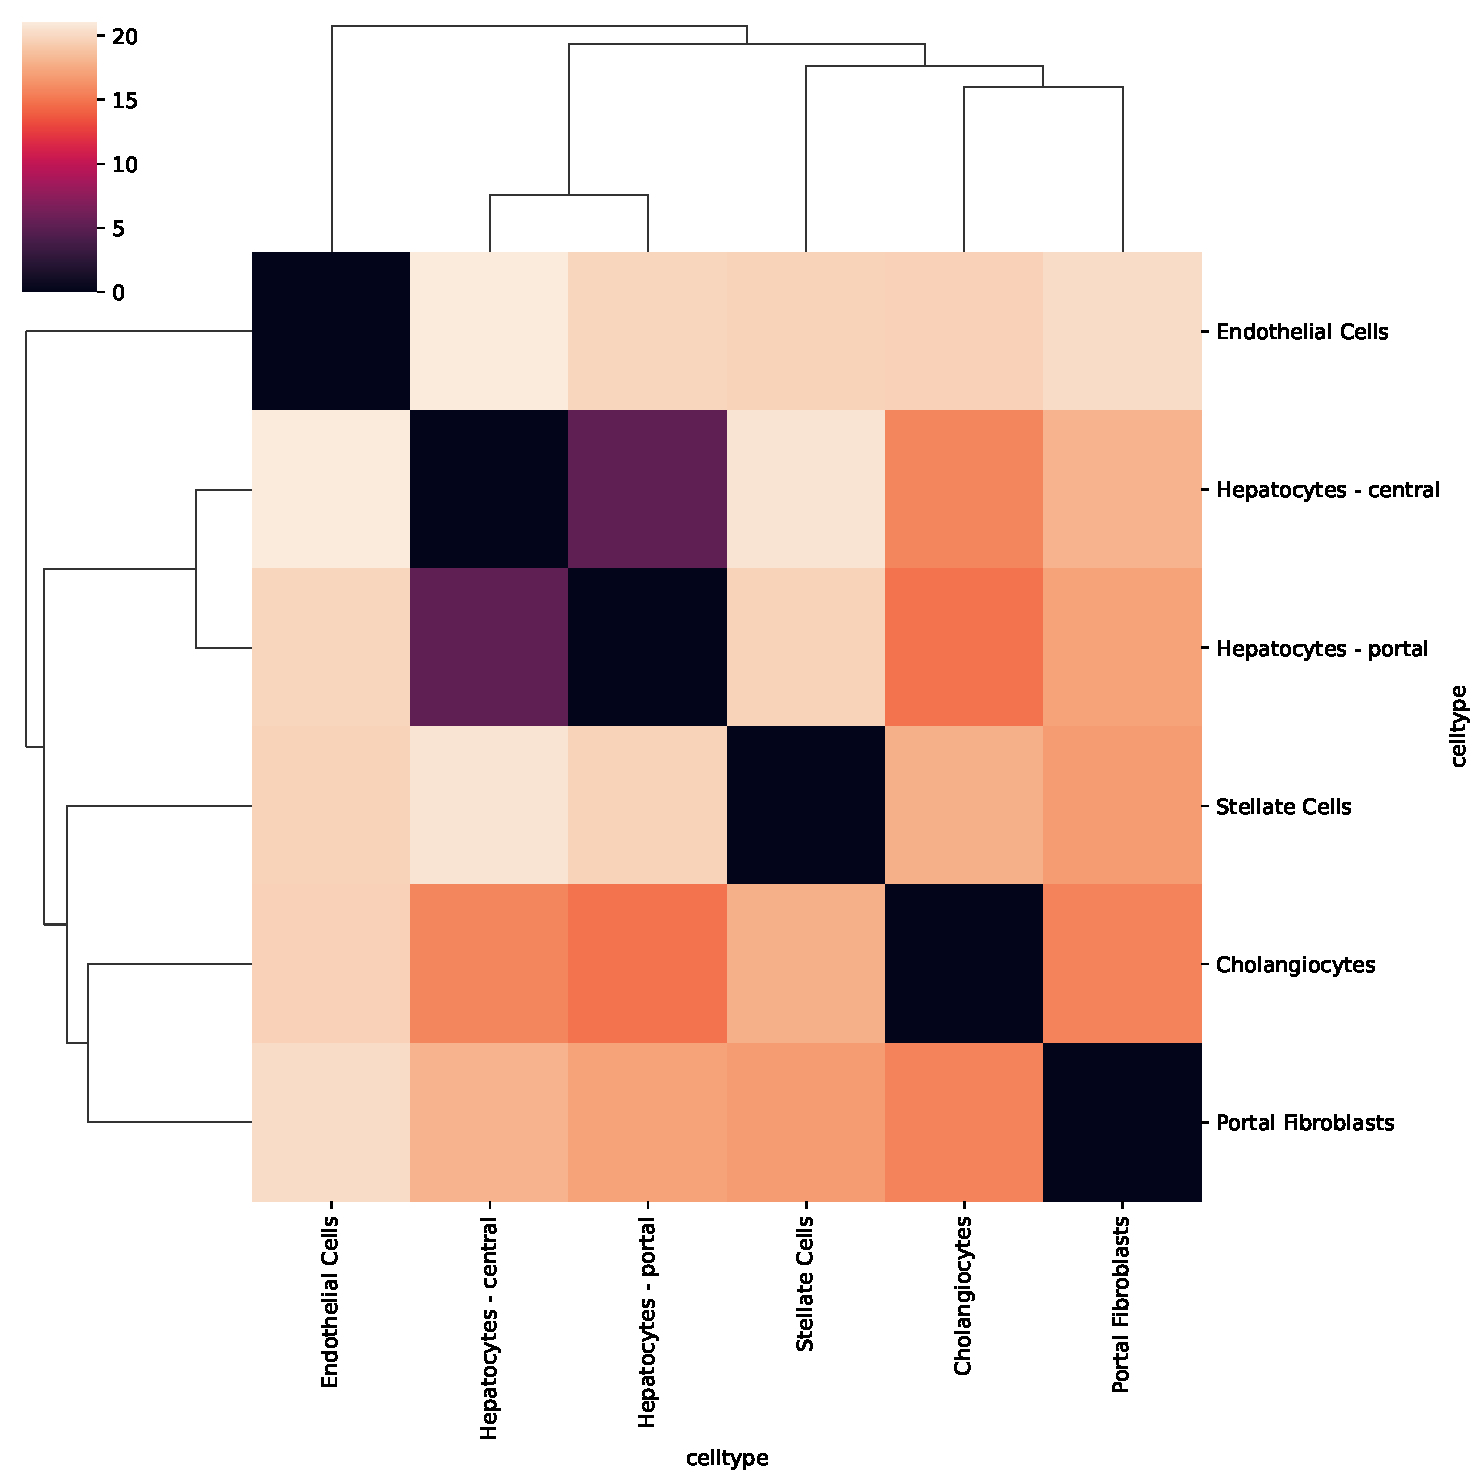
\includegraphics[width=\textwidth]{figures/dose_highest_euclidean_clustermap.pdf}
        \caption{Euclidean}
    \end{minipage}
    \vskip\baselineskip

    \begin{minipage}{0.4\textwidth}
        \centering
        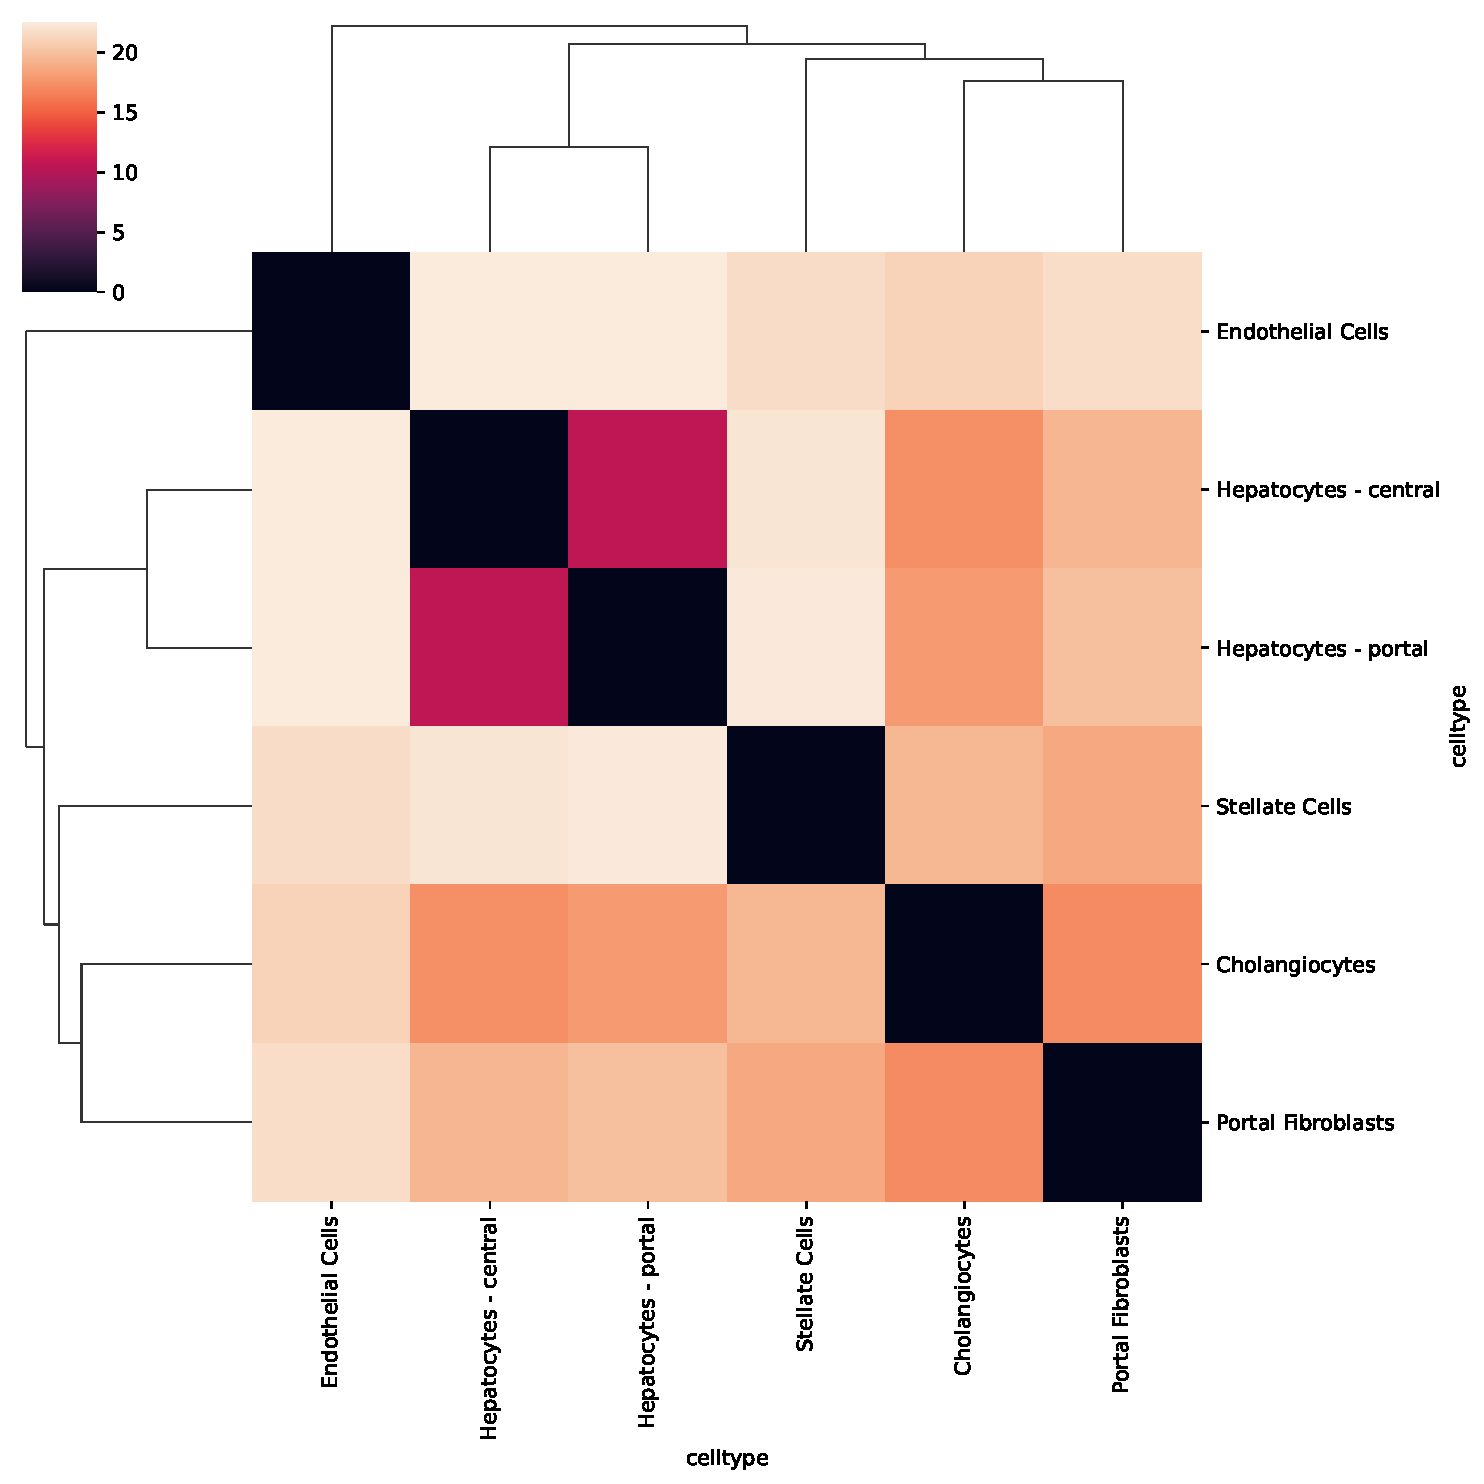
\includegraphics[width=\textwidth]{figures/dose_highest_mean_pairwise_clustermap.pdf}
        \caption{Mean pairwise}
    \end{minipage} \hfill
    \begin{minipage}{0.4\textwidth}
        \centering
        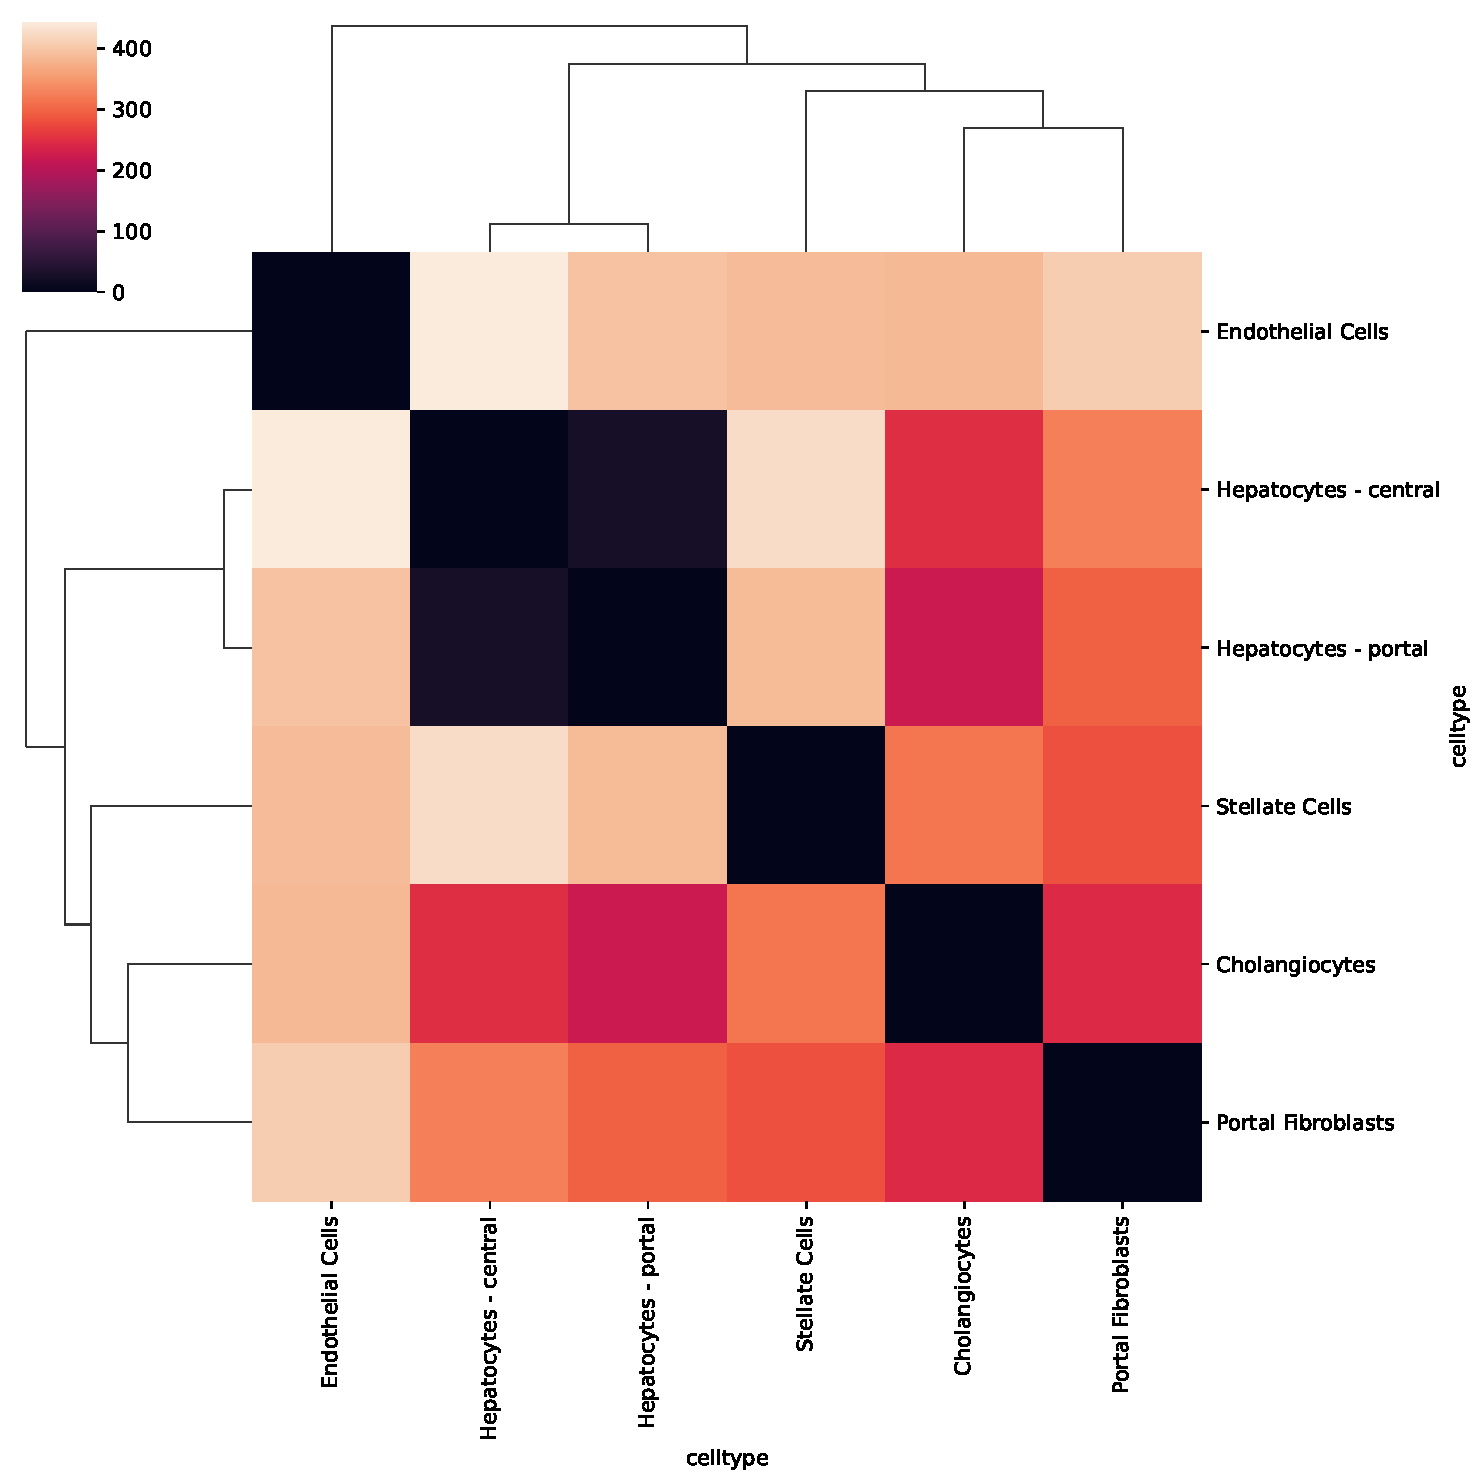
\includegraphics[width=\textwidth]{figures/dose_highest_mmd_clustermap.pdf}
        \caption{MMD}
    \end{minipage}
    \vskip\baselineskip

    \begin{minipage}{0.4\textwidth}
        \centering
        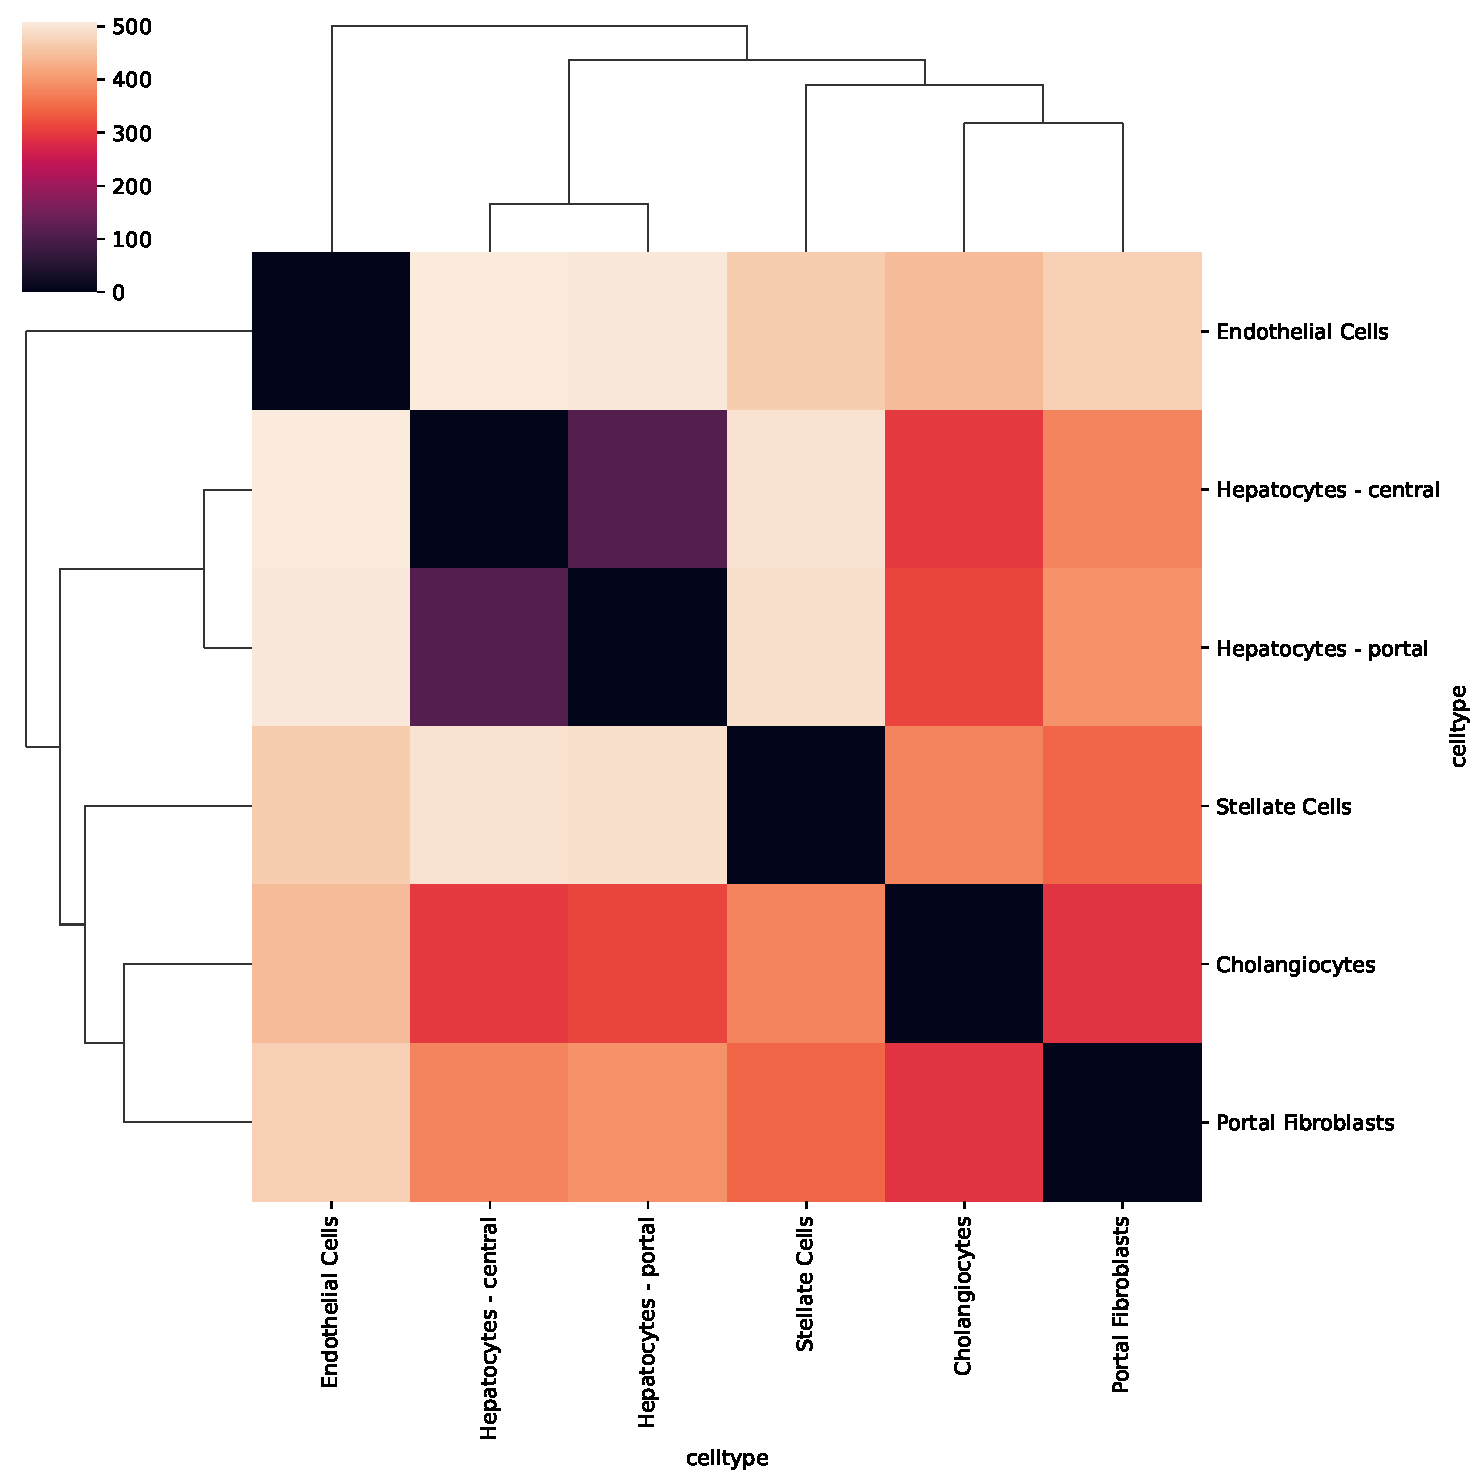
\includegraphics[width=\textwidth]{figures/dose_highest_wasserstein_clustermap.pdf}
        \caption{Wasserstein}
    \end{minipage}
    \caption{Distance metrics for dosage highest 30 $\mu g/kg$ per cell type}
\end{figure}

\begin{figure}
    \centering
    \begin{minipage}{0.4\textwidth}
        \centering
        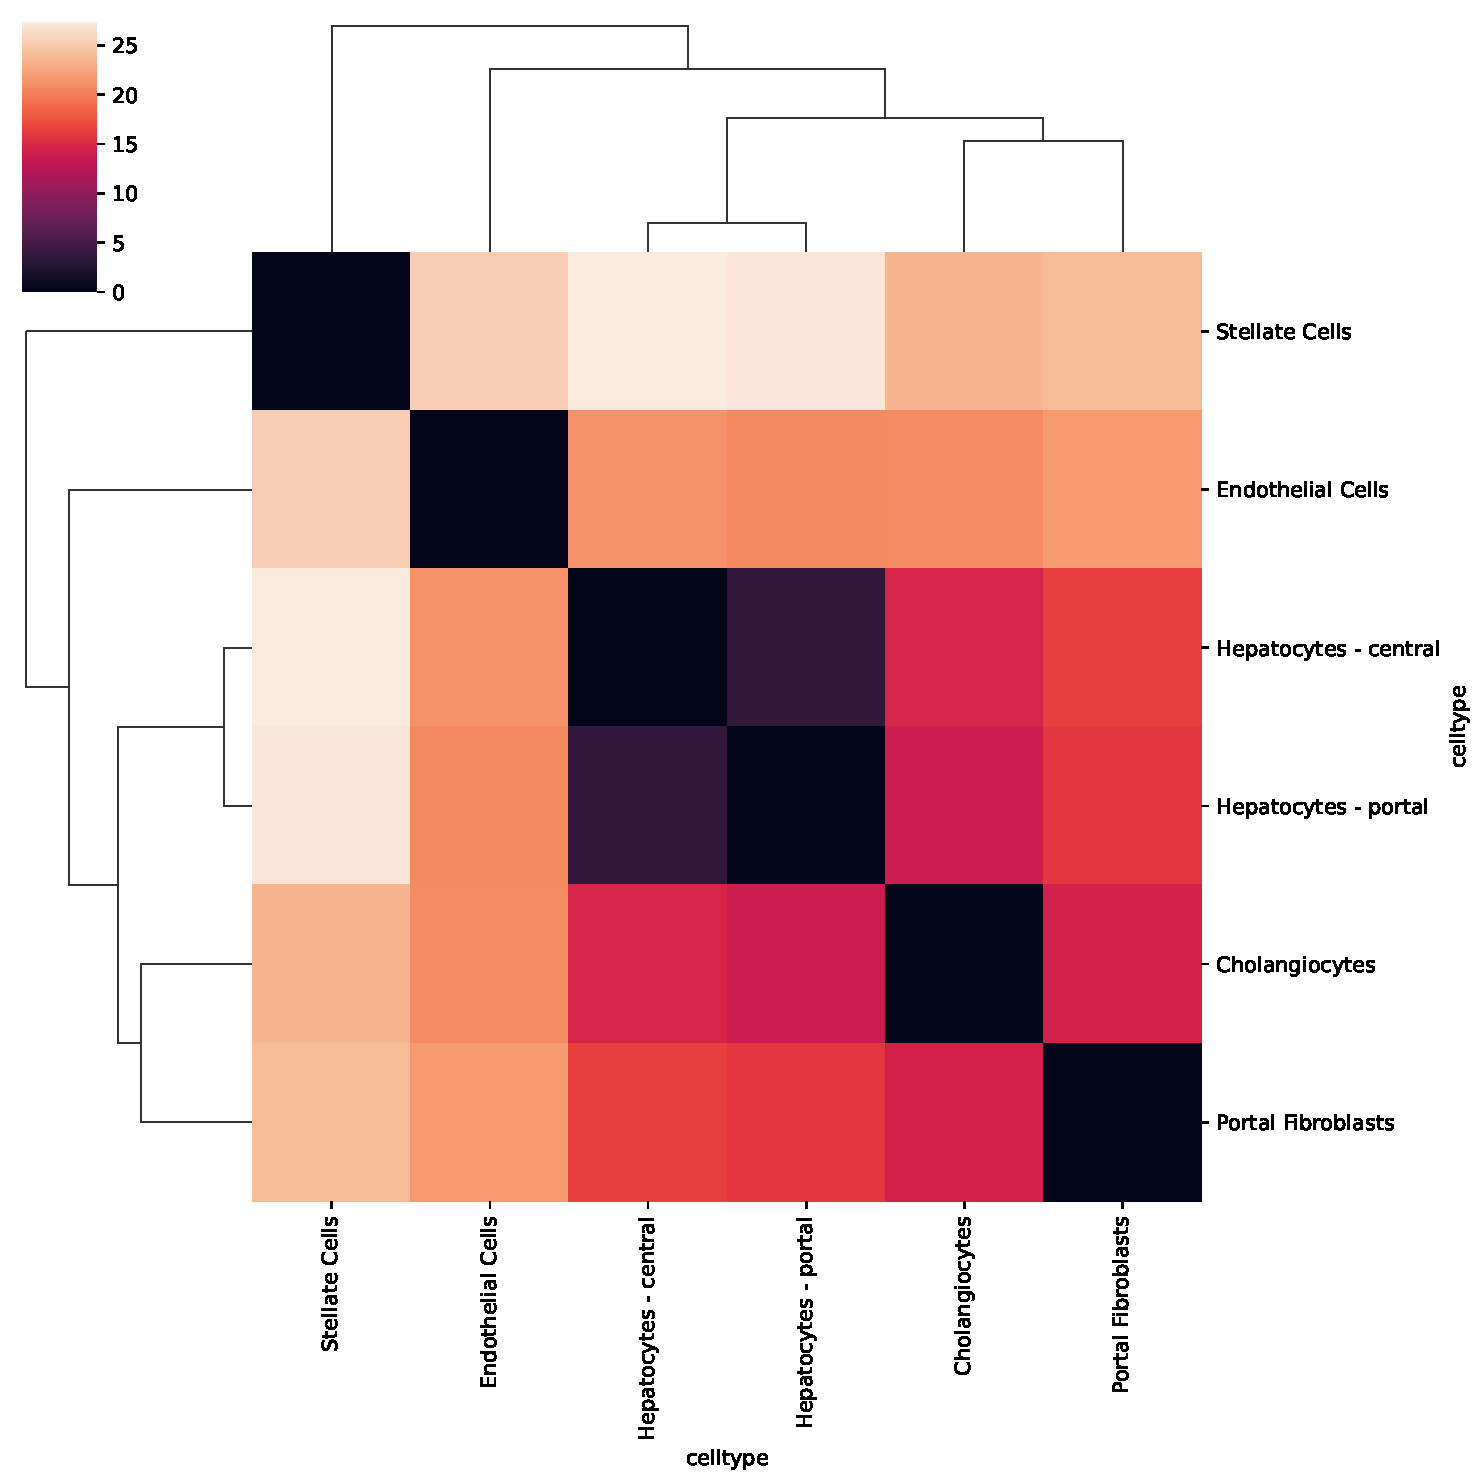
\includegraphics[width=\textwidth]{figures/dose_lowest_edistance_clustermap.pdf}
        \caption{E-distance}
    \end{minipage} \hfill
    \begin{minipage}{0.4\textwidth}
        \centering
        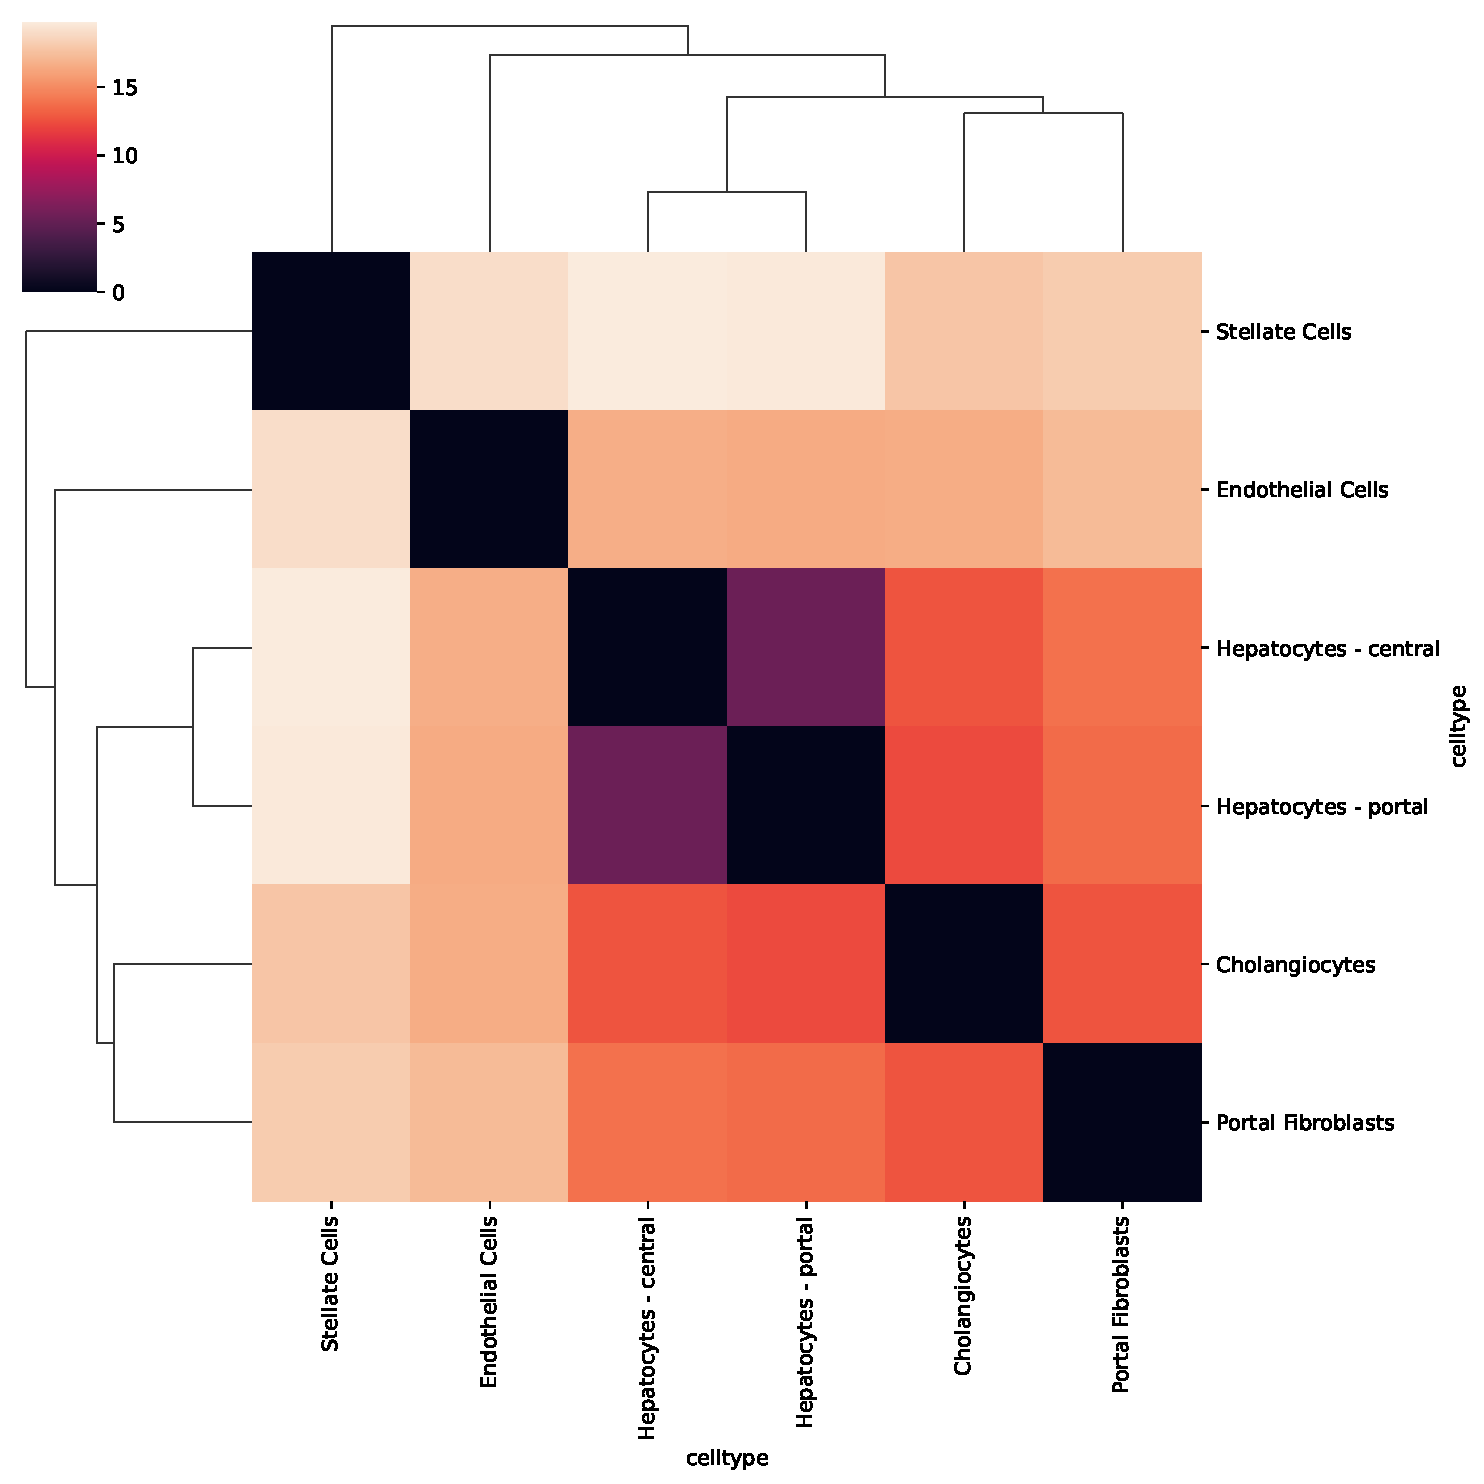
\includegraphics[width=\textwidth]{figures/dose_lowest_euclidean_clustermap.pdf}
        \caption{Euclidean}
    \end{minipage}
    \vskip\baselineskip

    \begin{minipage}{0.4\textwidth}
        \centering
        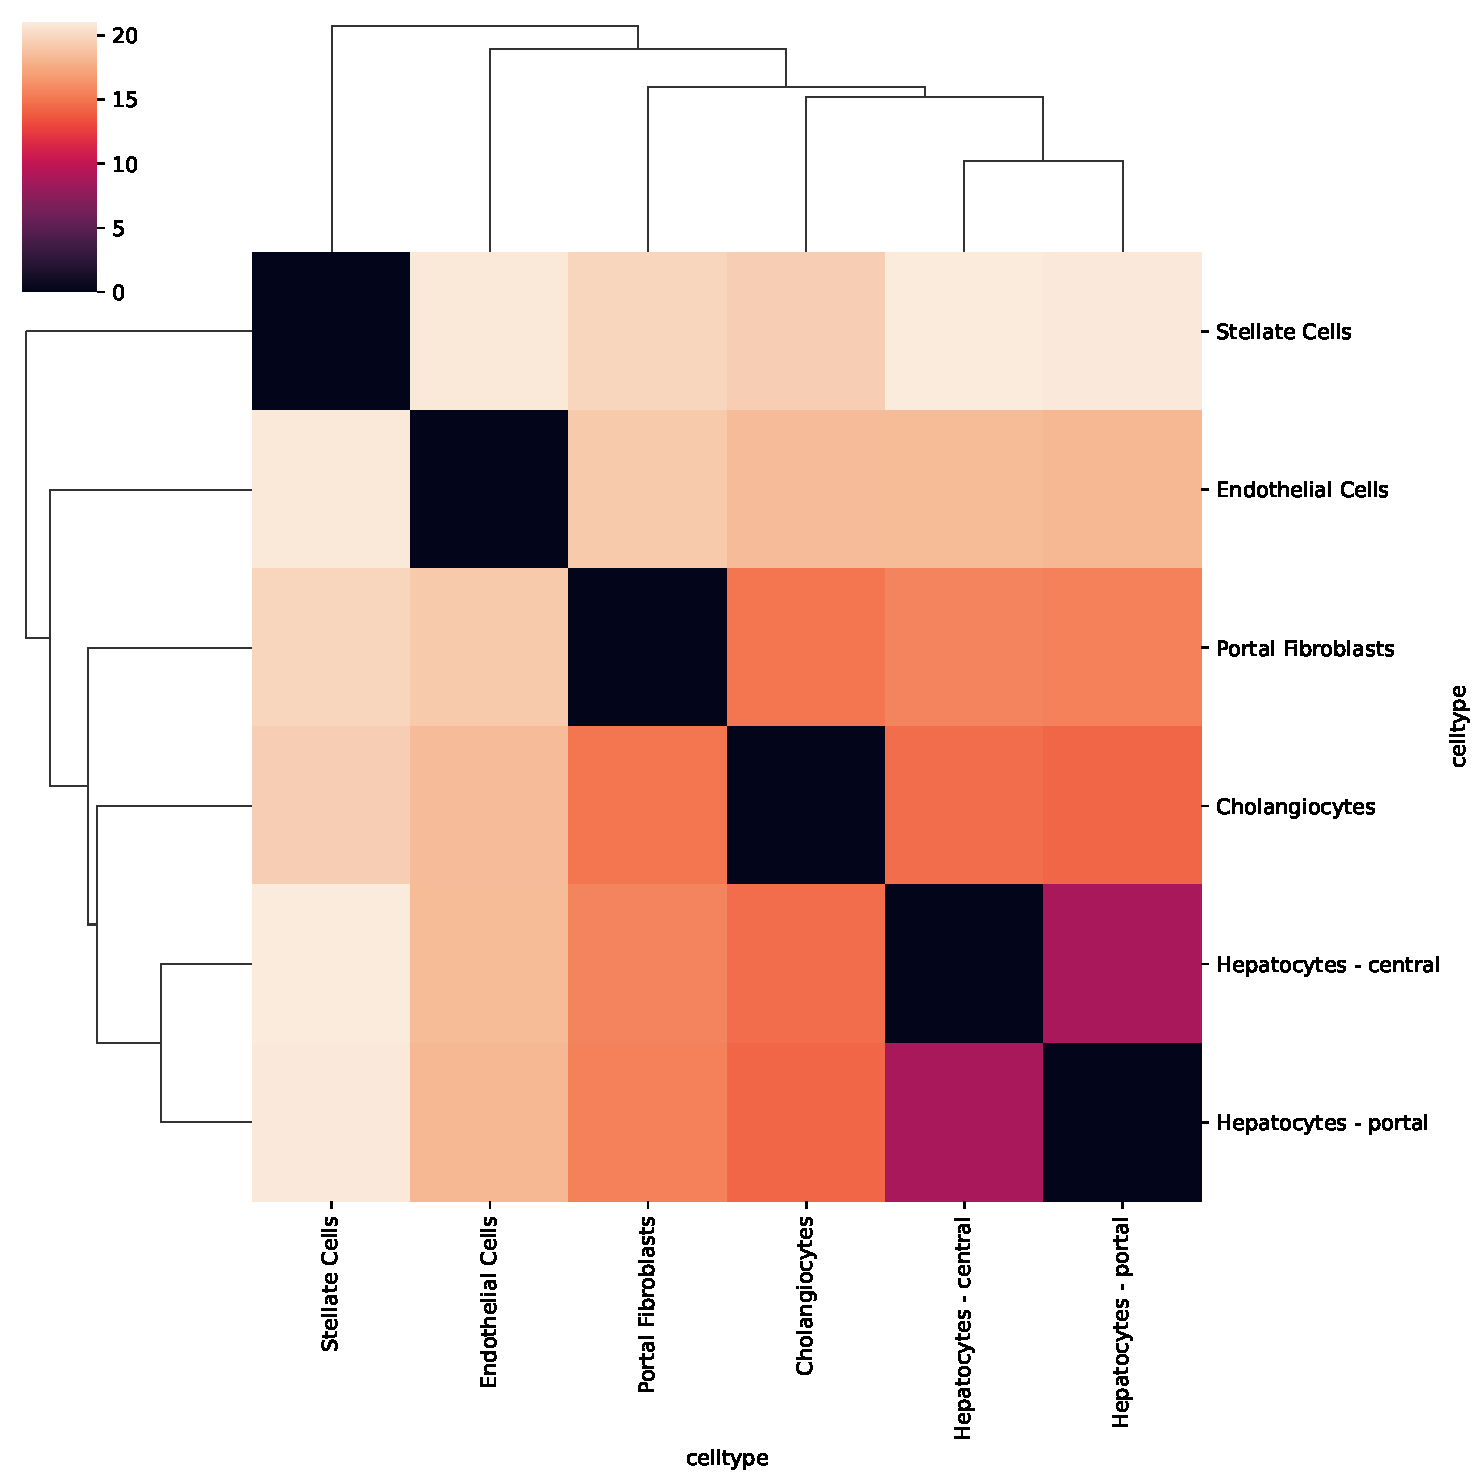
\includegraphics[width=\textwidth]{figures/dose_lowest_mean_pairwise_clustermap.pdf}
        \caption{Mean pairwise}
    \end{minipage} \hfill
    \begin{minipage}{0.4\textwidth}
        \centering
        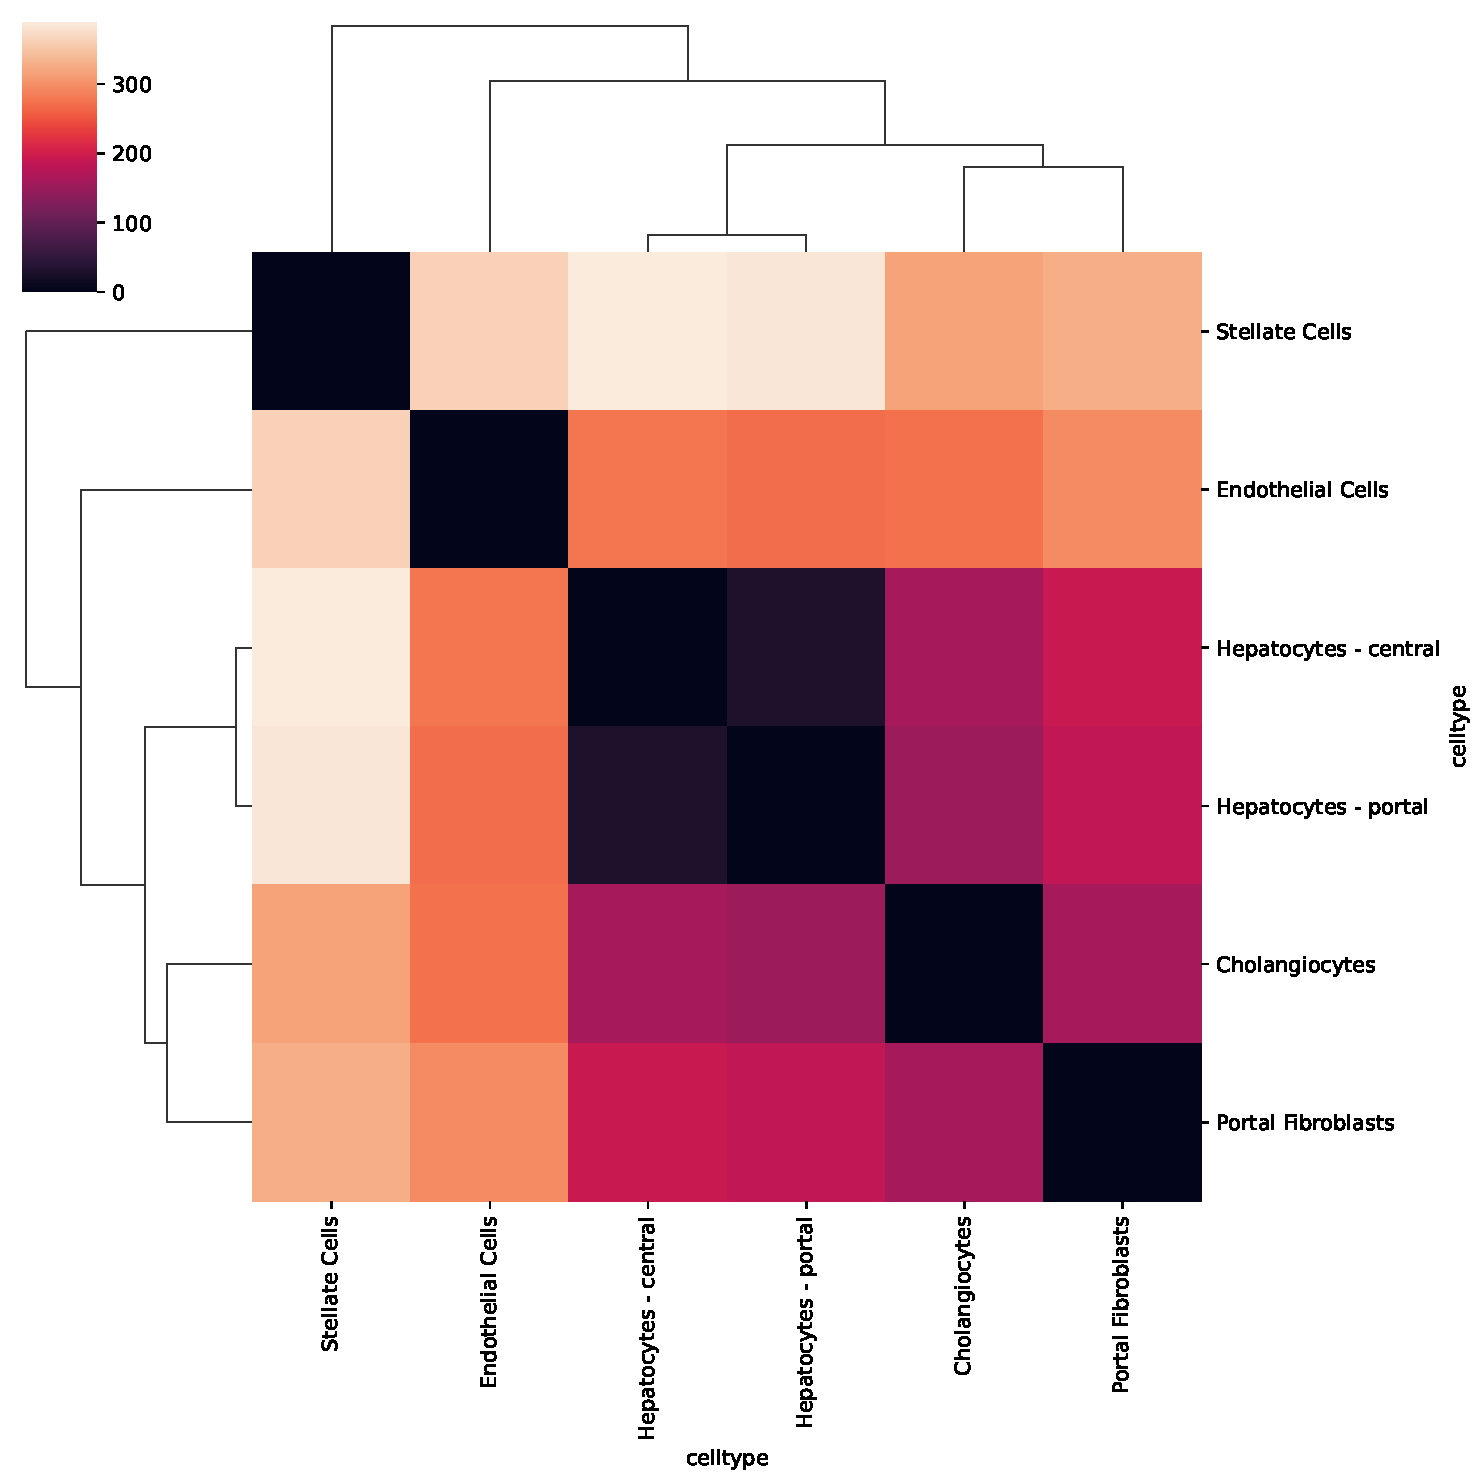
\includegraphics[width=\textwidth]{figures/dose_lowest_mmd_clustermap.pdf}
        \caption{MMD}
    \end{minipage}
    \vskip\baselineskip

    \begin{minipage}{0.4\textwidth}
        \centering
        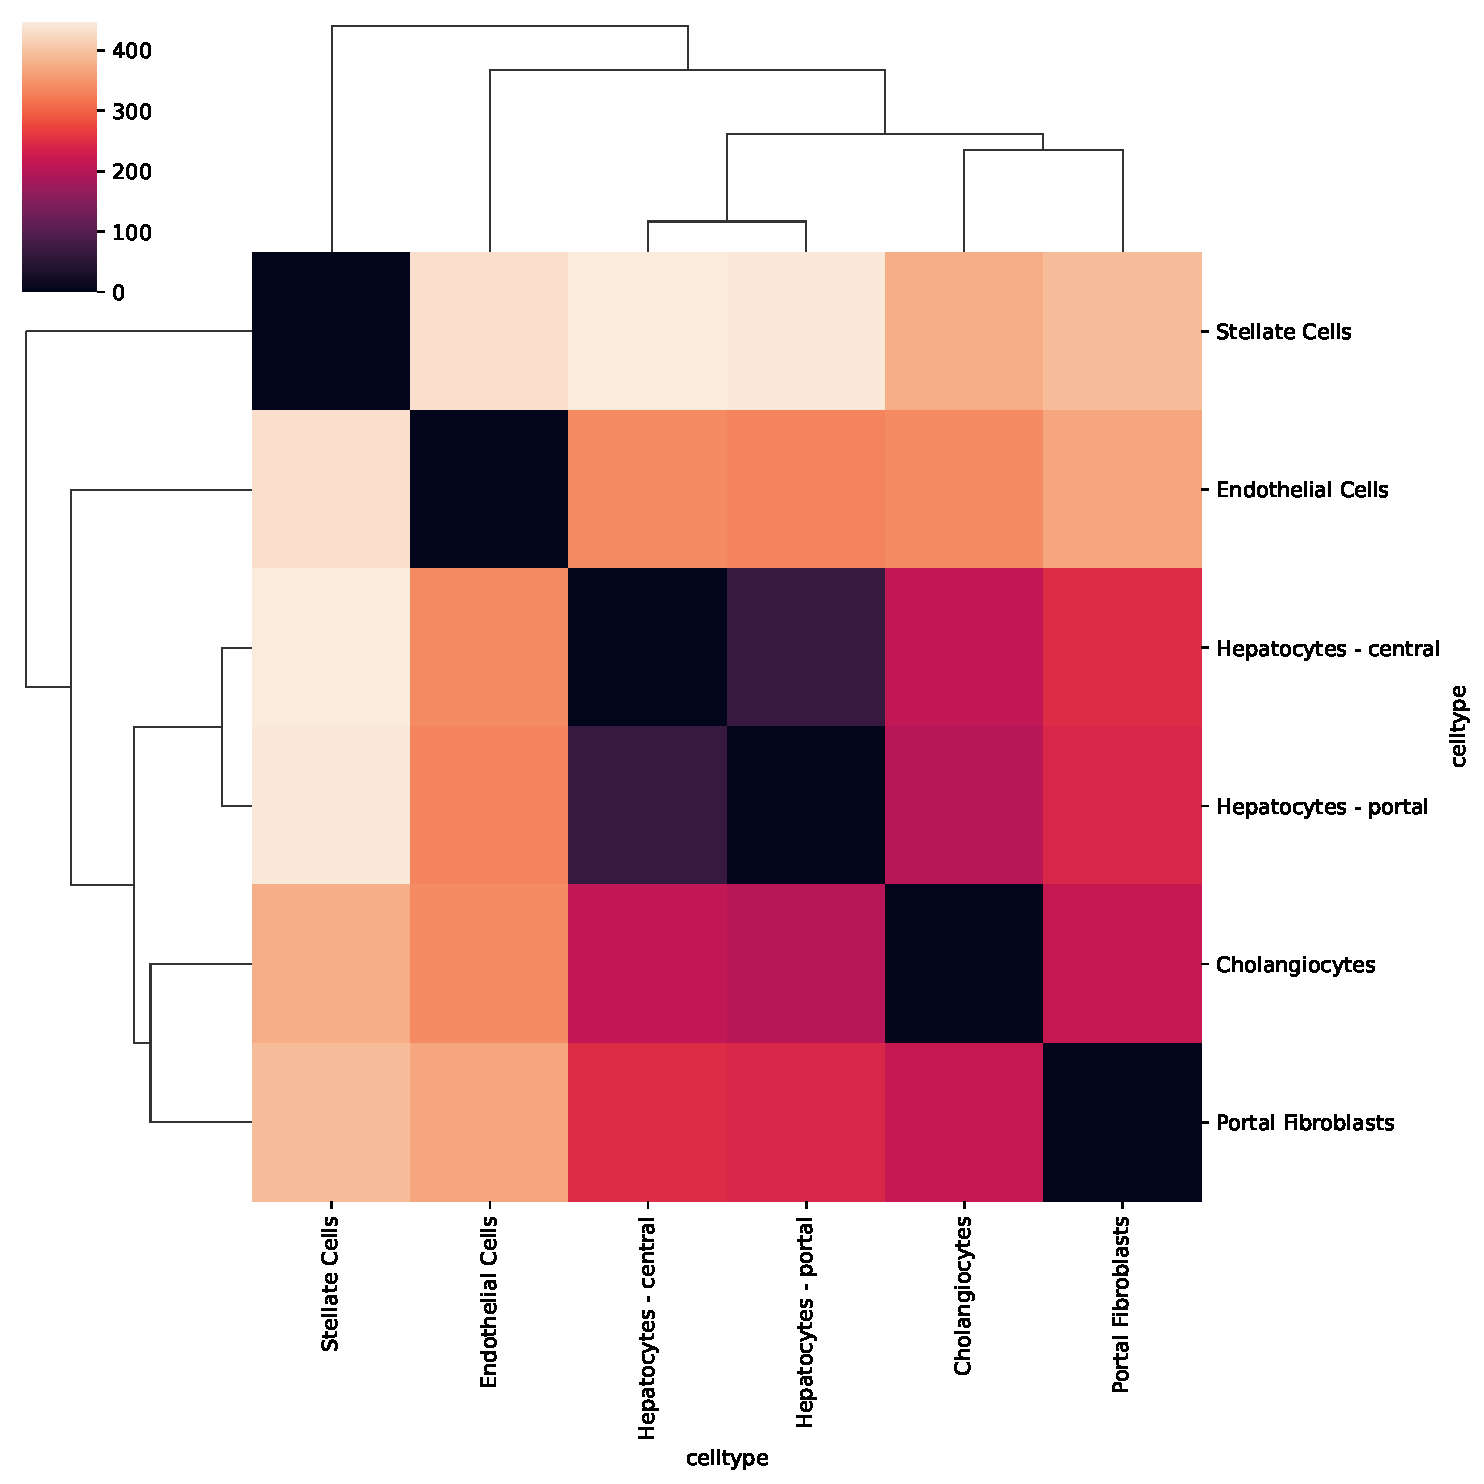
\includegraphics[width=\textwidth]{figures/dose_lowest_wasserstein_clustermap.pdf}
        \caption{Wasserstein}
    \end{minipage}
    \caption{Distance metrics for lowest dosage 0.01 $\mu g/kg$ per cell type}
\end{figure}

\clearpage


\subsection{PBMC dataset}


\begin{figure}[h]
    \centering
    \begin{subfigure}[t]{0.49\textwidth}
        \centering
        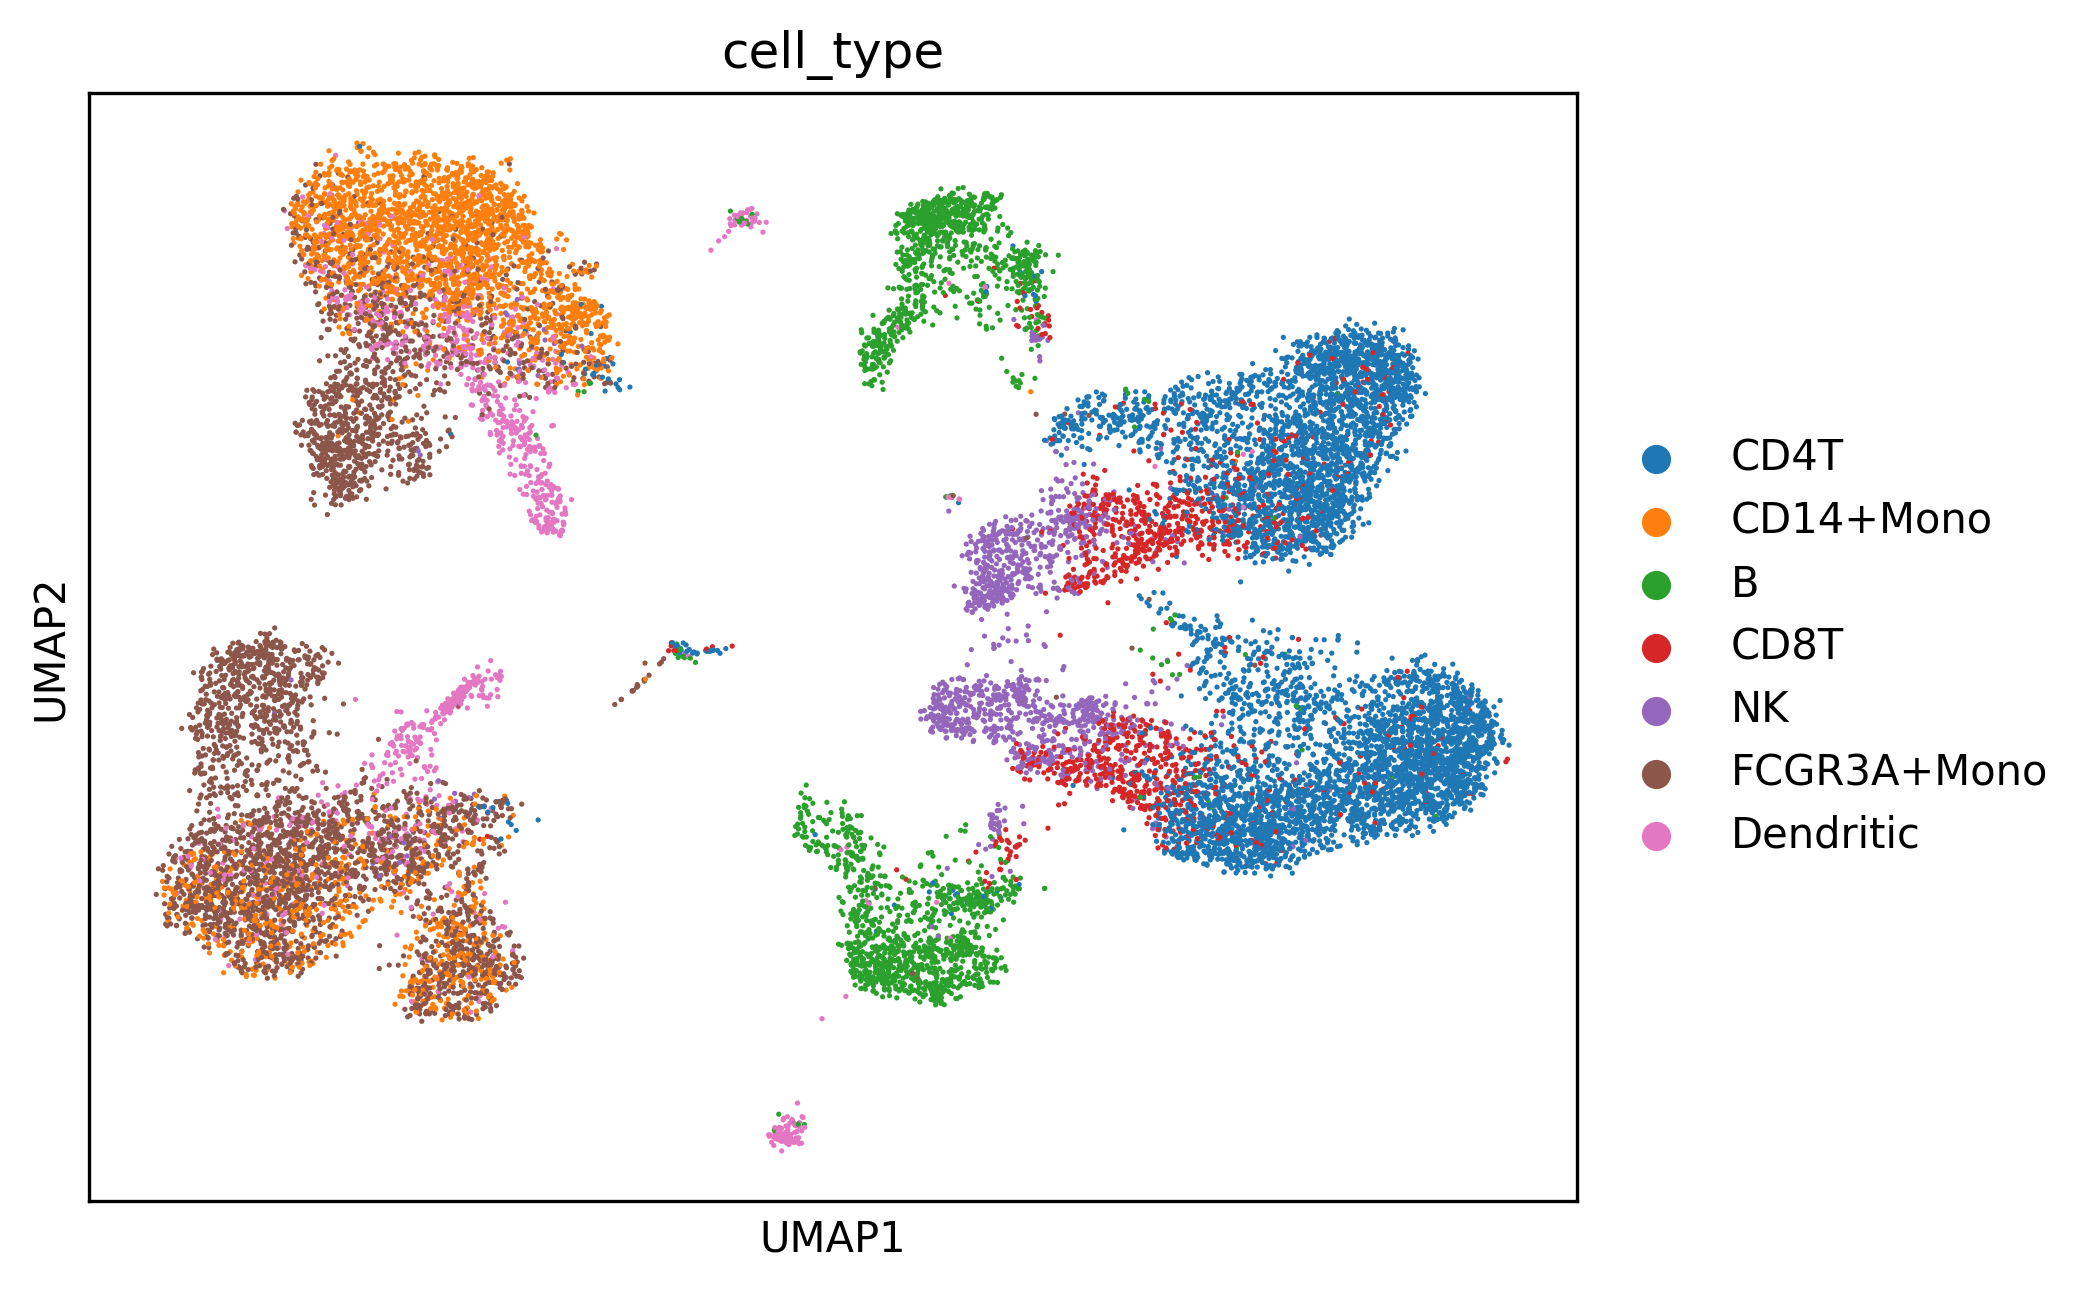
\includegraphics[width=\textwidth]{figures/pbmc_cell_umap.png}
        \caption{}
        \label{fig:figure1}
    \end{subfigure}
    \hfill
    \begin{subfigure}[t]{0.49\textwidth}
        \centering
        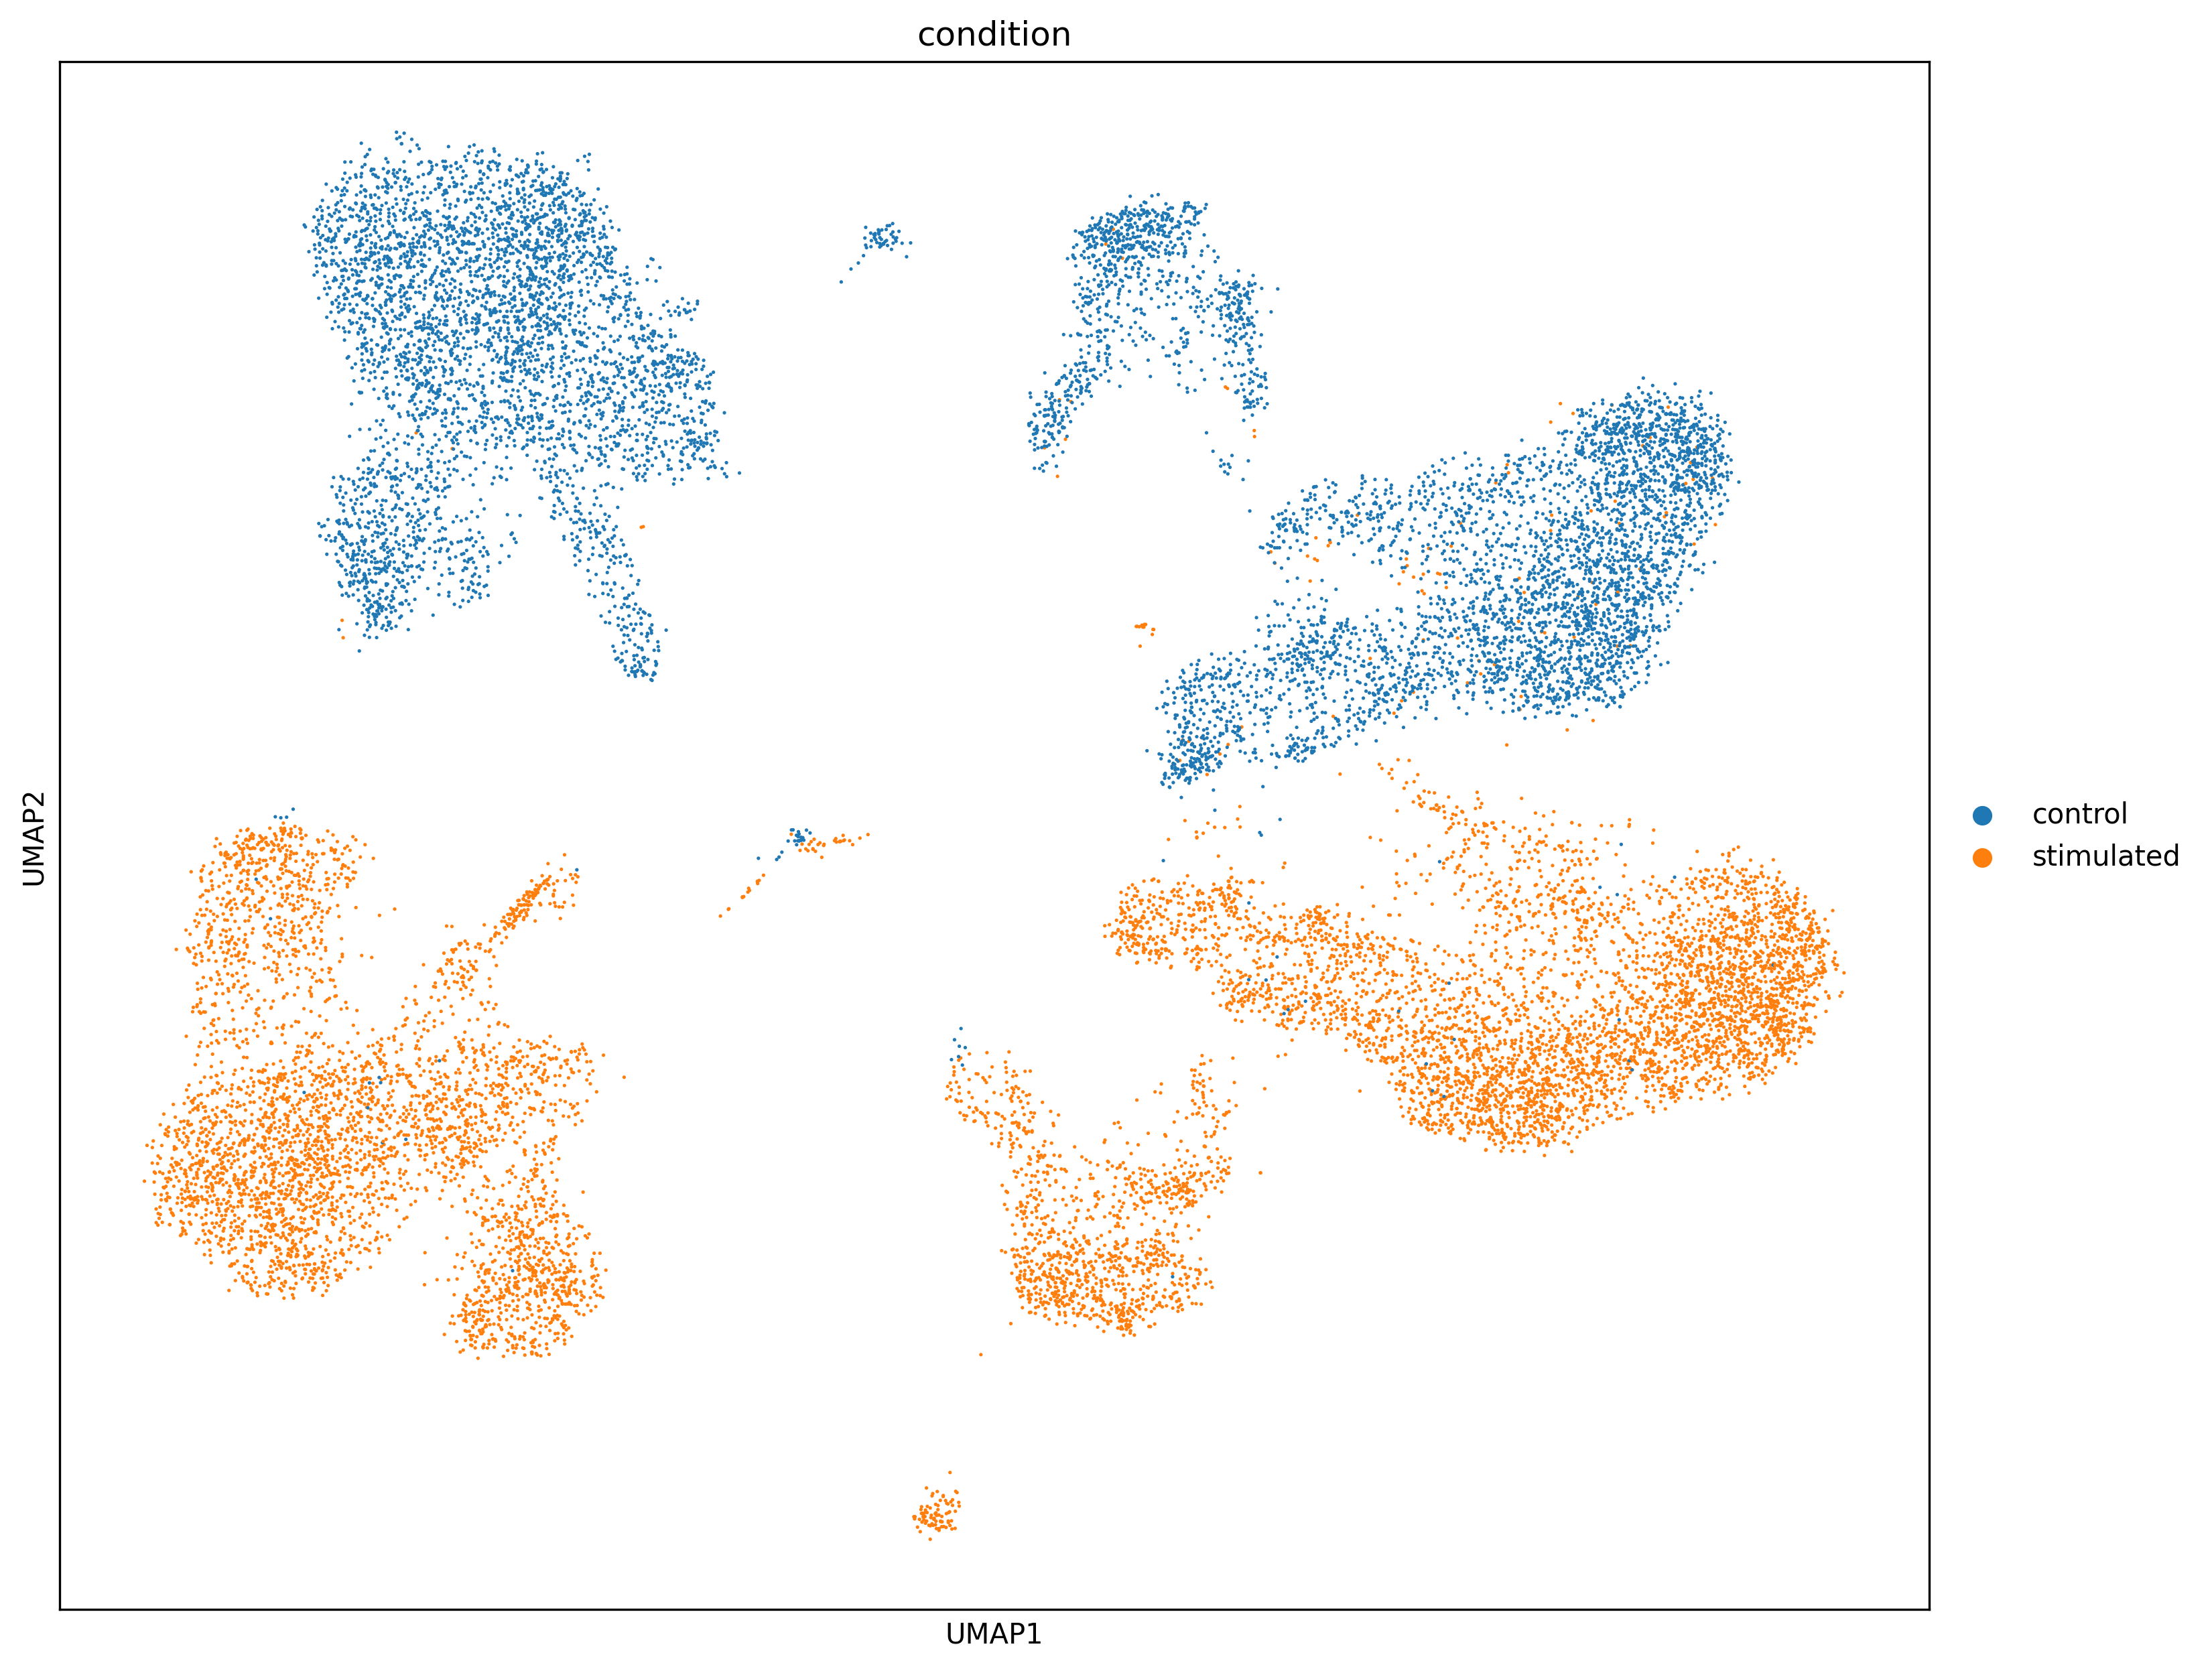
\includegraphics[width=.95\textwidth]{figures/pbmc_condtion_umap.png}
        \caption{}
        \label{fig:figure2}
    \end{subfigure}
    \hfill
    \begin{subfigure}[b]{\textwidth}
        \centering
        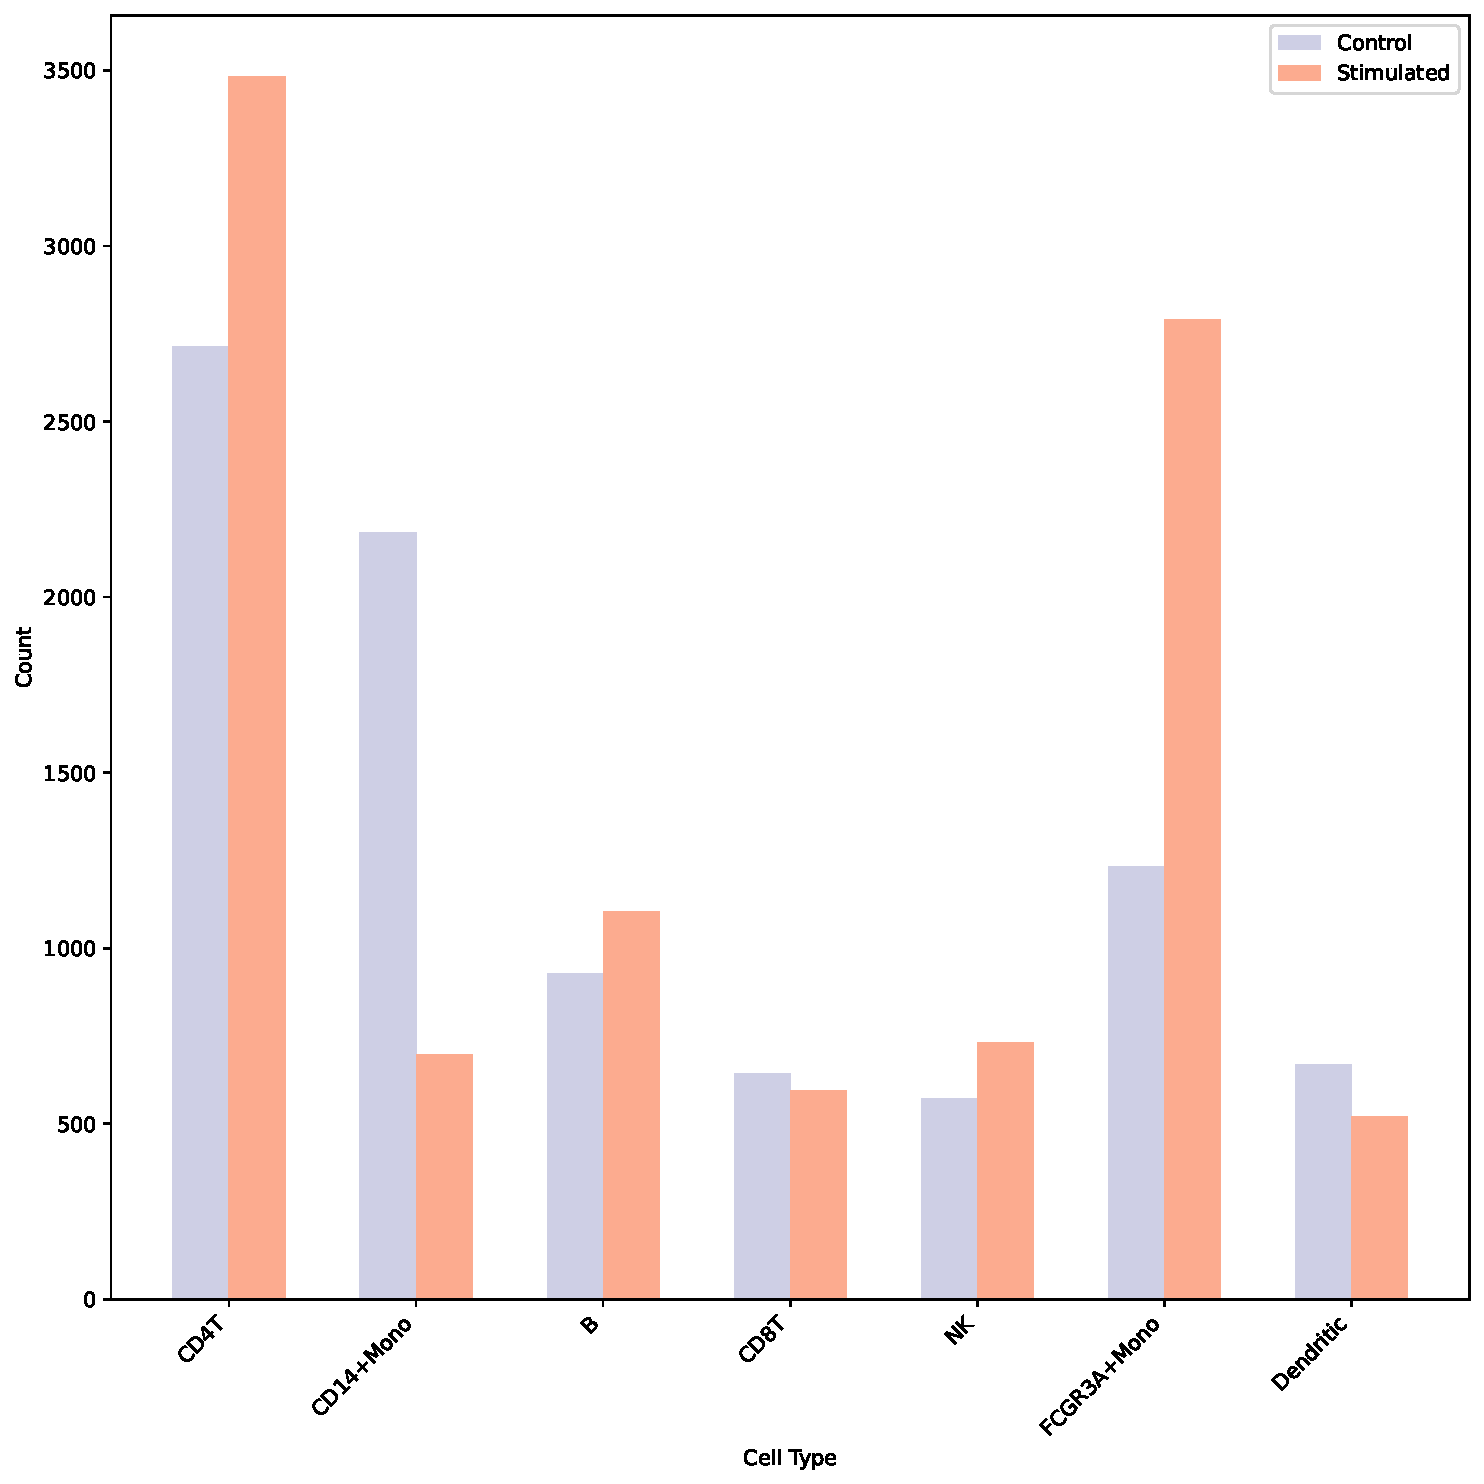
\includegraphics[width=.6\textwidth]{figures/pbmc_counts.pdf}
        \caption{}
        \label{fig:figure3}
    \end{subfigure}
    \caption{PBMC overview}
    \label{fig:combined}
\end{figure}

\clearpage

\begin{figure}
    \centering
    \begin{minipage}{0.4\textwidth}
        \centering
        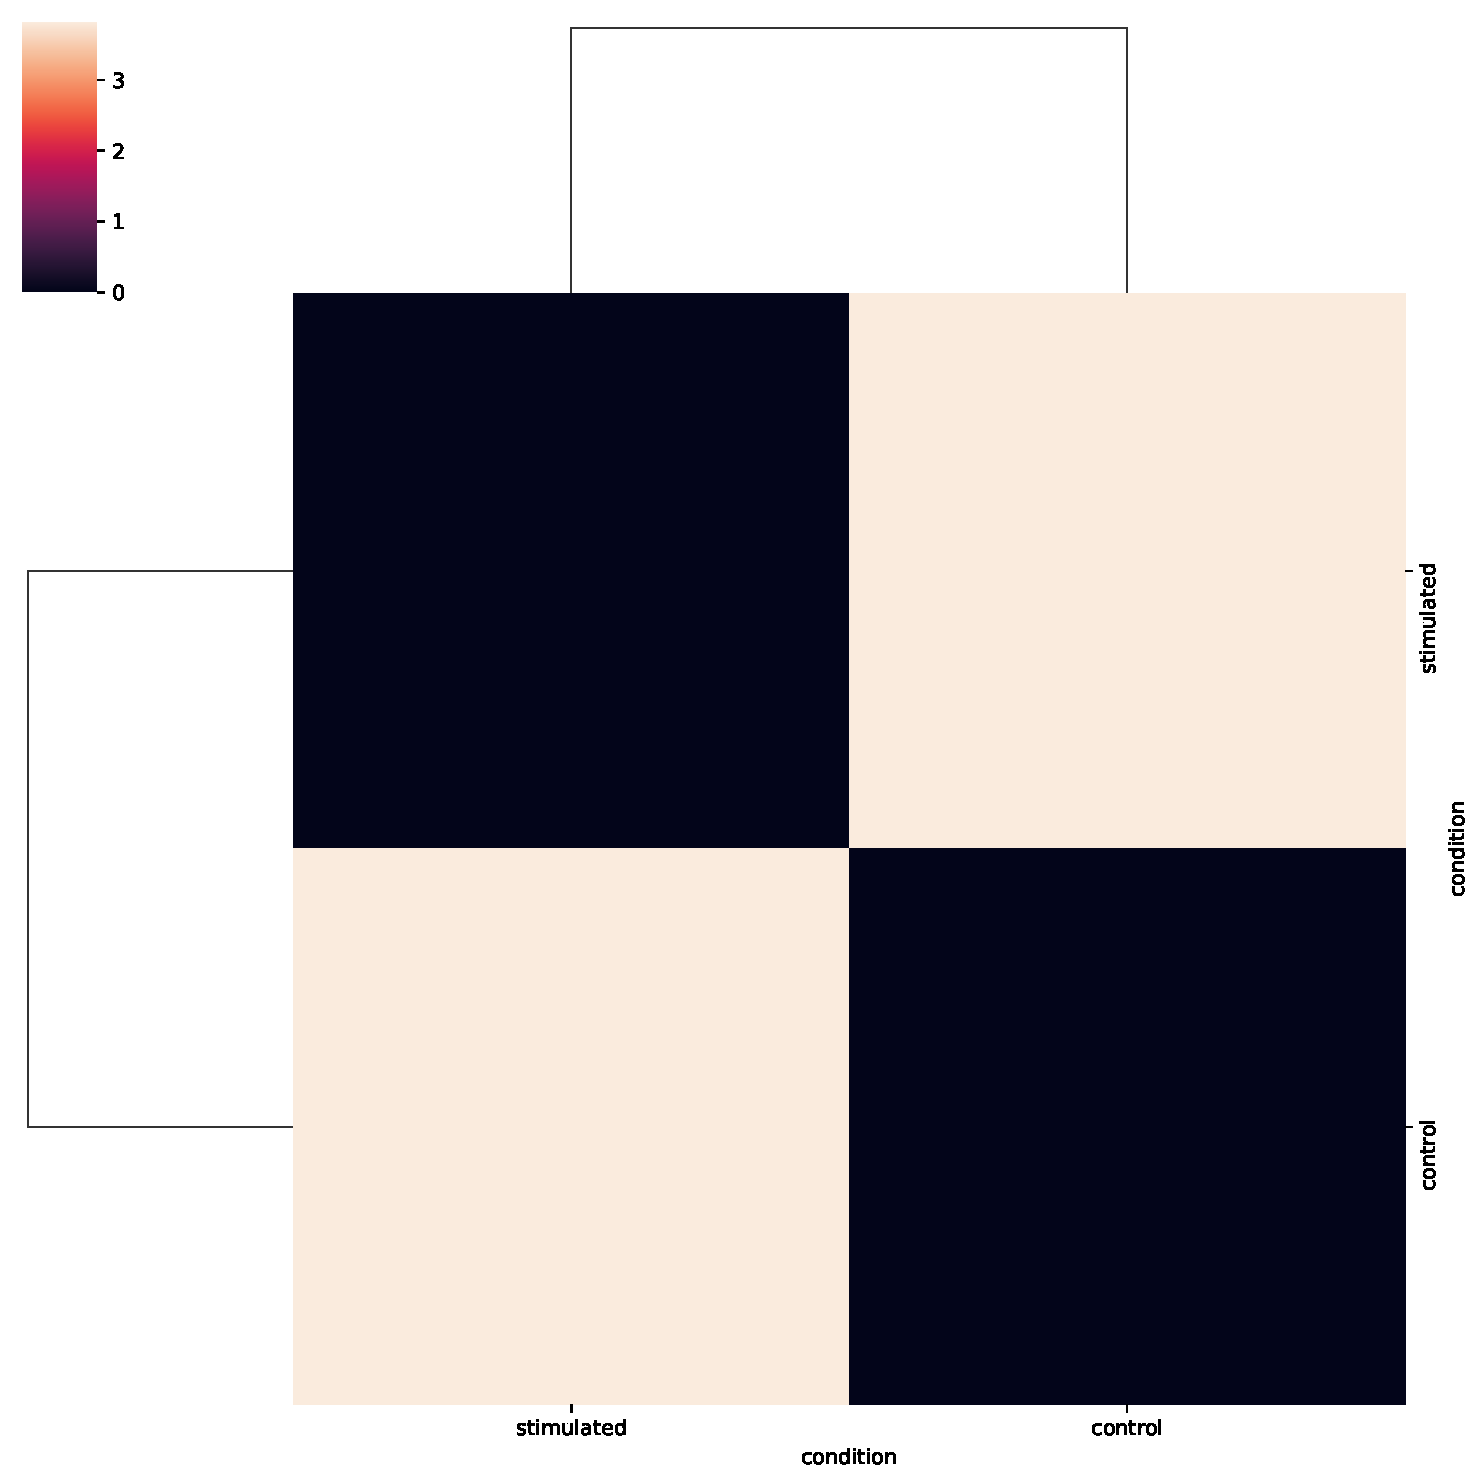
\includegraphics[width=\textwidth]{figures/pbmc_condition_edistance_clustermap.pdf}
        \caption{E-distance}
    \end{minipage} \hfill
    \begin{minipage}{0.4\textwidth}
        \centering
        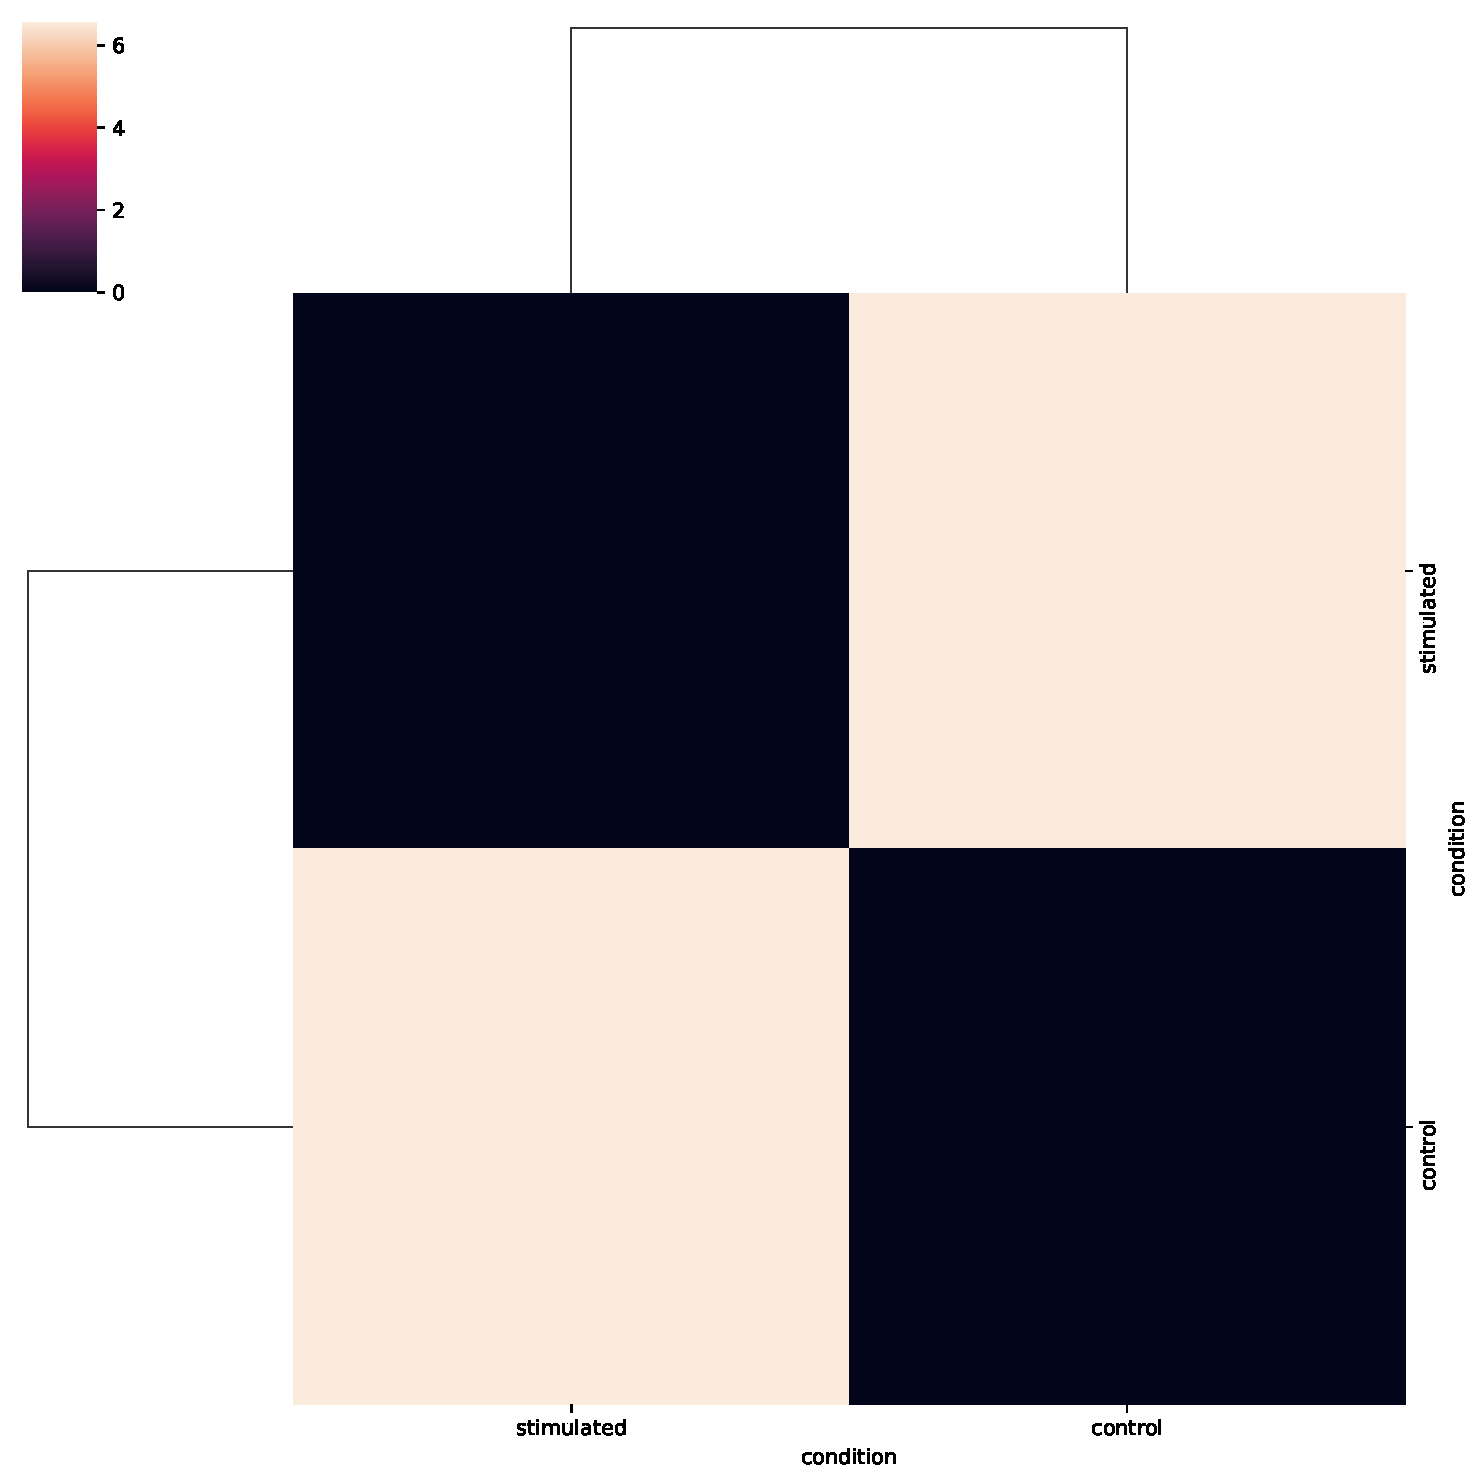
\includegraphics[width=\textwidth]{figures/pbmc_condition_euclidean_clustermap.pdf}
        \caption{Euclidean}
    \end{minipage}
    \vskip\baselineskip

    \begin{minipage}{0.4\textwidth}
        \centering
        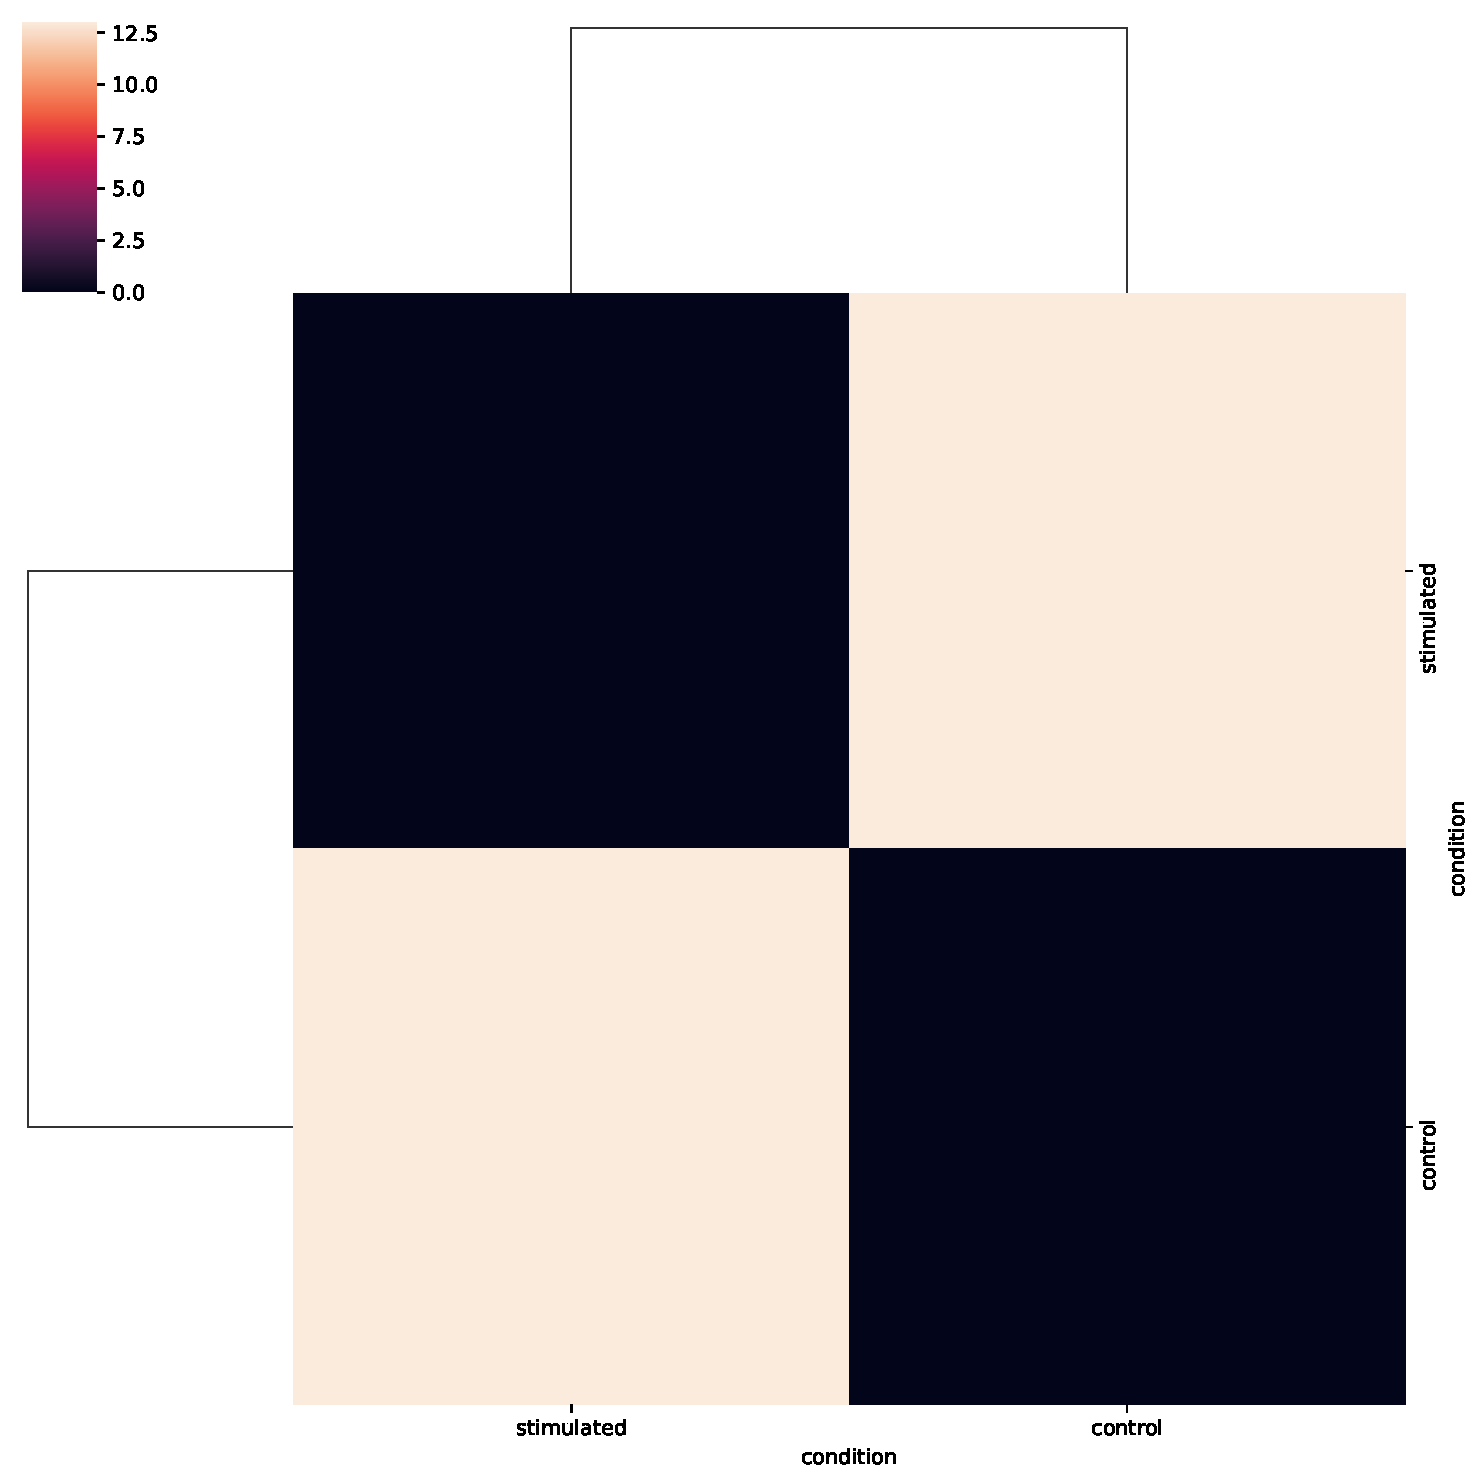
\includegraphics[width=\textwidth]{figures/pbmc_condition_mean_pairwise_clustermap.pdf}
        \caption{Mean pairwise}
    \end{minipage} \hfill
    \begin{minipage}{0.4\textwidth}
        \centering
        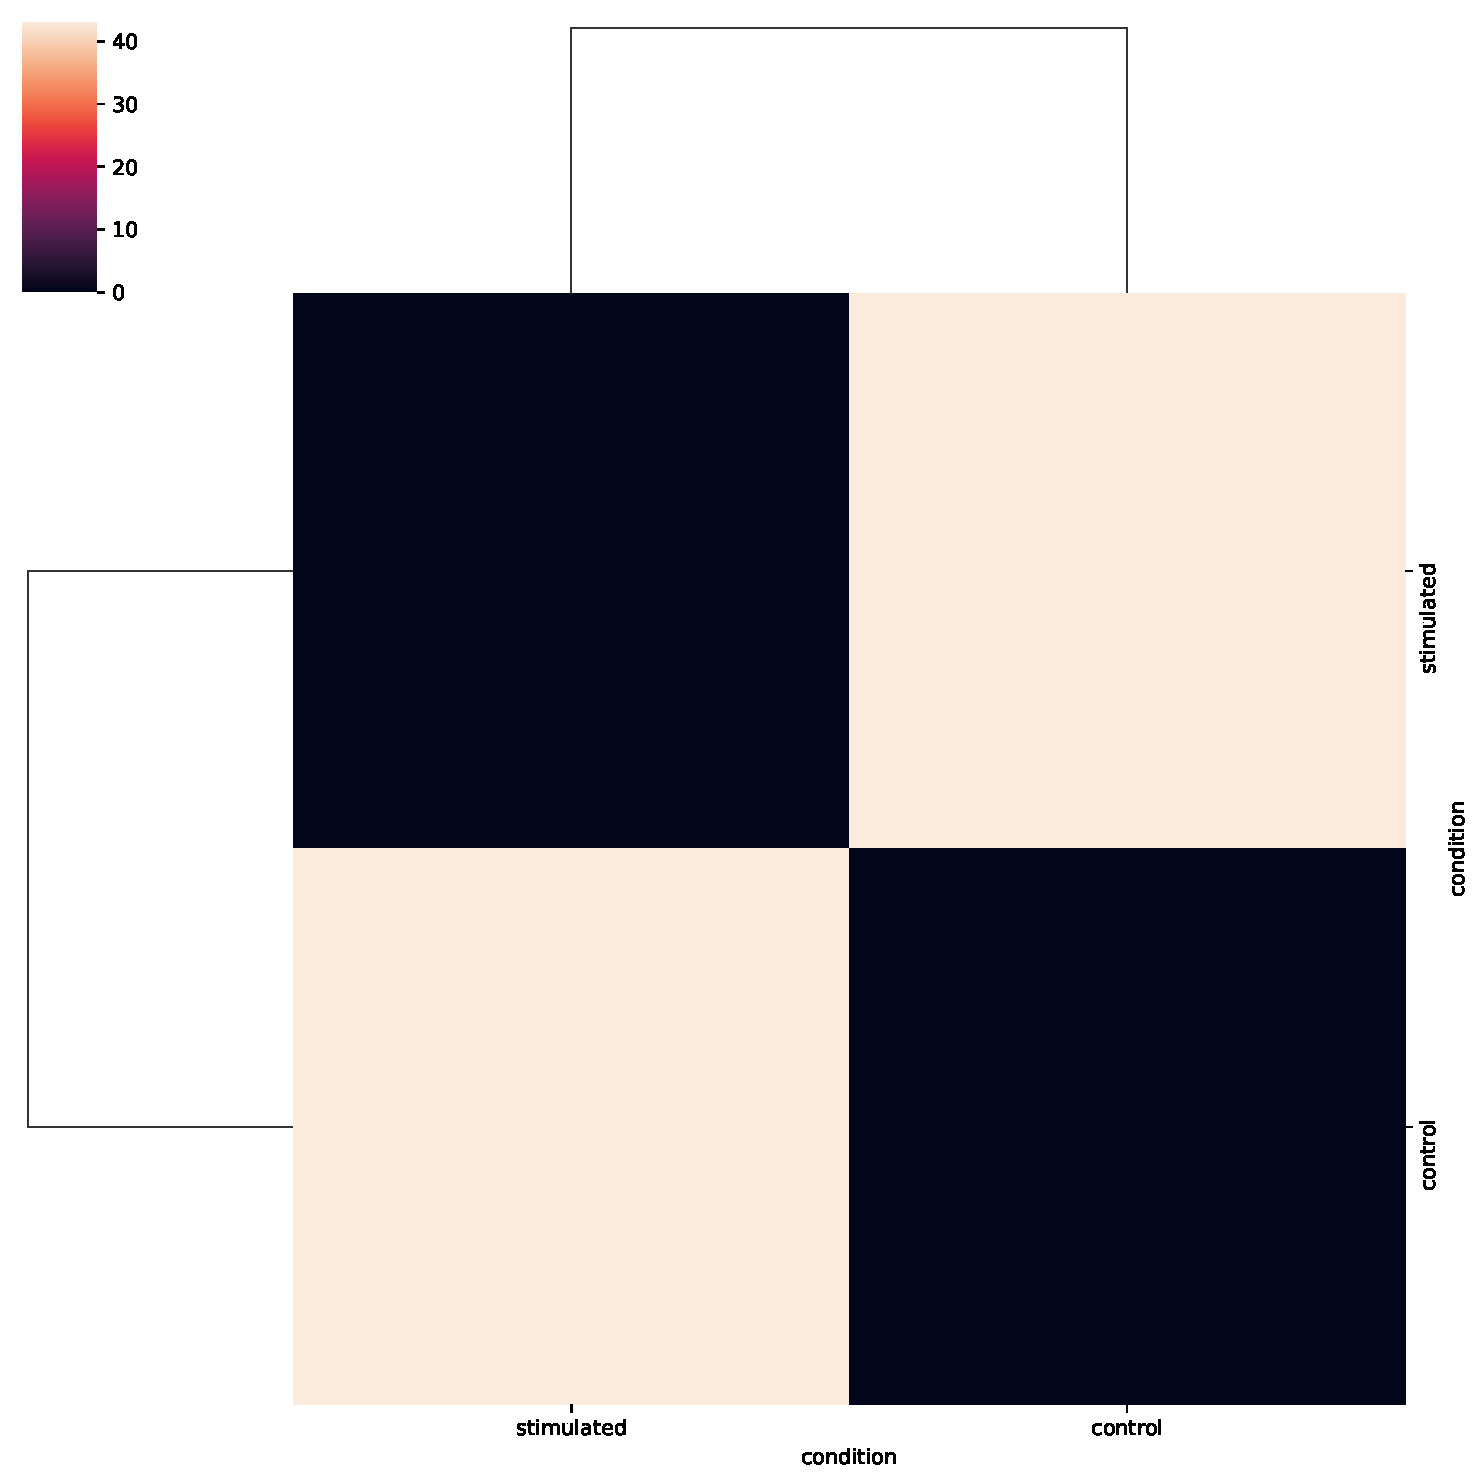
\includegraphics[width=\textwidth]{figures/pbmc_condition_mmd_clustermap.pdf}
        \caption{MMD}
    \end{minipage}
    \vskip\baselineskip

    \begin{minipage}{0.4\textwidth}
        \centering
        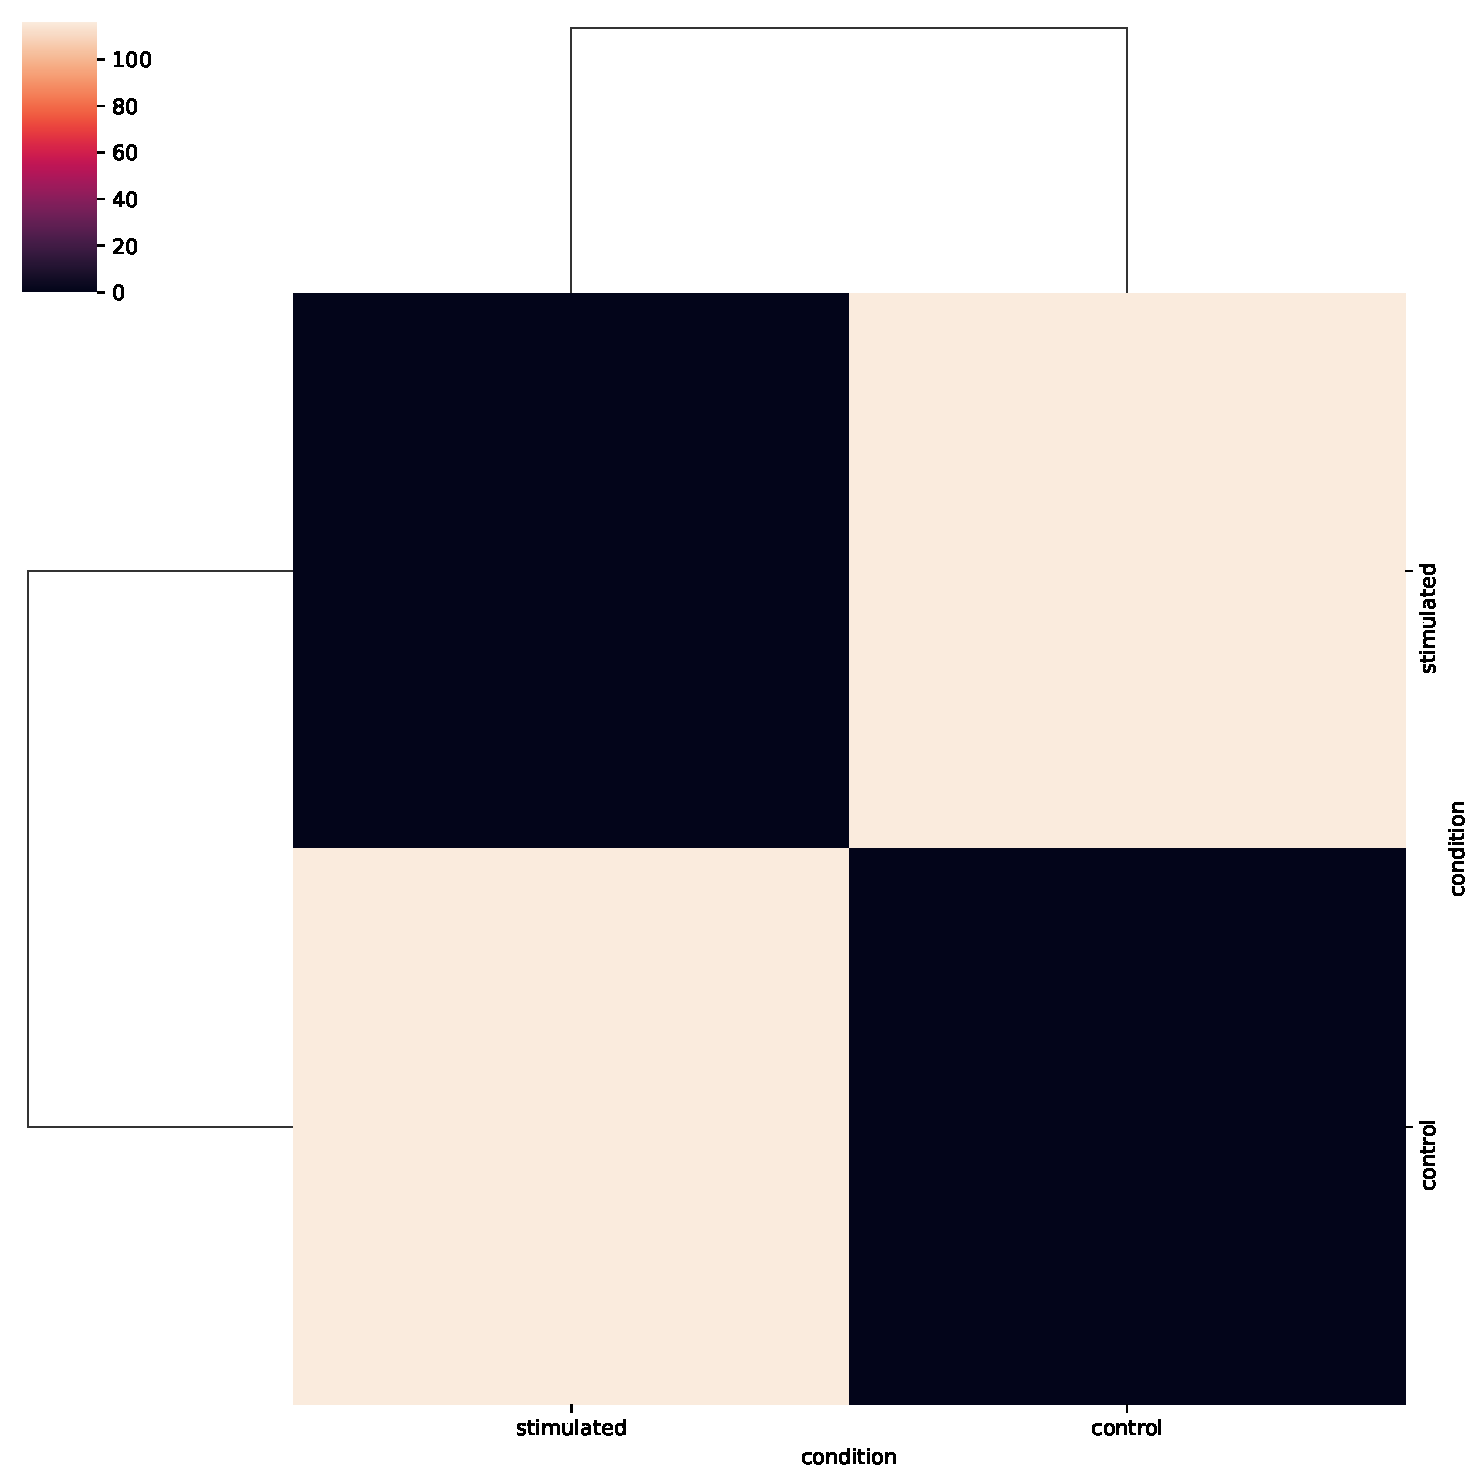
\includegraphics[width=\textwidth]{figures/pbmc_condition_wasserstein_clustermap.pdf}
        \caption{Wasserstein}
    \end{minipage}
    \caption{Distance metrics per condition}
\end{figure}

\clearpage


\begin{figure}
    \centering
    \begin{minipage}{0.4\textwidth}
        \centering
        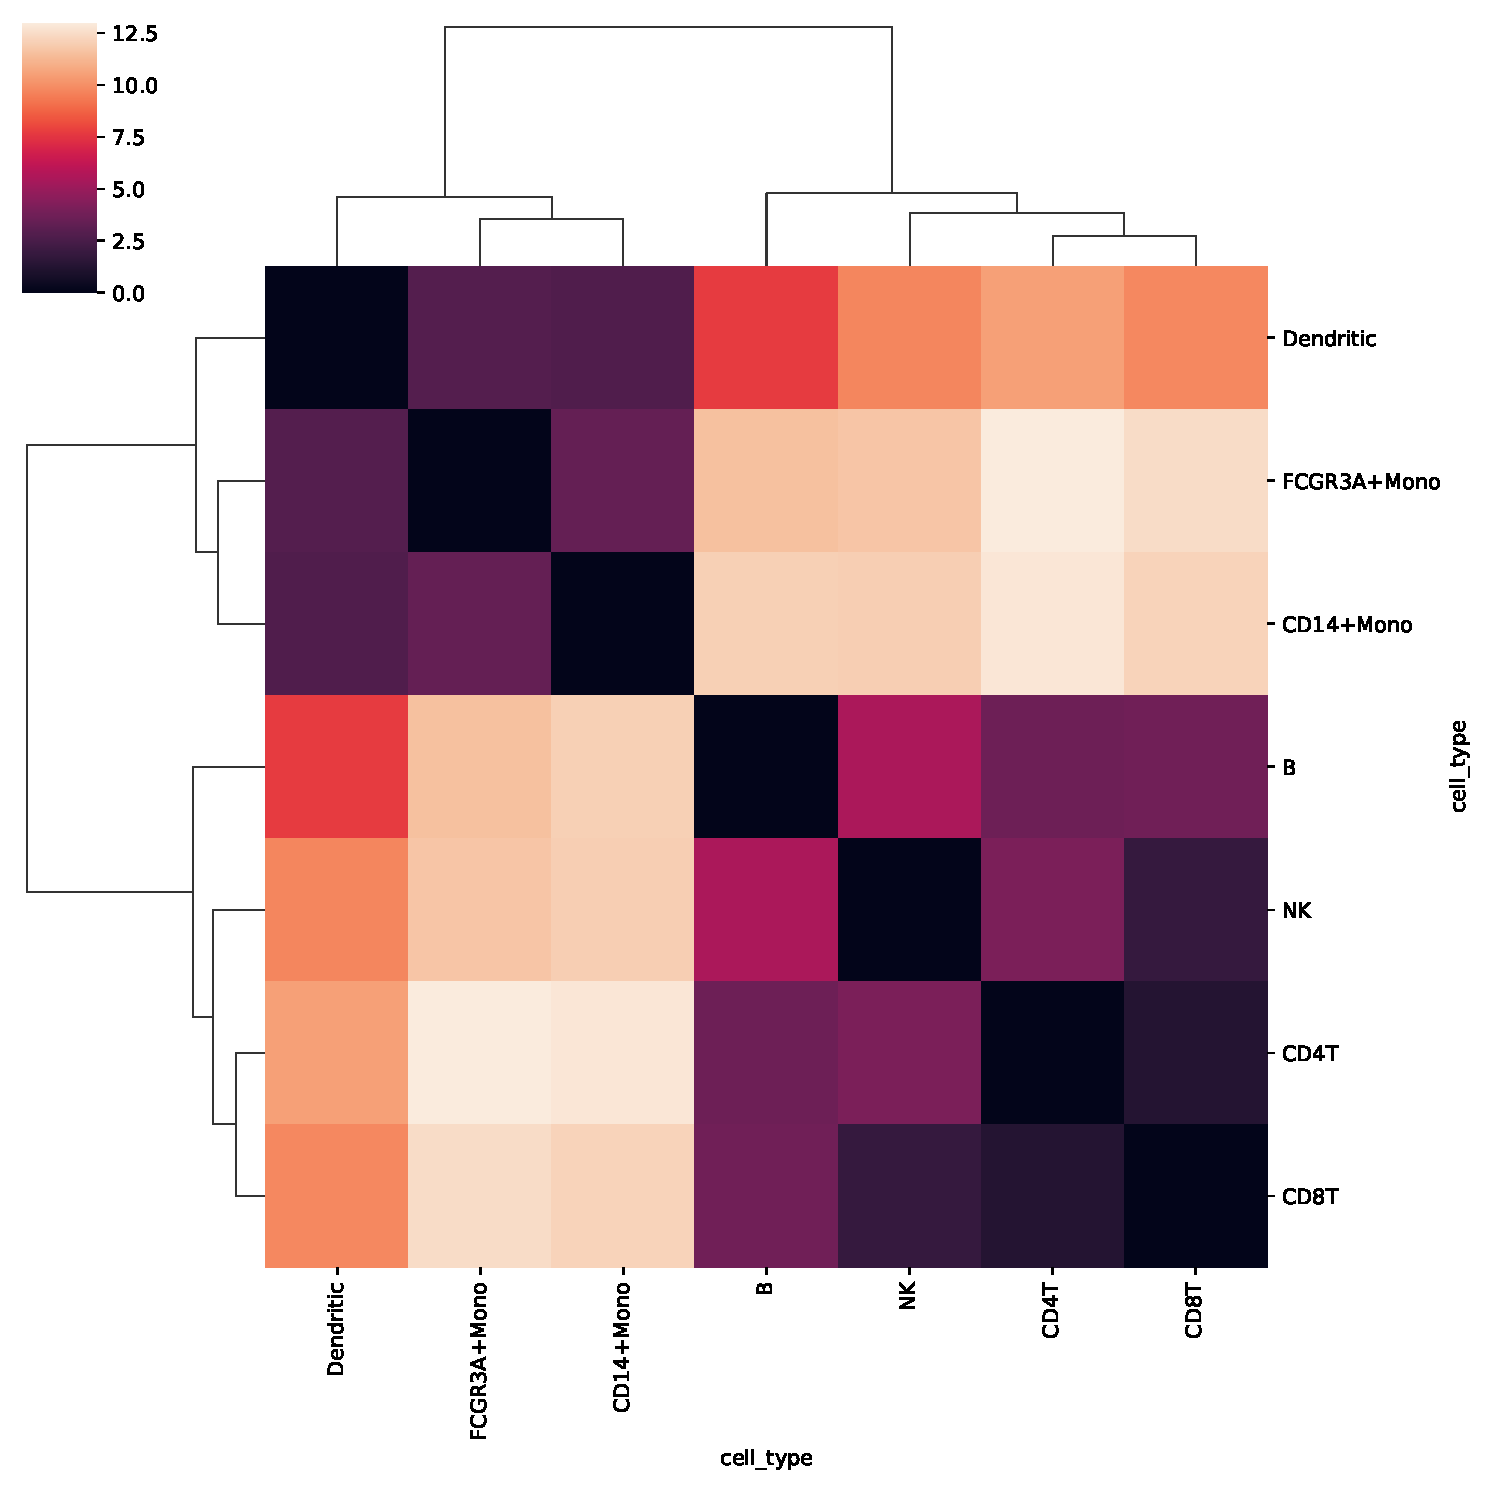
\includegraphics[width=\textwidth]{figures/pbmc_cell_type_edistance_clustermap.pdf}
        \caption{E-distance}
    \end{minipage} \hfill
    \begin{minipage}{0.4\textwidth}
        \centering
        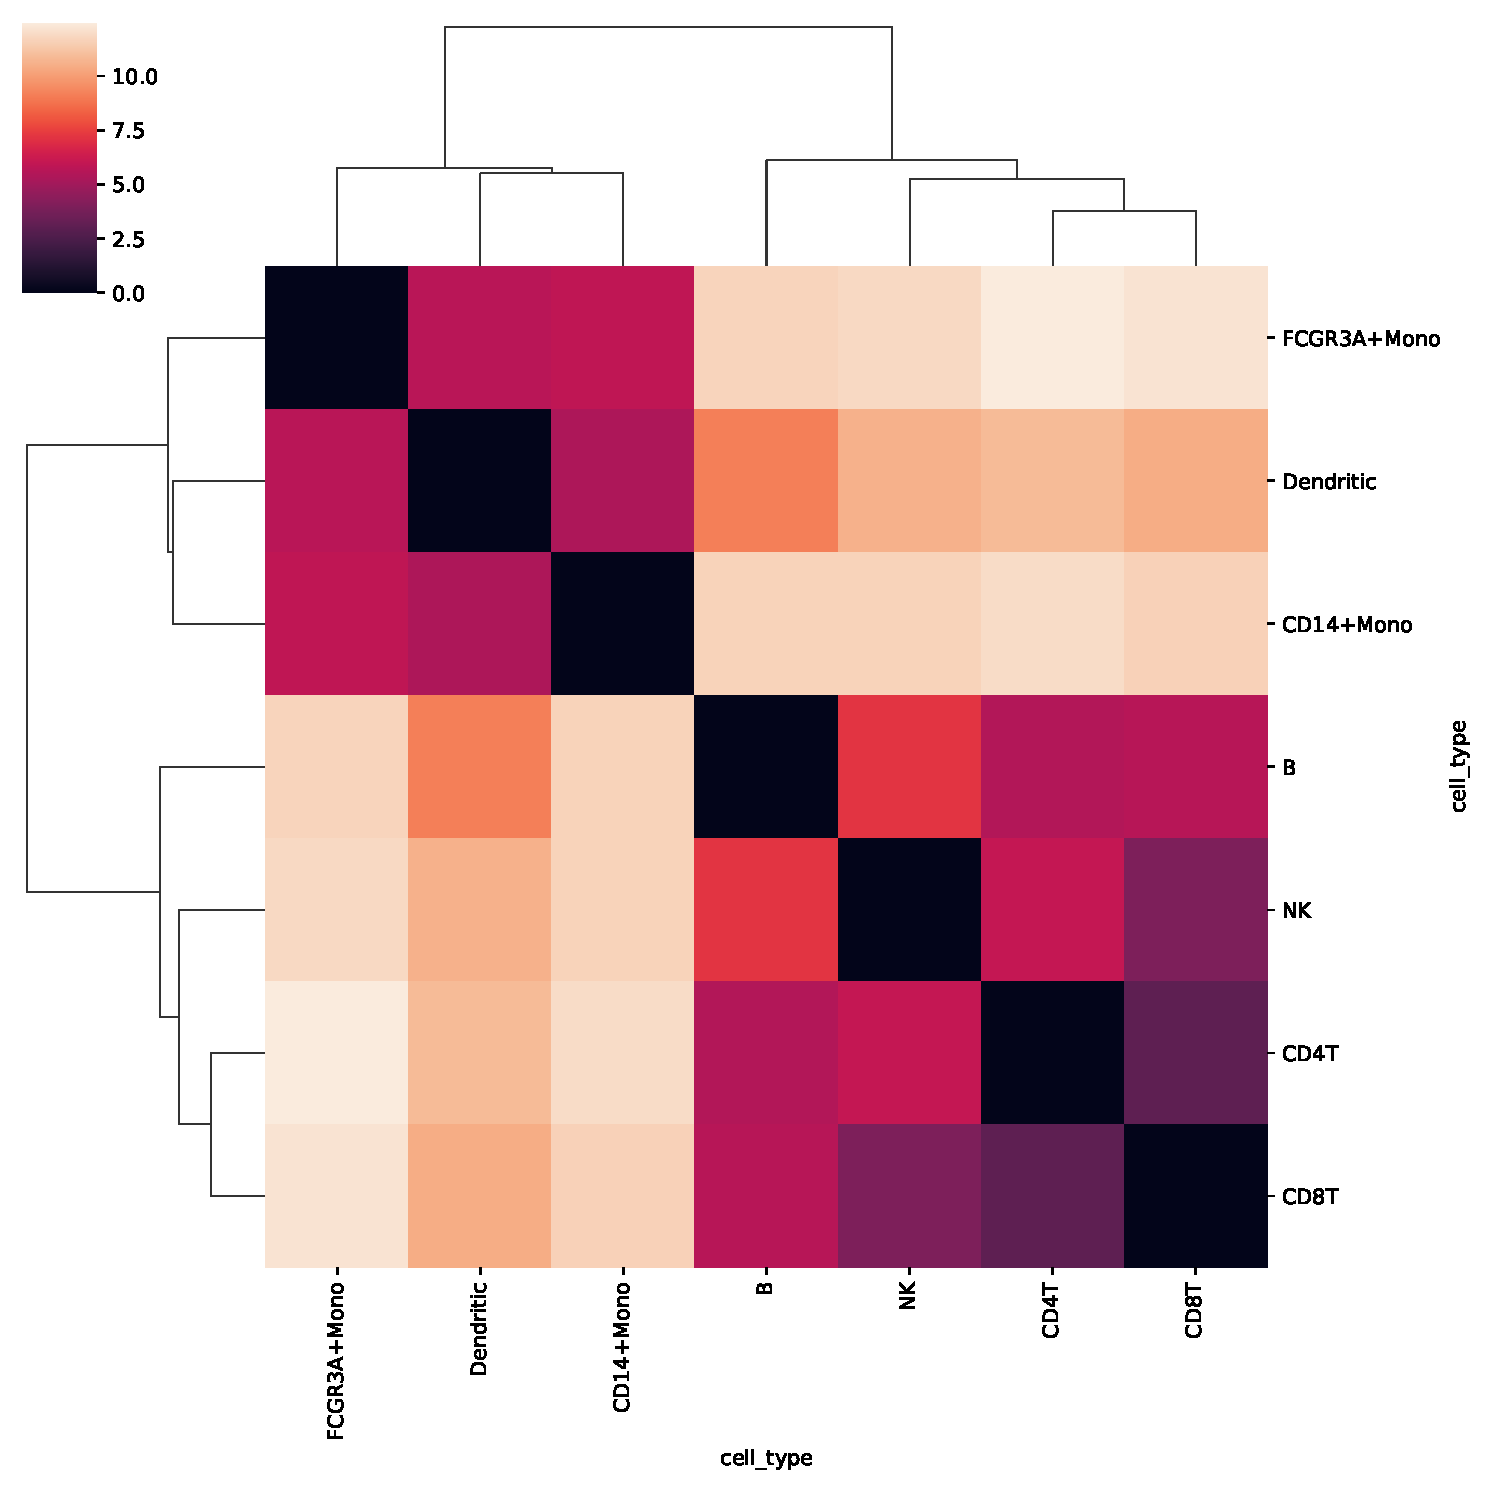
\includegraphics[width=\textwidth]{figures/pbmc_cell_type_euclidean_clustermap.pdf}
        \caption{Euclidean}
    \end{minipage}
    \vskip\baselineskip

    \begin{minipage}{0.4\textwidth}
        \centering
        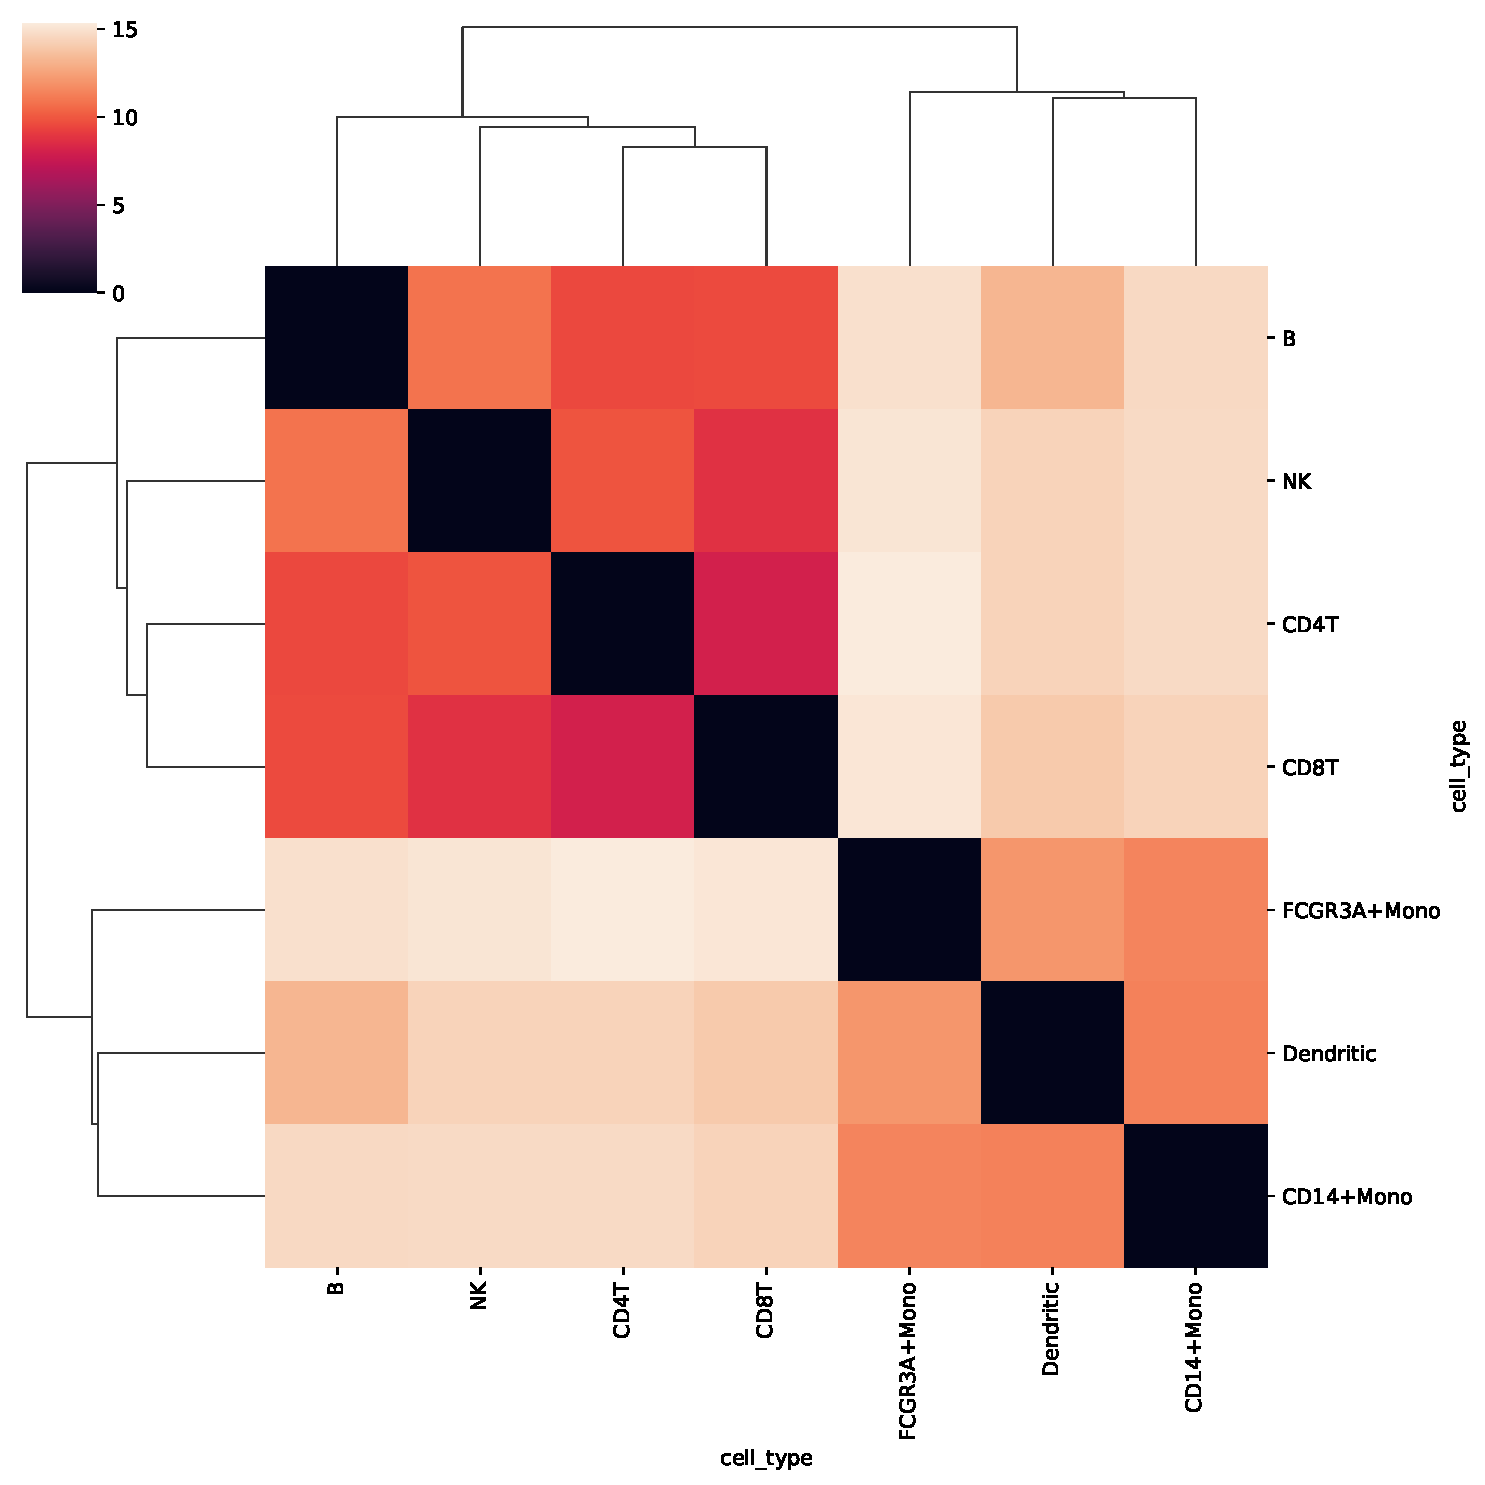
\includegraphics[width=\textwidth]{figures/pbmc_cell_type_mean_pairwise_clustermap.pdf}
        \caption{Mean pairwise}
    \end{minipage} \hfill
    \begin{minipage}{0.4\textwidth}
        \centering
        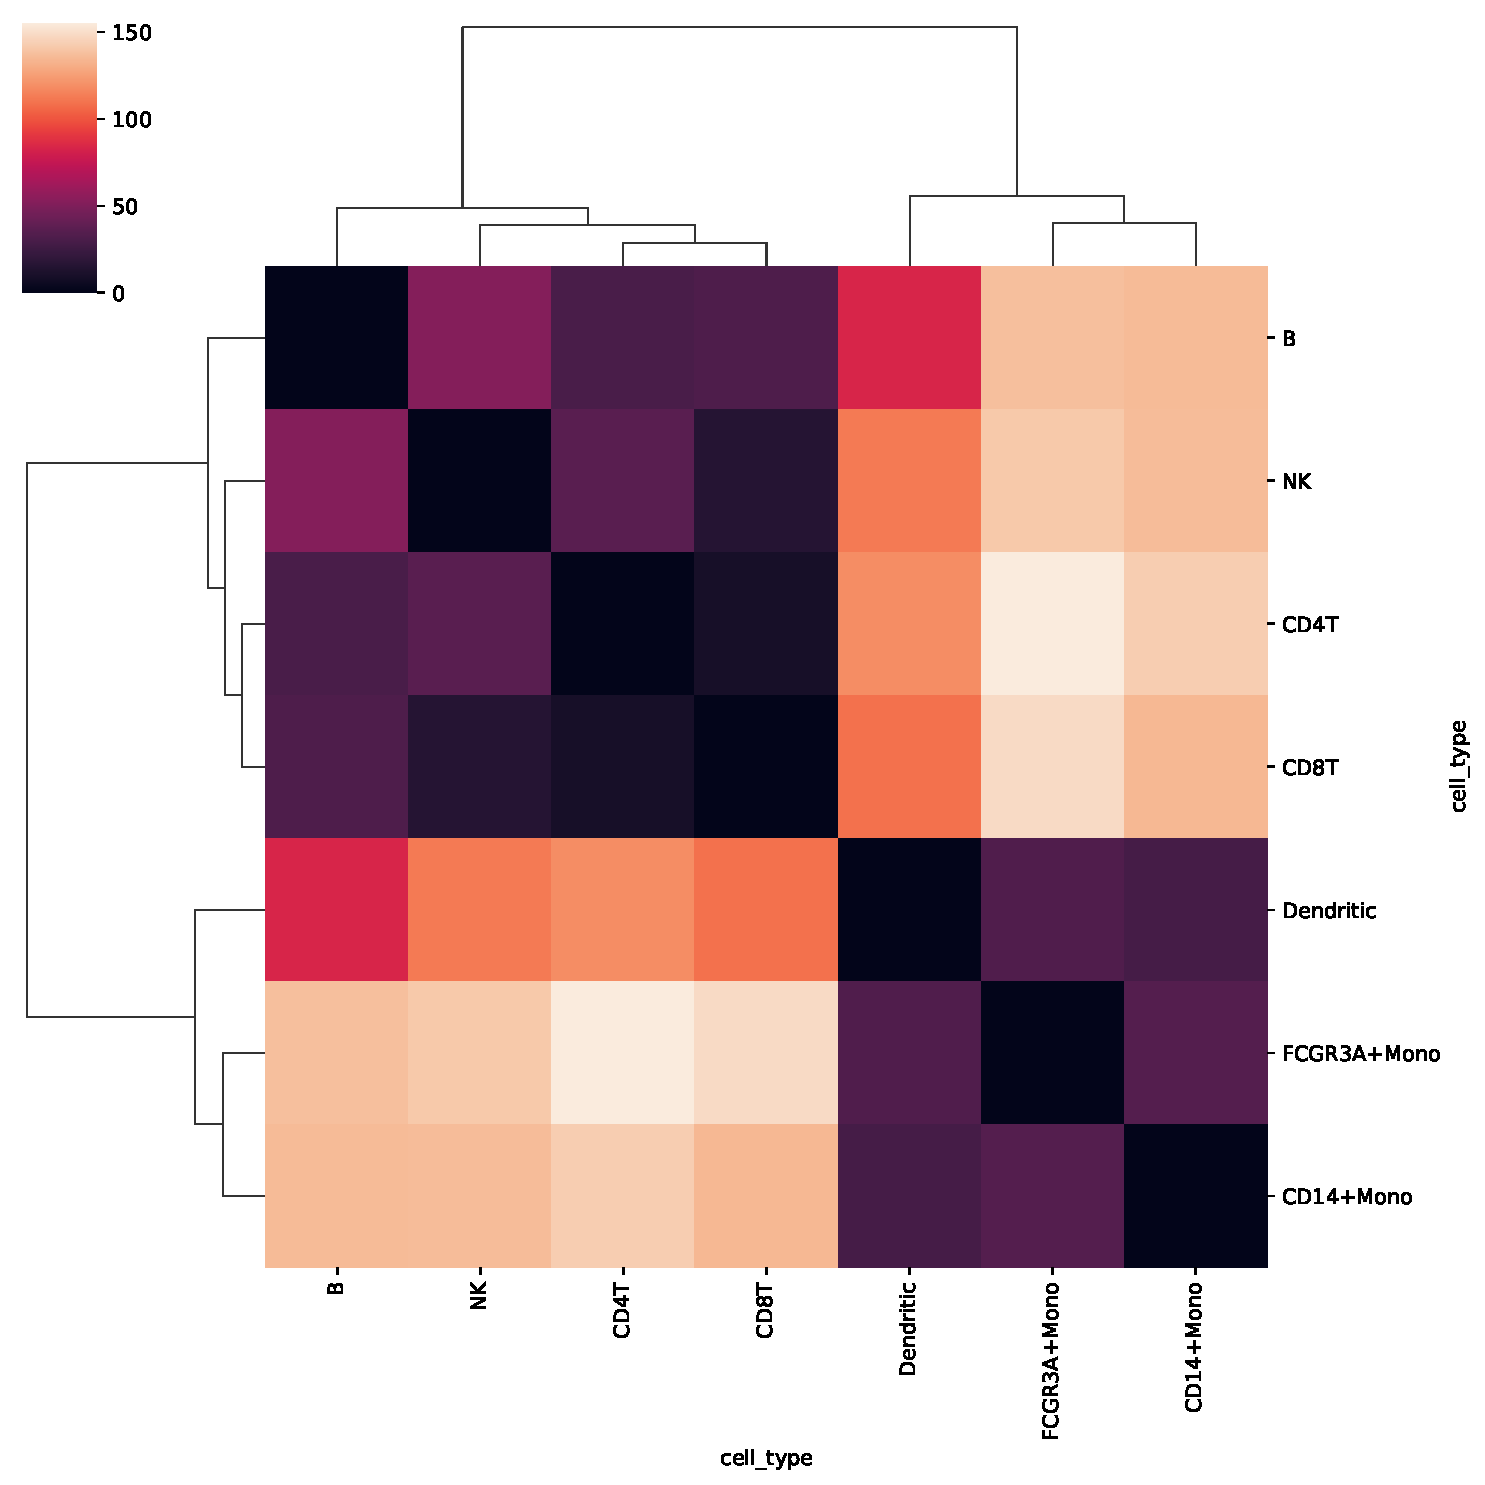
\includegraphics[width=\textwidth]{figures/pbmc_cell_type_mmd_clustermap.pdf}
        \caption{MMD}
    \end{minipage}
    \vskip\baselineskip

    \begin{minipage}{0.4\textwidth}
        \centering
        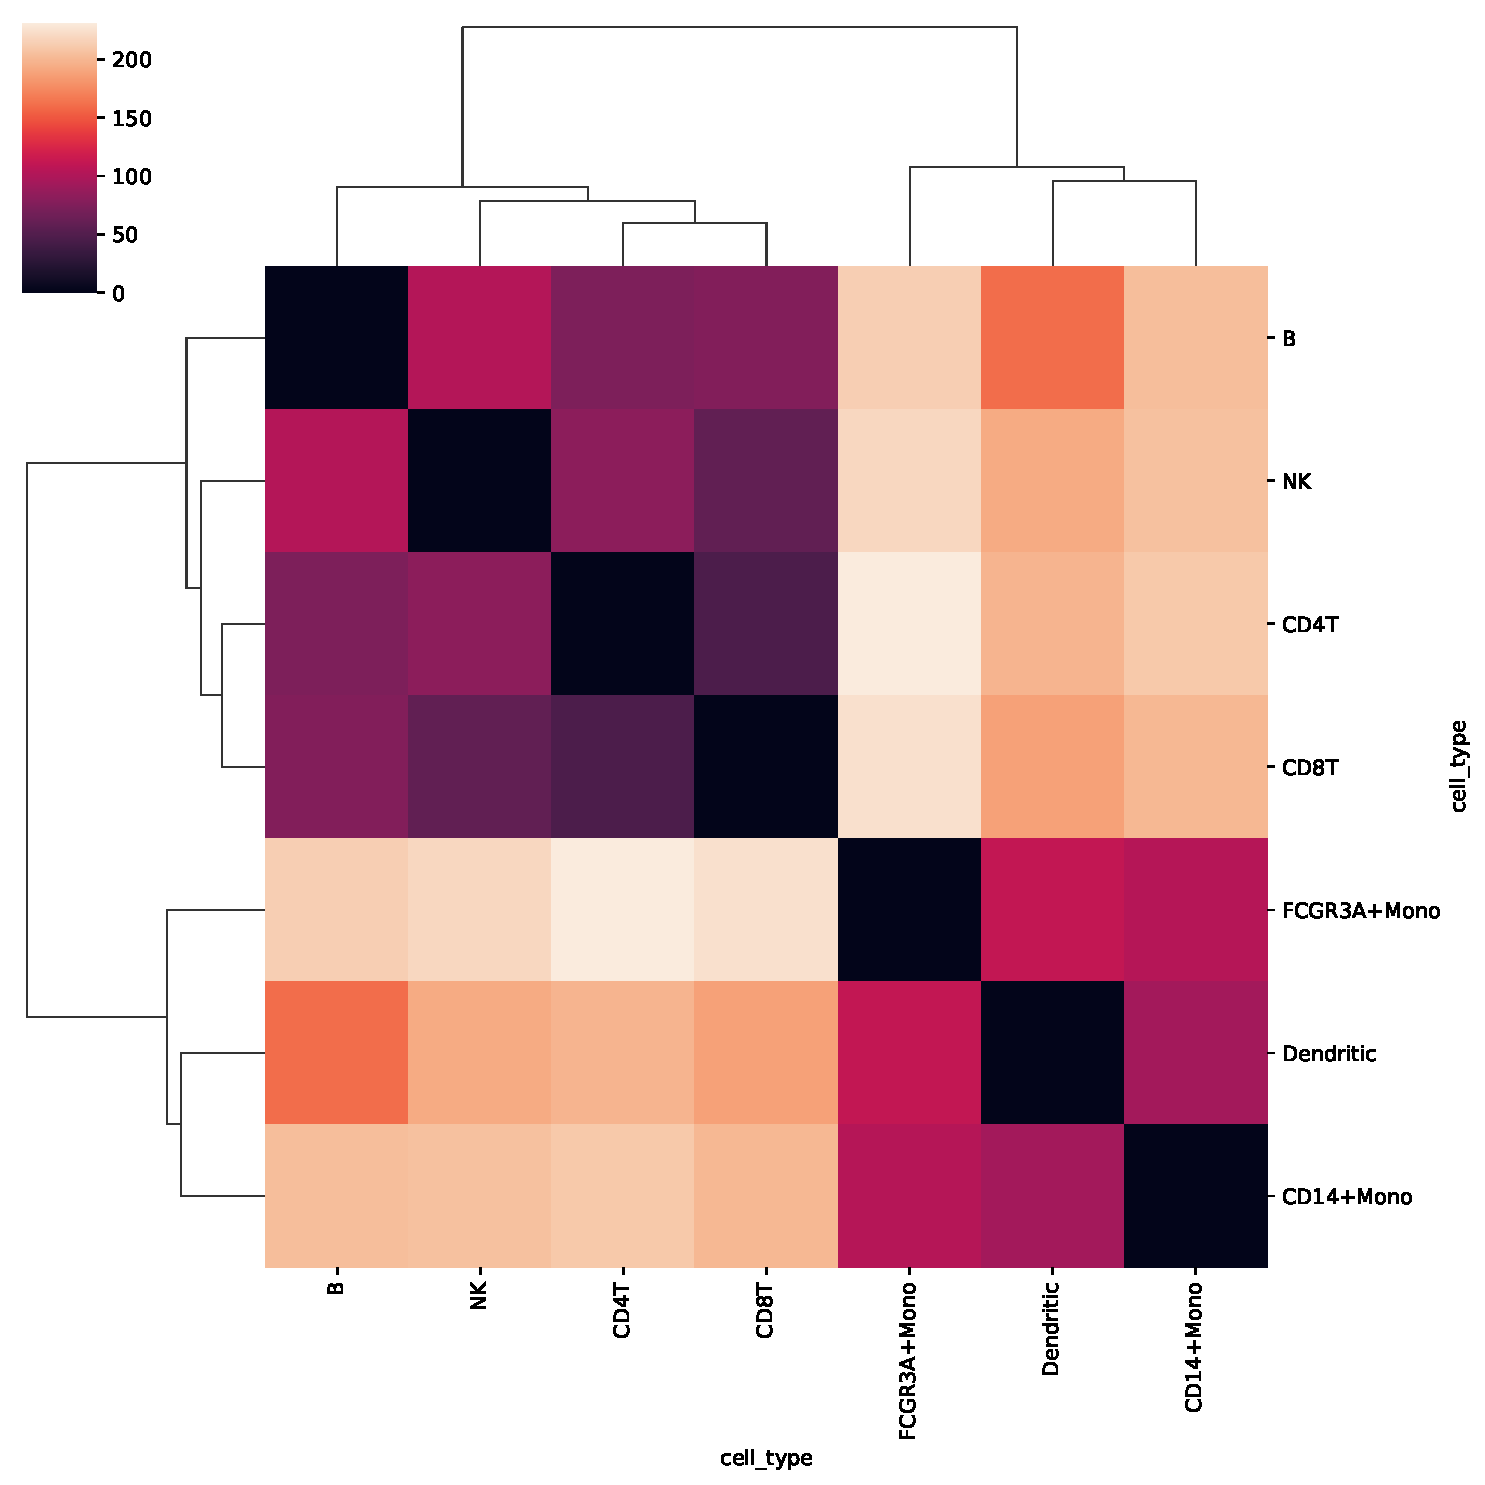
\includegraphics[width=\textwidth]{figures/pbmc_cell_type_wasserstein_clustermap.pdf}
        \caption{Wasserstein}
    \end{minipage}
    \caption{Distance metrics per cell type}
\end{figure}

\clearpage


\section{Experiment??}


